\documentclass[12pt,]{article}
\usepackage{lmodern}
\usepackage{amssymb,amsmath}
\usepackage{ifxetex,ifluatex}
\usepackage{fixltx2e} % provides \textsubscript
\ifnum 0\ifxetex 1\fi\ifluatex 1\fi=0 % if pdftex
  \usepackage[T1]{fontenc}
  \usepackage[utf8]{inputenc}
\else % if luatex or xelatex
  \ifxetex
    \usepackage{mathspec}
  \else
    \usepackage{fontspec}
  \fi
  \defaultfontfeatures{Ligatures=TeX,Scale=MatchLowercase}
\fi
% use upquote if available, for straight quotes in verbatim environments
\IfFileExists{upquote.sty}{\usepackage{upquote}}{}
% use microtype if available
\IfFileExists{microtype.sty}{%
\usepackage{microtype}
\UseMicrotypeSet[protrusion]{basicmath} % disable protrusion for tt fonts
}{}
\usepackage[margin=1in]{geometry}
\usepackage{hyperref}
\PassOptionsToPackage{usenames,dvipsnames}{color} % color is loaded by hyperref
\hypersetup{unicode=true,
            pdfkeywords={Recurrent Neural Networks, Machine Learning, Data Science, Probabilistic
Sequence Generation, Sentiment Analysis},
            colorlinks=true,
            linkcolor=red,
            citecolor=Blue,
            urlcolor=red,
            breaklinks=true}
\urlstyle{same}  % don't use monospace font for urls
\usepackage{graphicx,grffile}
\makeatletter
\def\maxwidth{\ifdim\Gin@nat@width>\linewidth\linewidth\else\Gin@nat@width\fi}
\def\maxheight{\ifdim\Gin@nat@height>\textheight\textheight\else\Gin@nat@height\fi}
\makeatother
% Scale images if necessary, so that they will not overflow the page
% margins by default, and it is still possible to overwrite the defaults
% using explicit options in \includegraphics[width, height, ...]{}
\setkeys{Gin}{width=\maxwidth,height=\maxheight,keepaspectratio}
\IfFileExists{parskip.sty}{%
\usepackage{parskip}
}{% else
\setlength{\parindent}{0pt}
\setlength{\parskip}{6pt plus 2pt minus 1pt}
}
\setlength{\emergencystretch}{3em}  % prevent overfull lines
\providecommand{\tightlist}{%
  \setlength{\itemsep}{0pt}\setlength{\parskip}{0pt}}
\setcounter{secnumdepth}{5}
% Redefines (sub)paragraphs to behave more like sections
\ifx\paragraph\undefined\else
\let\oldparagraph\paragraph
\renewcommand{\paragraph}[1]{\oldparagraph{#1}\mbox{}}
\fi
\ifx\subparagraph\undefined\else
\let\oldsubparagraph\subparagraph
\renewcommand{\subparagraph}[1]{\oldsubparagraph{#1}\mbox{}}
\fi

%%% Use protect on footnotes to avoid problems with footnotes in titles
\let\rmarkdownfootnote\footnote%
\def\footnote{\protect\rmarkdownfootnote}

%%% Change title format to be more compact
\usepackage{titling}

% Create subtitle command for use in maketitle
\newcommand{\subtitle}[1]{
  \posttitle{
    \begin{center}\large#1\end{center}
    }
}

\setlength{\droptitle}{-2em}

  \title{}
    \pretitle{\vspace{\droptitle}}
  \posttitle{}
    \author{}
    \preauthor{}\postauthor{}
    \date{}
    \predate{}\postdate{}
  
\usepackage{setspace}
% this is a lorem ipsum generator for adding dummy texts
\usepackage{lipsum}
\usepackage{tocloft}
% to make the first rows bold in tables
\usepackage{longtable}
\usepackage{tabu}
\usepackage{booktabs}
\usepackage{multirow}
% this makes list of figures appear in table of contents
\usepackage[nottoc]{tocbibind}
\usepackage{bbm}
\usepackage{morefloats}
\usepackage{float}
\floatplacement{figure}{H}

% referencing mutliple things with a single command - \cref
\usepackage{cleveref}


% this makes dots in table of contents
\renewcommand{\cftsecleader}{\cftdotfill{\cftdotsep}}
% to change the title of contents
\renewcommand{\contentsname}{Table of Contents}

% line numbers for review purposes
% this package might not be available in default latex installation 
% get it by 'sudo tlmgr install lineno'
%\usepackage{lineno}
%\linenumbers

% this allows checkmarks in the file
\usepackage{amssymb}
\DeclareUnicodeCharacter{2714}{\checkmark}

% to be able to include latex comments
\newenvironment{dummy}{}{}
\usepackage{booktabs}
\usepackage{longtable}
\usepackage{array}
\usepackage{multirow}
\usepackage{wrapfig}
\usepackage{float}
\usepackage{colortbl}
\usepackage{pdflscape}
\usepackage{tabu}
\usepackage{threeparttable}
\usepackage{threeparttablex}
\usepackage[normalem]{ulem}
\usepackage{makecell}
\usepackage{xcolor}

\begin{document}

\pagenumbering{gobble}

%\begin{titlepage}
\null\vspace{\fill}
\begin{center}
\Huge{\textbf{Composing Dynamic Soundscapes Using Neural Networks and Sentimental Input}}\\
\vspace*{\baselineskip}
\includegraphics[width=150px]{Images/untitled.png}\\
\vspace*{\baselineskip}
\Large{\textbf{CS350 Dissertation Project Final Report}}\\
University of Warwick, 2019\\
\vspace*{\baselineskip}
\Large{\textbf{Author}}\\
Harrison Wilde (u1600779)\\
Third Year, BSc Data Science\\
\vspace*{\baselineskip}
\Large{\textbf{Supervisor}}\\
Professor Graham Cormode\\
\vspace*{3\baselineskip}
\end{center}
% \end{titlepage}
\vspace{\fill}

\onehalfspacing

\hypersetup{linkcolor = black}
\newpage
\pagenumbering{roman}
\tableofcontents
\newpage
\setcounter{page}{3}
% list of figures have to be added manually to table of contents
\listoffigures 
\newpage
\setcounter{page}{5}

\listoftables
\newpage
\hypersetup{linkcolor = red}

\null\vspace{\fill}
\renewcommand{\abstractname}{Acknowledgements}
\begin{abstract}
\phantomsection  % required if using hyperref
\addcontentsline{toc}{section}{\abstractname}
\setlength\parindent{0pt}
\setlength{\parskip}{6pt plus 2pt minus 1pt}
\normalsize
\noindent
I owe great thanks to my personal tutor Professor Bärbel Finkenstädt, my trusted advisor Dr Matthew Leeke and my supervisor Professor Graham Cormode who have each shown consistent support on a personal, professional and academic level throughout my time at the University.

The support of my family and friends has been invaluable during this process; especially my mother Katie who has always been unwavering in her support of me in the pursuit of my aspirations.

I acknowledge and am grateful for the work of Mu Chen on his DeepSent project which forms the basis for some of the sentiment analysis carried out during this project. Additionally, the correspondence I shared with Nicolas Boulanger-Lewandowski and Daniel Johnson regarding their evaluation procedures was important in allowing me to compare the results of this project with their research (the work of these researchers is cited in the main body of the report).

Finally, I would like to thank all of the artists and musicians who gave feedback on my work or were featured in the training corpus; without their tireless work the world would be severely lacking in value and beauty. Most notably, the works of \href{https://www.youtube.com/watch?v=JKsVsEXZXe8}{Ryuichi Sakamoto}, \href{https://music-from-memory.bandcamp.com/track/call-me-2}{Gigi Masin}, \href{https://youtu.be/vveVs8axQRc}{Jónsi and Alex Somers}, \href{https://helloflora.bandcamp.com/track/cecilia-lake}{Jamison Isaak} and \href{https://bvdub.bandcamp.com/track/ember-1}{Brock Van Wey} have shaped my years as an undergraduate and offered a great deal of creative and intellectual stimulation as well as instilling a great appreciation for the world and its people.
\end{abstract}
\vspace*{\baselineskip}
\vspace{\fill}
\newpage



% - convey the essence of your project
% - be self-contained
% - state significant results/outcomes/achievements
% 1. Purpose
% 2. Methodology/Project Design
% 3. Findings/Contribution
% 4. Research Limitations/Future work
% 5. Practical Implications/Conclusions


\null\vspace{\fill}
\renewcommand{\abstractname}{Abstract}
\begin{abstract}
\phantomsection  % required if using hyperref
\addcontentsline{toc}{section}{\abstractname}
\setlength\parindent{0pt}
\setlength{\parskip}{6pt plus 2pt minus 1pt}
\normalsize
\noindent
This dissertation investigates deep sequential learning techniques in context of the very complex, human and artistic challenge of musical composition: an application of artificial neural networks that encourages innovation through the implementation of cutting-edge research.

Model architectures are devised that exhibit progression in their ability to learn rich temporal and relative harmonic structures, as well as in generating music which is dynamic and conscious of a user-supplied mood or sentiment. To achieve this, models are trained with a generalised representation of digital musical scores incorporating data on analysed sentiment and dynamics.

The models are versatile and performant, such that they compete with and in some cases surpass the current state-of-the-art quantitatively, qualitatively and computationally. New functionality is also implemented such as the incorporation of sentimental input and independence from certain musical characteristics of the training data, e.g. key and genre. This is achieved through the unification of techniques spanning the field of deep learning in order to minimise model complexity whilst maximising effectiveness.

Further work would likely leverage higher-quality datasets as they become available alongside any new developments surrounding artificial neural networks to aid in capturing the long-term dependencies present in musical data.
\end{abstract}
\vspace{\fill}
\vspace*{\baselineskip}
\hrule
\vspace{3px}
\begin{footnotesize}
\textbf{Keywords:} Recurrent Neural Networks, Musical Composition, Machine Learning, Probabilistic Sequence Generation, Sentiment Analysis
\end{footnotesize}
\newpage

\pagenumbering{arabic}

\hypertarget{introduction}{%
\section{Introduction}\label{introduction}}

The project undertaken and discussed in this report was concerned with
exploring the problem space of musical composition from a probabilistic
and algorithmic perspective, with added extensions regarding the
incorporation of a user's mood and some performative characteristics of
composition. Numerous approaches exist to offer a basis upon which new
ideas and techniques could be applied. These approaches include
Markovian techniques, symbolic generative models, evolutionary
algorithms, neural networks and beyond. Some of the more historical work
has already been surveyed
{[}\protect\hyperlink{ref-nierhaus2009algorithmic}{1}{]}; this report
focusses primarily on new developments in the field of deep neural
networks and their application and effectiveness regarding musical
composition. Justification for this focus is provided throughout the
course of the report.

Deep neural network architectures have led to significant improvements
in many similar contexts and have already replaced some traditional
methods entirely (mainly in the areas of translation, speech recognition
and image-video analysis). The importance of this paradigm shift is
clear; this project explores the application of some techniques from
these other fields to musical composition alongside the deep learning
approaches that have already been covered by considering and applying
both musical and mathematical theory.

\hypertarget{motivation}{%
\subsection{Motivation}\label{motivation}}

Since recurrent neural networks rose to prominence in the 1990s, deep
learning has shown great promise in the task of completely automated
algorithmic musical composition. This is a complex application exploring
some challenging computational and philosophical questions in terms of
how the ``rules'' of music might be correctly encapsulated in order to
compose musical pieces to eventually compete with what has always been
an almost exclusively human process. There is still no real solution to
this problem despite advances in other creative applications of deep
learning meaning there are still a multitude of possibilities to explore
and assess.

There would be contention in explicitly defining rules for something as
complex and subjective as music; this is where deep learning's relative
impartiality and awareness is desirable to aid in potentially
understanding abstract concepts behind the process of musical
composition. Indeed, it has already proven effective on a number of
previously inaccessible tasks where patterns were not thought to be
present, or at least were difficult to capture due to the perception
that some tasks are limited by requirements for human intuition and
judgement.

Music is an intrinsically complicated form of data; it is difficult for
machines to understand due to the presence of long-term dependencies and
complex structures throughout. These structures take on multiple forms
but can be roughly categorised into temporal, harmonic and performative
structures: a piano player must play in time, in key and also in a way
which sounds pleasant through the use of tension, control in their
playing style and personal additions of flair.

It is these challenges that form the basis of the motivation for this
project. Other researchers have been contributing to this area for
decades and this project hopes to further this path of exploration.
Moreover, there are great potential implications beyond just musical
composition, as recurrent neural networks and deep network architectures
are beginning to be applied to a myriad of critical tasks in business,
science and society
{[}\protect\hyperlink{ref-deng2014deep}{2}{]}--{[}\protect\hyperlink{ref-goodfellow2016deep}{4}{]}.

Many use cases for the outputs of this project specifically also come to
mind, whether it be integration with current digital solutions for the
composition of music, or the creation of entirely new services such as
procedurally generated soundscapes to match the immersion offered by VR
media, or even personal digital assistants which could utilise the work
exhibited here to compose or recommend music based on a user's mood.

The complexity of the task and the intrigue its outputs generate from a
creative and technical perspective provide a great deal of motivation.
It is likely that the innovation required to make progress in musical
composition may be applicable to some of the aforementioned tasks where
deep learning is already beginning to show promise. Great computational
challenges like these could be compared to similarly ambitious problems
in engineering and classical science such as space travel, which have
offered countless by-products integral to modern society.

\hypertarget{a-brief-history-of-computational-approaches-to-composition}{%
\subsection{A Brief History of Computational Approaches to
Composition}\label{a-brief-history-of-computational-approaches-to-composition}}

The number of research papers regarding musical composition has
increased significantly in recent years alongside the increase in
popularity of deep learning techniques. However, the task and potential
solutions pre-date deep learning entirely:

\begin{itemize}
\tightlist
\item
  Markov chains were first formalised in the 1900s and were used to
  string together segments of score or individual musical notes based on
  a set of transition probabilities in order to probabilistically
  generate sequences of music following initial conditioning. Iannis
  Xenakis was one of the first to consider this and contributed a lot of
  discourse regarding Markovian approaches in the early years of the
  problem {[}\protect\hyperlink{ref-luque2009stochastic}{5}{]}.
\item
  Hidden Markov models and recurrent neural networks were applied in an
  attempt to overcome the main limitations of Markov chains regarding
  their inflexibility and lack of represented understanding beyond the
  reproduction of sub-sequences of the original pieces that were used to
  condition them. These techniques first rose to prominence in the
  1980s. The early attempts were limited by a break-down in coherence
  beyond a small neighbourhood of notes; the outputs would often lack
  any real structure and explode into chaos or vanish into silence.
  However, these approaches did start to incorporate the possibility of
  understanding polyphonic (multiple notes being played at a time,
  incorporation of chords and polyrhythms etc.) input and generating
  polyphonic output due to their ability to deal with more complex
  representations and structures.
\item
  In the early 2000s, some improvements on RNNs which aimed to solve
  some of the aforementioned issues were first applied to composition.
  The first published attempt was made by Doug Eck in 2002
  {[}\protect\hyperlink{ref-eck2002finding}{6}{]} and utilised Long
  Short-Term Memory Units
  {[}\protect\hyperlink{ref-gers1999learning}{7}{]} as a potential
  solution to the flaws associated with RNNs.
\item
  Doug now leads the Magenta team at Google Brain
  {[}\protect\hyperlink{ref-magenta}{8}{]} who have created a myriad of
  models focussing mainly on assisted accompaniment for musicians or
  improvisation with a user. They have continued to apply LSTMs to these
  problems as well as variations on the Transformer (a sequence model
  based on self-attention) pioneered by Huang et al.~in 2018
  {[}\protect\hyperlink{ref-huang2018improved}{9}{]}.
\item
  The field has fragmented in recent years as teams such as Magenta
  focus more heavily on interactions with a user, whilst others have
  started focussing on raw audio rather than MIDI (a universal and
  compact digital scoring format and standard for composition) and
  character representations which are considered to be the standard
  training data formats. The raw audio approach has huge requirements in
  terms of data and training time meaning that it is still currently
  somewhat inaccessible. Despite this, some notable and relatively
  successful research has been carried out by Google's Deepmind on the
  WaveNet project {[}\protect\hyperlink{ref-oord2016wavenet}{10}{]}.
  Other, less creatively focused applications have started to become
  popular as well, especially within the field of speech synthesis.
\item
  There is currently no documented work on sentiment-influenced
  automatic musical composition, motivating this project to include it
  as part of its objectives. There is however a relatively robust body
  of work surrounding sentiment analysis of images and more
  theoretically of humans.
\end{itemize}

There is further discussion to this history if the reader is inclined
{[}\protect\hyperlink{ref-mediumkylemcdonald}{11}{]},
{[}\protect\hyperlink{ref-libdlmusic}{12}{]}; the list above covers the
most relevant milestones with the aim of providing some historical
context to the starting point of this project.

\hypertarget{research-objectives-and-project-requirements}{%
\subsection{Research Objectives and Project
Requirements}\label{research-objectives-and-project-requirements}}

The project was initialised with two main components and associated
objectives, these components were:

\begin{itemize}
\tightlist
\item
  The development of a \textbf{means of transcription} in order to
  create training data for a model. Accompanied by the decision of
  \textbf{a medium around which to build and train the proposed models},
  i.e.~the training data \emph{format}. The main choice was between raw
  audio and MIDI data. Other options do exist such as ABC notation (also
  known as scoring notation, letters representing notes and numbers
  representing octaves in sequence), but these were quickly discounted
  due to limitations surrounding the acquisition of training data and
  also the lack of practical applications for the output when compared
  to raw audio and MIDI which more richly capture the temporal and
  dynamic structures present in music.
\item
  The design and implementation of a model architecture providing
  \textbf{a means of composing polyphonic musical pieces based on
  training data and sentimental input from a user}; this question is
  heavily influenced by the answer to the one posed above in that the
  structure of the training data informs potential architecture choices.
  Consideration was to be made of all the aforementioned historical
  approaches, before going on to consider the possibilities of recent
  innovations in the deep learning field. This component was to be the
  main focus for technical innovation during this project.
\end{itemize}

Generative probabilistic models such as hidden Markov models and
recurrent neural networks were the main subject of exploration
throughout the research section of this project. The main goals may be
summarised by the desire to build a versatile model whose outputs are at
best indistinguishable from that of a human and at worst impressive in
terms of their structural and harmonic coherence. A novel approach was
to be built and assessed to determine its place amongst the current
cutting-edge systems through comparative qualitative and quantitative
evaluation. Contributions from this report will hopefully form the basis
of future research and enable continued development within this problem
space. To achieve this, it was first necessary to gain a complete
understanding of the current research landscape and formulate comparable
and relevant metrics with which to evaluate the project in context of
this existing work.

The designed and implemented models draw inspiration from many fields
that reveal deep learning as an increasingly effective solution provided
high-quality data is present. This inspired investigation into different
means of creating and representing training data for the task as well as
consideration of the current ``standards'' with regards to datasets used
by other researchers.

The requirements placed on the model architecture are as follows:

\begin{itemize}
\tightlist
\item
  MIDI digital score sourced from existing datasets and transcribed
  audio should be utilised to condition a neural network's parameters
  such that it can understand and replicate the structure and dynamics
  of its inputs in generated compositions. Transcribing raw audio into a
  novel training corpus is desirable in order to allow a user to train a
  model to compose within their own musical tastes.
\item
  The system should adopt an intermediate, tractable representation of
  the MIDI data; this representation should encompass:

  \begin{itemize}
  \tightlist
  \item
    The temporal structure of its training pieces accounting for pauses,
    changes in tempo and other dynamic intricacies of the input.
  \item
    The harmonic structures present in the training data including the
    chords, progressions and key of its pieces, by effectively capturing
    the different notes and combinations of notes present.
  \item
    The performative structures, i.e.~dynamics of a piece through the
    way in which it is played. This could include information regarding
    the length and strength with which different notes are played, so
    that the model might also learn to play with a more human-sounding
    style.
  \end{itemize}
\item
  Generation should be done using a model post-training and should allow
  for additional parameters to be supplied by a user such as a starting
  `inspirational' state and the length the composed piece should be.
\item
  Generated compositions should be influenced by a user's inputted mood
  or sentiment; meaning the training data must also incorporate a
  representation of this sentiment.
\item
  The model should be independent of any particular genre or
  pre-training, such that it can be applied to a wide variety of genres
  and contexts.
\item
  The system should effectively solve or improve upon some of the issues
  present in current solutions and ideally progress beyond previous work
  in terms of accessibility and computational requirements by
  prioritising efficiency and parsimony (minimising complexity and total
  parameters without sacrificing effectiveness) in a model which is
  built with an awareness and respect for musical theory without being
  tied to it.
\item
  Evaluation should be carried out quantitatively and qualitatively to
  address the main goals mentioned above, namely whether the model is
  capable of effectively imitating human composition in the opinion of
  human listeners but also using some quantitative metric that is
  comparable to previous work.
\end{itemize}

Additionally, in order to facilitate the above main requirements, a
means of audio to MIDI transcription must be proposed and implemented
that is effective and accessible such that others might replicate this
work or potentially package it into a user-friendly solution for anyone
to interact with and make use of the technical innovations described
here. This transcription system should produce outputs of the highest
possible accuracy so that it can be used to generate training data of
the highest possible quality (involving minimal noise and incorrect
notes which would potentially damage a model's capacity to learn
effectively).

Some stretch goals were highlighted early in the project's specification
but were ultimately not included due to their lack of contribution to
the aforementioned goals and in the interest of wanting to focus on
building the best model architecture and representation possible. The
main stretch goals were:

\begin{itemize}
\tightlist
\item
  A website hosting a pre-trained model to allow for interactivity for
  non-expert users and to potentially facilitate a larger scale
  qualitative assessment of the project using feedback from interactions
  with this web application.
\item
  Utilising existing solutions in image analysis (an area which is
  considerably more developed than this one) to analyse the sentiment of
  an image and then feed this sentiment in as input rather than having
  the user input it manually.
\end{itemize}

These objectives required significant background and technical knowledge
to be gathered as well as a rigorous development process, both of these
are discussed in the \protect\hyperlink{methodology}{Methodology
section}. The decisions made throughout were often reliant on context
provided by the historical timeline of the problem and the accrued
collection of related work relevant to this problem space.

\hypertarget{related-work}{%
\section{Related Work}\label{related-work}}

The methods and solutions described here tend to be linked but are
discussed with respect to the two main components mentioned previously.

\hypertarget{musical-data-transcription-and-representation}{%
\subsection{Musical Data, Transcription and
Representation}\label{musical-data-transcription-and-representation}}

\hypertarget{justification-for-using-midi-over-raw-audio}{%
\subsubsection{Justification for Using MIDI Over Raw
Audio}\label{justification-for-using-midi-over-raw-audio}}

The main goal regarding transcription and representation was to build a
large library of data with enough engineered features for the model to
successfully produce meaningful output. As was already alluded to, it
becomes clear following initial investigation that the use of raw audio
data involves a much larger computational overhead making it an
infeasible approach given the time-scale and resource allocation of this
project (as well as the fact that often projects in this space feature
multiple postgraduate authors). MIDI as a format is a standard in the
world of digital musical equipment and production as well as in research
surrounding this problem (the majority of the papers cited here utilise
MIDI to some extent); its equivalence with musical score and provision
of deterministic data on what notes are played, when they are played and
how they are played lends itself perfectly as a format to the task of
training a model to compose music.

These characteristics are clear and separable such that there is no
confounding information regarding the music contained; a model can learn
the ``rules'' of music through considering the same things a human would
consider when composing a piece. Whereas raw audio includes many
artefacts and intricacies which obscure these features as well as being
potentially too complex for much of the current landscape of machine
learning, especially when compared to MIDI and similar representations
{[}\protect\hyperlink{ref-dai2018music}{13}{]}.

Raw audio contains data regarding the timbres of different instruments,
performance characteristics etc. which are incredibly difficult for
current technologies to comprehend; MIDI provides an excellent middle
ground especially with the inclusion of velocity data which still
captures some of the human performative elements of a piece in a
quantitatively justifiable way. Structurally, it is much easier to
represent music using this compositional data which is abstracted away
from factors such as the instrument it is played on and a player's
personal style.

The only documented attempt of working with raw audio that showed any
potential for success was carried out by Google
{[}\protect\hyperlink{ref-oord2016wavenet}{10}{]} who are significantly
advantaged in terms of their resources.

\hypertarget{midi-transcription-techniques}{%
\subsubsection{MIDI Transcription
Techniques}\label{midi-transcription-techniques}}

Google's work can still be leveraged however: their Magenta team created
a TensorFlow sub-package focussing on musical composition, transcription
and other artistic endeavours. This work includes an ``Onset Frames''
model for MIDI transcription
{[}\protect\hyperlink{ref-hawthorne2017onsets}{14}{]} that is
pre-trained on classical piano music and has performance beyond all
other options in terms of the calculated F1-score and accuracy when
comparing the differences between the model's generated transcriptions
and their ground truths (i.e.~considering true / false positive /
negative notes transcribed by the systems). The data for these
comparisons is present in the paper as an ablation study carried out to
justify the innovative features incorporated into the architecture it
presents.

The architecture mainly relies on convolutional kernels to capture
features in the raw audio and map them to MIDI notes. Due to this, it
requires a great deal of training data to be effective and tends to
perform best in transcribing the genre it was trained on, though it is
still reasonably effective for other styles of musical input. Many other
attempts have applied convolutional neural networks to the task of
musical transcription
{[}\protect\hyperlink{ref-bereketai}{15}{]}--{[}\protect\hyperlink{ref-sarnatskyi2017music}{17}{]}
with promising results at their resolutions indicating that this
application of CNNs is at the forefront of the musical transcription
task.

It is worth noting that this process exemplifies one of the largest
challenges and complexities in this project: using machine learning to
\emph{generate} the data used to then train a model to compose music in
a similar way introduces a lot of uncertainty and dependence between
these two components. Any issues with this first component would
propagate throughout the entire project, meaning that it was important
to assess the model's quantitative performance using comparable
methodology and pre-existing datasets, on top of fulfilling the goals of
the project qualitatively by building an end-to-end system incorporating
the creation of training data from raw audio as described.

Other approaches to transcription pre-date the use of CNNs and focus on
more traditional signal processing techniques. Of these, WaoN
{[}\protect\hyperlink{ref-waon}{18}{]} appeared to be the most accurate
and well-documented. Cross-validation and assessment between the ``Onset
Frames'' model and WaoN was carried out; often one was better than the
other depending on the structure and content of the raw audio source.

\hypertarget{pre-existing-datasets}{%
\subsubsection{Pre-Existing Datasets}\label{pre-existing-datasets}}

Some pre-existing datasets were also investigated and utilised in
training and evaluating the models to provide an alternative to the
training data generated using the techniques discussed above and
hopefully mitigate some of the concerns and uncertainties raised in
using non-perfect data to train a model. Of these, the most notable are
the MAESTRO dataset {[}\protect\hyperlink{ref-maestro2018}{19}{]} which
includes over 1200 pieces in MIDI and \texttt{.wav} format spanning 170
hours, alongside four datasets considered to be the current standard in
evaluating models based on their usage in other musical composition
research papers. These are:

\begin{itemize}
\tightlist
\item
  JSB Chorales, a corpus comprised of 382 four-part chorales by Bach and
  recorded to MIDI by John Sankey on a digital piano.
\item
  MuseData, a library of 784 orchestral and classical pieces spanning
  numerous composers recorded as MIDI data, compiled through sponsorship
  from the CCARH at Stanford University
  {[}\protect\hyperlink{ref-ccarh}{20}{]}.
\item
  Nottingham, a corpus of 1038 folk tunes transcribed to MIDI.
\item
  Piano-Midi.de, a collection of 125 classical piano piece MIDI
  transcriptions.
\end{itemize}

All of these datasets are hosted online with their original
test:train:validation splits included; hosting is provided by the
University of Montreal where Boulanger-Lewandowski et al.~carried out
research and evaluation in automated musical composition
{[}\protect\hyperlink{ref-boulanger2012modeling}{21}{]}. Their
evaluation procedure has since been replicated in numerous works,
inviting its inclusion in this project as a means of measuring the
progress made in relation to previous attempts. Additionally, the
availability and utilisation of these datasets was integral to beginning
development on the model architectures in a timely manner without having
to rely on a completely realised MIDI transcription solution.

\hypertarget{possible-representations}{%
\subsubsection{Possible
Representations}\label{possible-representations}}

Almost all of the cited papers involve a variety of unique approaches to
representing MIDI or audio data numerically in a format that captures
the relevant features to facilitate acceptable training of a model. Most
utilised some form of one-hot binary mapping to the keys on a piano or
used symbolic text processing approaches which generated strings of
notes based on the classical lettered notation of music (A1, B2, C4 etc.
with the number indicating which octave on the piano each note belongs
to).

\hypertarget{competitive-existing-solutions}{%
\subsection{Competitive Existing
Solutions}\label{competitive-existing-solutions}}

\hypertarget{neural-network-approaches}{%
\subsubsection{Neural Network
Approaches}\label{neural-network-approaches}}

Neural Networks are undoubtedly a very active area of research; a lot of
which is relevant or could even be directly applied to this project.
Popular scientific discourse
{[}\protect\hyperlink{ref-alextavgen}{22}{]} showcases some of the
capabilities of recurrent neural networks working on generating code,
text and images. Music is considered to be a more challenging feat for
these systems, which is perhaps intuitive given its continuous and often
complex nature.

Google's Magenta project has already been mentioned as one of the main
proponents of research in this area. Magenta's collection of pre-trained
models is testament to the promise of this platform; more specifically
there are pre-trained models available which produce improvisation,
polyphony and interpolation of input pieces
{[}\protect\hyperlink{ref-magentamodels}{24}{]}. The aim of this project
is to build and train a model sitting somewhere between these existing
ones, one which is capable of generating inspired sequences of chords
and notes and then recurrently feeding these generations back into
itself in order to emulate the process of composition.

Beyond Magenta's work, there exists numerous other approaches within
this space. CNNs and GANs have also been incorporated into convolutional
models and applied to the problem
{[}\protect\hyperlink{ref-yang2017midinet}{25}{]} with success
comparable to that of some RNN-based approaches. Some very promising
recent work was carried out in studies on music generation from MIDI
datasets {[}\protect\hyperlink{ref-hilschermusic}{26}{]},
{[}\protect\hyperlink{ref-wyse2018real}{27}{]} which shows the potential
of RNNs for this task. A similar project called DeepJazz
{[}\protect\hyperlink{ref-kim2016deepjazz}{28}{]} was produced in a
hackathon in a matter of hours and also gave very promising results,
again using an RNN.

A lot of discourse exists on how much a model should be constricted in
terms of its prior knowledge or training. One successful attempt
utilised LSTMs {[}\protect\hyperlink{ref-gers1999learning}{7}{]} to
first predict a chord progression based on some prior embedding and then
utilise this to compose a full piece
{[}\protect\hyperlink{ref-brunner2017jambot}{29}{]}. The learned chord
embeddings closely emulated musical theory conventions when assessed
indicating the model did successfully learn to replicate the human
process of constructing harmonic chords. These LSTM based models form
the main bulk of work carried out in recent years for the main reason of
attempting to mitigate issues with standard RNN models whilst
maintaining their recurrent nature.

Other approaches elect to begin with almost no prior assumptions of
musical theory injected into the architecture in the hope that the model
will formulate them for itself or at least discover some abstract rules
present in the music which lead it to produce pleasing outputs
{[}\protect\hyperlink{ref-boulanger2012modeling}{21}{]},
{[}\protect\hyperlink{ref-kotecha2018generating}{30}{]},
{[}\protect\hyperlink{ref-colombo2018bachprop}{31}{]}. It is again
common to witness LSTMs being used in these approaches and many of them
incorporate the ability to learn and consider other features of music
such as its genre or style. These additions are part of what formed the
basis of the inspiration to incorporate sentimental input into the work
carried out during this project.

The use of recurrent neural networks is clearly prevalent and often
results in better performance than other techniques both quantitatively
and qualitatively. The main methods of quantitative evaluation of these
models often involved a note prediction task where datasets were
supplied as training data and the model's loss minimised in attempting
to predict future played notes based on prior ones. Many of the
referenced attempts utilise this method of assessment and even go so far
as to use the same datasets, meaning a similar test:train:validation
split and prediction assessment could be carried out as part of the
evaluation of this project. Data could be gathered and compiled from
previous papers to observe a steady increase in effectiveness as various
new technologies have been applied to the problem, with the current best
model architectures quantitatively appearing to be the DBN-LSTM
{[}\protect\hyperlink{ref-vohra2015modeling}{32}{]} and BALSTM
{[}\protect\hyperlink{ref-johnson2017generating}{33}{]} which both build
on the LSTM model by applying deep-belief networks and more complex
architectural design features respectively.

This led to the investigation of literature beyond just musical
composition, with respect to the theory and possible improvements to be
made on RNNs in general. Much of this discussion surrounds the
alleviation of issues regarding their training and capability to
understand more complex dependencies. The most popular solutions or
improvements with respect to these issues were found to be LSTMs and
more recently developed GRUs
{[}\protect\hyperlink{ref-cho2014learning}{34}{]} which have not been
applied as extensively to musical composition but appear similar in
formulation.

After carrying out this research into different neural network-based
opportunities, it was decided that a recurrent neural network utilising
some version of an LSTM or similar variant recurrent unit would be the
most appropriate implementation for this task due to the allowance for
different lengths of input and output compared to something like a
convolutional neural network which has fixed input and output
dimensions. The awareness and utilisation of recent advances in
recurrent unit design and network model architectures were important to
consider when designing the models discussed here, in the hopes of
surpassing previous work through these cutting-edge developments.

\hypertarget{other-approaches}{%
\subsubsection{Other Approaches}\label{other-approaches}}

Many early systems for automatic composition required the manual
specification of rules
{[}\protect\hyperlink{ref-ebciouglu1988expert}{35}{]},
{[}\protect\hyperlink{ref-cruz1998learning}{36}{]} or derived their own
through the analysis of pre-existing data
{[}\protect\hyperlink{ref-cope1996experiments}{37}{]},
{[}\protect\hyperlink{ref-spangler1998bach}{38}{]}. These two categories
form a basis for much of the work that has occurred since and serve as a
proof of concept for extracting rules from (or imposing rules upon)
musical data, including allowances for different genres and styles of
music. These early successes have inspired and justified much of the
work in attempting to develop a deeper understanding of the semantics
behind musical composition. However, these particular methods are
limited by reliance on the rules they are assigned or derive for
themselves; they are restricted to certain narrow applications and do
not generalise well beyond these applications.

One of the most impressive approaches utilising symbolic representations
(rather than MIDI or raw audio) produced a full album with trained
musicians and had it reviewed without revealing the nature of its
composition {[}\protect\hyperlink{ref-sturm2018let}{39}{]}. This is a
very effective but resource intensive means of qualitative assessment as
well as an effective example of a Turing Test for computational
composition tasks. Though this method was more based in deep learning
than traditional rule-based approaches.

Markovian models {[}\protect\hyperlink{ref-luque2009stochastic}{5}{]}
are the basis of another popular approach which has been somewhat
overshadowed by deep learning in recent years. State spaces allow for
the sequential generation of new MIDI built from probabilistic sequences
of notes. The familiarity held by the author with stochastic processes
and Markov chains meant this approach lent itself as an inviting first
step to the implementation of some of the initial research comprising
this project. Markovian models could be implemented and conditioned with
training data to provide a system which could improvise by traversing
state spaces of encountered notes using associated transition
probabilities.

The ease of this approach also summarises its main disadvantage: there
is a noticeable lack of complexity and novelty in the composed pieces.
Most of the states which the algorithm can traverse are directly
influenced by the input data and thus often lead to sections which are
identical to one of the inputs. This could be attributed to a lack of
training data, though using more leads to increasingly small transition
probabilities and a descent into near randomness. These initial
conclusions led to the focus shifting entirely onto the interpolation
and creation of neural network approaches to compete with those already
discussed.

\hypertarget{articles-of-interest-in-the-field}{%
\subsection{Articles of Interest in the
Field}\label{articles-of-interest-in-the-field}}

The discourse provided by Magenta's blog and development path alongside
that found in articles on the internet
{[}\protect\hyperlink{ref-mediumkylemcdonald}{11}{]},
{[}\protect\hyperlink{ref-mkofler}{40}{]} helped influence the decision
to pursue more complex neural network-based approaches to composition.
Both of these cite Markovian techniques as a \emph{starting point} for
this area; something which has quite safely been surpassed in every
respect at present. An article discussing comparisons of various deep
learning tools for music generation
{[}\protect\hyperlink{ref-asimovinst}{41}{]} was also informative,
highlighting Magenta as a tool of great promise.

\hypertarget{methodology}{%
\section{Methodology}\label{methodology}}

\hypertarget{project-management}{%
\subsection{Project Management}\label{project-management}}

In order to impose structure to the project's trajectory, meetings with
the project's supervisor were organised roughly once per week. These
meetings offered a chance for discussion of ideas and the receipt of
advice in resolving some of the issues faced throughout the project.

The specification and progress report documents (submitted previously)
were built to be used as reference material moving forward; to instil a
long-term awareness of the scale and eventual goals of the project.
Initial research was key to determine these overall goals and this
research manifested itself in these preliminary submissions. The report
here is self-contained but still remains conscious of the initial
specification of the project
{[}\protect\hyperlink{ref-specification}{42}{]}, as well as justifying
changes and challenges that came up along the way.

\hypertarget{research-methodology}{%
\subsubsection{Research Methodology}\label{research-methodology}}

The first stages of this project in particular had stringent research
requirements in order to formulate an effective overall approach. There
was a large body of work to investigate, much of which consisted of
research from the past couple of years meaning a lot was still largely
based in theory and lacked pre-existing implementation options. This
imposed a requirement for careful thought in terms of which avenues
might be worth exploring and which were feasible with the given
resources and time-frame. This research was well-documented in the
submissions prior to this and is crystallised throughout the final
report. It was critical to maintain a review of all of the encountered
research in order to build the best possible solution bringing together
elements from many of the current state-of-the-art approaches.

Due to the scale of the task taken on and the associated technical
requirements, it was decided that first formulating some research
questions would be the best approach. These questions equate with the
components mentioned in the
\protect\hyperlink{introduction}{introduction}; decisions were to be
made regarding the format and representation of musical data as well as
regarding the type of model to build. These questions could only be
answered once sufficient background knowledge was gained but were
clearly critical to the project's progression. This research provides
justification and context to many of the decisions exhibited in this
report and was continually referred to whilst formulating a technical
approach to the problem.

Due to the nature of deep learning models, it would also have been
difficult to properly evaluate the models without this basis of prior
knowledge. Many alternatives were investigated and filtered out during
the development process in order to converge upon the technical content
discussed later in the report. It was also necessary to first gain a
theoretical understanding of many of the components which are based in
theory beyond the scope of an undergraduate course. This understanding
allowed for effective creation of solutions and experiments within the
problem space, whilst considering the available resources and expertise
by gauging the possibility of implementing and exploring different
options.

\hypertarget{development-methodology}{%
\subsubsection{Development Methodology}\label{development-methodology}}

Previous development experience alongside agile methodologies
contributed to an effort to accommodate for a flexible, research-driven
development process. Building complex models such as the ones discussed
here meant that experimentation was necessary; not only with
hyper-parameter tuning but also amongst a group of potential
architecture choices. This was accentuated by the black-box nature of
complex models with thousands of parameters. Additionally, musical
composition clearly does not have a fixed optimal solution implying that
the development process would have to allow for changing requirements
and information as trials took place. The model architectures are
evaluated relatively to each other and previous work meaning that there
is a focus on improvement with respect to the models' accuracy, quality
of outputs and computational implications rather than reaching some
pre-determined threshold.

The specification and progress report documents were important in
providing a strong foundation in order for development to begin. An
iterative approach was taken to development starting with a rush in Term
1 to an MVP emulating techniques seen in the current literature, and
adhering to the initial decisions and requirements outlined in the
preliminary documentation. This provided a tactile means with which to
gauge the feasibility of the project from an engineering perspective at
the earliest possible time; it was important to remain open and
re-evaluate the requirements of the project after this first development
phase due to how foreign much of the content was.

Modulation of code was made possible due to the nature of the project's
components; it was important to refer back to the common goals of the
project when building a system for MIDI transcription and representation
to ensure that it would eventually communicate correctly as part of a
pipeline feeding training data into the model. This modularity allowed
for development to continue on one part of the project if another part
raised an issue, until a solution to the problem was found through
further research or a meeting arranged with the project's supervisor.
Files were separated by function and could be executed separately to
allow for unit testing and functional testing to take place with respect
to the aforementioned requirements.

The code was mainly written in Python and utilised PyTorch due to its
dynamic graphs and efficient execution of neural network models. Theano
was initially used to build the MVP due to previous familiarity with the
platform. However, PyTorch allowed for more efficient parallelisation
and utilisation of the GPU as well as a more robust testing process to
take place throughout execution of a dynamic graph when compared with
the static graphs of TensorFlow and Theano. PyTorch also allowed for the
generation of real-time training statistics which promoted a more
streamlined development process as models could easily be assessed and
reflected upon without waiting for them to finish training. It was
important to use a scalable solution that would work on both CPU (such
that the author's laptop could be used to run and train the model if
required) but also run in the shortest time for full training cycles on
the servers provided by the University
{[}\protect\hyperlink{ref-warwickcomputenodes}{43}{]}.

\hypertarget{ethical-considerations}{%
\subsection{Ethical Considerations}\label{ethical-considerations}}

There are no major ethical considerations regarding this project. All of
the potential issues are briefly discussed here.

All citations have been checked and are included where necessary to
ensure credit is given where existing work has been reused or had a
significant influence on the course of the project. The code used for
sentiment analysis was based upon the DeepSent project
{[}\protect\hyperlink{ref-deepsent}{44}{]} which is present on GitHub
under an open source Apache 2.0 license via its creator Mu Chen. The
rest of the code included in the technical appendix is referenced where
appropriate or entirely original.

A small survey was devised and carried out in order to test a subject's
ability to differentiate between human-composed pieces and those
generated by the compositional engine. This survey was carried out with
willing participants over the internet by sending them a mix of unmarked
audio files all synthesised using the same virtual piano. The user is
simply asked to categorise them into two folders separating human and
non-human compositions before sending them back. This ensures the study
was unbiased and also offered the chance to ask for feedback as to the
quality of the pieces once a participant had carried out the first task.
The results were recorded over a period of two weeks and are presented
in the evaluation section.

This survey was discussed with the project's supervisor but was deemed
to be satisfactory in terms of any ethical considerations; no further
justification or recourse was necessary to ensure the ethicality of it
as a means of evaluation.

\hypertarget{midi-transcription}{%
\section{MIDI Transcription}\label{midi-transcription}}

\hypertarget{possible-means-of-transcription}{%
\subsection{Possible Means of
Transcription}\label{possible-means-of-transcription}}

MIDI is a digital musical scoring format considered to be the universal
standard for communication between instruments and within software. MIDI
files carry data concerning the tempo, length and other details of a
song as well as a sequence of events relating to when different notes
are played and \emph{how} they were played via their associated
\textbf{velocity} (representing the force with which a key is pressed,
and the resulting modulation on a note's volume and intensity). Other
features may be recorded in MIDI such as changing parameters on a
synthesiser or interactions with a digital piano's sustain pedal. These
are not utilised here as they are often too subjective to inform of
compositional style as they are more artefacts of performance, or there
is not enough training data with these features present to warrant
including them in a training data representation. MIDI can be recorded
using digital instruments in real time and a file exported from
software, or it can be transcribed from raw audio. The transcription of
MIDI is a major on-going computational task independent from musical
composition as described in the \protect\hyperlink{relatedwork}{Related
Work} section.

For this project, it was decided that empowering a user with the ability
to create a training dataset from their own music library was a
compelling goal. In order to achieve this, multiple solutions for MIDI
transcription were considered and evaluated with respect to a number of
different factors. Most of the testing that took place was done with
respect to a digitally composed ground truth MIDI file which was then
played on an instrument and exported as raw audio; the raw audio was
then inputted into the transcription systems and the outputted
transcribed MIDI was compared to the ground truth MIDI. Within these
test files, chords and complex structures were included as well as
different levels of applied white noise. From here different techniques
could be attempted:

\begin{itemize}
\tightlist
\item
  WaoN {[}\protect\hyperlink{ref-waon}{18}{]} is a transcription tool
  which converts \texttt{.wav} audio files to \texttt{.midi} files. It
  carries out frequency-domain analysis using Fast Fourier Transforms
  which are computationally intensive but are flexible and accurate when
  compared to simpler autocorrelational techniques
  {[}\protect\hyperlink{ref-klapuri2004automatic}{45}{]},
  {[}\protect\hyperlink{ref-gerhard2003pitch}{46}{]} meaning they are
  often applied to more complex tasks such as pulling out polyphonic
  features in music as was the goal of this part of the project. This
  technique requires no training data and so can quickly be applied to a
  large collection of music; it is not restricted to a specific genre
  according to its creator and even has the means to try and remove drum
  sounds when transcribing.
\item
  Magenta's ``Onset Frames'' model
  {[}\protect\hyperlink{ref-hawthorne2017onsets}{14}{]} is considered
  cutting-edge amongst deep learning models designed for this task. It
  utilises a convolutional recurrent neural network architecture to
  predict pitch events both in a frame-wise and onset context. I.e. it
  first predicts where notes may begin and then uses these predictions
  to influence predicted frames where a certain pitch is present. Where
  these predictions are in agreement (an onset is predicted for a pitch
  within that pitch's predicted frame) a note is presumed to be present
  and can be transcribed to MIDI. Training data and scope again rears
  its head as an issue with this approach, as is mentioned in the
  referenced paper.
\end{itemize}

\begin{figure}
\centering
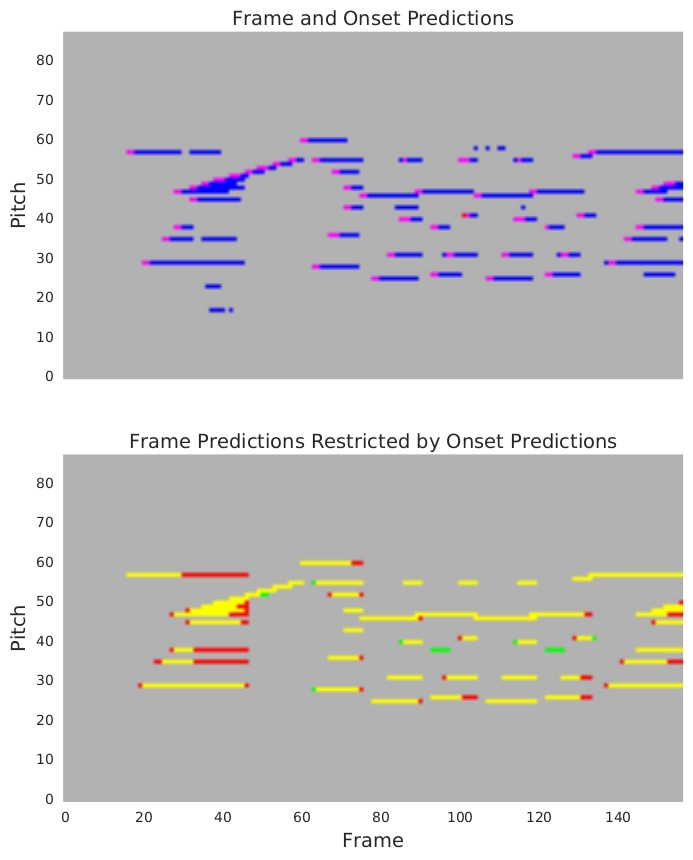
\includegraphics[width=0.6\textwidth,height=\textheight]{Images/frames.png}
\caption{MIDI transcriptions generated by Magenta's ``Onset Frames''
model.\newline\textit{Sourced from \href{https://magenta.tensorflow.org/onsets-frames}{Google's Magenta Blog}}}
\end{figure}

In the first image, blue indicates frame prediction, red indicates onset
prediction, and magenta indicates frame and onset prediction overlap.
There are several cases where the frame detector thinks there is a note
and the onset detector does not (notes that do not have a magenta block
at the beginning). Most of those frame detections are incorrect, which
illustrates the importance of removing notes that do not have a detected
onset. The second image shows the predictions after removing notes that
did not have a detected onset. Yellow indicates frame prediction and
ground truth overlap, green indicates an erroneous frame prediction, and
red indicates ground truth without a frame prediction
(\textit{image description also sourced from \href{https://magenta.tensorflow.org/onsets-frames}{Google's Magenta Blog}}).

Based on the transcriptions both create it is possible to compare them
qualitatively. Magenta's approach appears more committed in its choice
of notes and often more confident when it comes to timing due to its
training instilling a greater sense of tempo and structure in its
transcriptions. WaoN is sensitive and picks out many intricacies of a
song's dynamic range, but this often leads to the incorporation of more
false positives in terms of ghost notes (notes that should not be
present but are determined to be through frequency clashes, overtones
etc.).

Both seemed to be viable and offered slightly different versions of the
training data to be used in training the compositional models. Because
of this, it was decided that both should be used in order to augment the
dataset with additional files based on chosen raw audio. It is likely
that Magenta's model would be far superior to WaoN in fixed domain
transcriptions (i.e.~training the model on a dataset of ground truth
transcriptions of a certain genre before using it to transcribe more of
that genre, so that it might understand the `rules' of transcribing
genres other than classical more effectively). It is likely that in the
future applications such as WaoN will be largely eschewed in favour of
modern machine learning approaches similar to what has happened to the
field of Computer Vision over the past decade or so.

WaoN has numerous tuning parameters. The most regularly used were:

\begin{itemize}
\tightlist
\item
  \texttt{-n} for changing the sampling window from the input file,
  higher number results in fewer samples, as \texttt{-n} corresponds to
  the number of samples in a single step to be analysed.
\item
  \texttt{-c} allows the user to set the base-10 logarithm of the
  cut-off ratio upon which velocity of a note should be scaled,
  i.e.~lowering its value allows for weaker notes to be captured.
\item
  \texttt{-r} does the same but relative to the average velocity, this
  can be used to remove noisy notes from the outputted MIDI.
\end{itemize}

It was found that decreasing \texttt{-c} from its default and increasing
\texttt{-r} along with a relatively large sampling window \texttt{-n}
gave the best results with the fewest noisy notes and came closest to
emulating the original pieces. These outputs still often included many
more ghost notes than Magenta's outputs, but sometimes captured complex
structures that Magenta did not, contributing to the final decision to
use both approaches in tandem.

\hypertarget{gathering-a-training-corpus}{%
\subsection{Gathering a Training
Corpus}\label{gathering-a-training-corpus}}

WaoN and Magenta's ``Onset Frames'' model were used to convert a
personal library of ambient music containing approximately 1,400 pieces
spanning 180 hours into an author-created corpus of MIDI. This library's
raw audio was also fed into the sentimental analysis part of the code to
generate data on sentiment for each piece.

The model was also trained on classical music to make it more comparable
to existing offerings, and to reduce some of the issues regarding noisy
training data that creating an original corpus presented. The MAESTRO
dataset {[}\protect\hyperlink{ref-maestro2018}{19}{]} was used which is
potentially the largest of its kind, providing 1,200 pieces spanning 170
hours in \texttt{.wav} format alongside their ground truth MIDI files
(the audio \emph{and} MIDI were recorded together using an electronic
piano and microphones, so no MIDI transcription took place like the
processes described above, MAESTRO describes the ``perfect'' training
set for this kind of model). The raw audio could be used to analyse mood
which could then be associated with the MIDI files as before.

For evaluation in context of previous work, the four datasets JSB
Chorales, MuseData, Nottingham and Piano-Midi.de were also used as
discussed previously. These datasets did not include raw audio meaning
mood data was not able to be extracted from them; this was not an issue
as in order to remain relevant the sentiment part of each model's
architecture was effectively cut out when these datasets were used. This
was done to ensure the loss function values were comparable to previous
attempts which did not incorporate a mood representation.

\hypertarget{building-an-effective-representation-for-training}{%
\subsection{Building an Effective Representation for
Training}\label{building-an-effective-representation-for-training}}

After deciding on the raw training data to use, a schema was required to
represent the selected MIDI files in a tensor format so that they could
be used to train the model. MIDI was converted to tensors by iterating
through their files using the python package \texttt{mido}
{[}\protect\hyperlink{ref-mido}{47}{]}. In order to understand this
process, it is useful to consider the format of a MIDI file in that they
are a stream of messages containing:

\begin{itemize}
\tightlist
\item
  A message class, usually a \texttt{Note\ On} or \texttt{Note\ Off}
  event, but could also be \texttt{End\ of\ Track}, \texttt{Set\ Tempo}
  etc.
\item
  An affected note where applicable, in the range of 0 to 127, this is
  the standard range of MIDI as a format and represents around 10
  octaves on a piano.
\item
  A velocity associated with \texttt{Note\ On} events, ranging from 0 to
  127.
\item
  A tick value corresponding to the number of MIDI ticks that have
  passed since the \emph{previous} event.
\end{itemize}

Most existing solutions do \emph{not} have an effective means of
representing velocity in their training data. This was considered to be
an important factor when designing a representation, as much of what
makes music sound human comes from the dynamics that velocity can
contribute to a piece. Recent work by the Magenta team proposes one
method of incorporating velocity
{[}\protect\hyperlink{ref-performance-rnn-2017}{48}{]}, but their
research paper is still forthcoming, leading to the formulation of the
different method described below.

\texttt{mido} is used to iterate through MIDI events in order to
generate a sequence of numbers representing a MIDI file. In the
resulting sequence, the values 0 to 127 are reserved for notes, 128 to
159 are reserved for time and 160 to 192 are reserved for velocity. Time
and velocity are packed into bins for performance reasons rather than
trying to attempt to represent all possible times and velocity levels;
32 bins were deemed to be sufficient. A new number is appended to the
sequence first for the time when an event occurs, then for the velocity
of said event if it concerns a played note, and finally a number
corresponding the note value itself is added. If a time exceeds the
length of time represented by the \(32^{nd}\) time bin, additional
numbers are appended to the sequence representing the remaining time.

A MIDI file containing the following events would be converted as below:

\[\begin{gathered}
\text{(Note On Event, Note = 55, Velocity = 90, Tick = 831)} \\
\text{(Note On Event, Note = 67, Velocity = 85, Tick = 3)}\\
\cdots\\
\text{Becomes : } [159, 182, 55, 181, 67, \dots]
\end{gathered}\]

Note that a tick value of 3 is not sufficient to warrant the inclusion
of another time-bucketed event meaning that there is no `gap' between
the playing of notes 55 and 67 in this representation. Ticks can be
converted to some number of milliseconds meaning that these small
changes in time resolution through binning are imperceptible to us as
listeners. It was relatively simple to test the efficacy of this
representation by converting from MIDI and back and then comparing the
input and output MIDI files. These comparisons were satisfactory for the
purposes of this project, with no perceivable difference or loss of
precision through conversion.

Once the training data is in this form it is randomly sampled into equal
length sequences for training purposes. The resulting array
representations are one hot encoded to turn them into two-dimensional
tensors before being fed into the model in batches. This leads to each
element of an input sequence having the dimension:

\[\begin{aligned}
D_{\text{input}} &= \text{Number of Possible MIDI Notes} + \text{Buckets for time} + \text{Buckets for Velocity}\\
&= 128 + 32 + 32\\
&= 192
\end{aligned}\]

The above corresponds to the dimension of a single event vector in a
training sequence. In practice, the three-dimensional tensors created
through batching and random sampling of training data have the following
dimension:

\[\text{Batch Size} \times \text{Training Sequence Length} \times D_{\text{input}}\]

A mood vector is inputted separately and eventually merged with the
training sequences by the model using a linear unsqueeze operation to
distribute it across the first layer.

\hypertarget{sentiment-analysis}{%
\section{Sentiment Analysis}\label{sentiment-analysis}}

In order to satisfy the requirements of the project regarding sentiment,
it was necessary to first extract the sentiment from each component of
the training data corpus and then formulate a means of attaching this
sentiment to the representation of the training data to be fed into the
model during training.

Much of the technical work regarding extraction of sentiment from audio
follows the work done by the DeepSent project
{[}\protect\hyperlink{ref-deepsent}{44}{]}. This code was used as a
basis upon which a vector of mood values could be generated
automatically for each element of the chosen datasets and then
associated with the MIDI files to be used in training. Sentiment is
measured with respect to an arousal-valence emotional model known as the
Circumplex model
{[}\protect\hyperlink{ref-russell1980circumplex}{49}{]}, with values
being determined for both axes of arousal and valence.

\begin{figure}
\centering
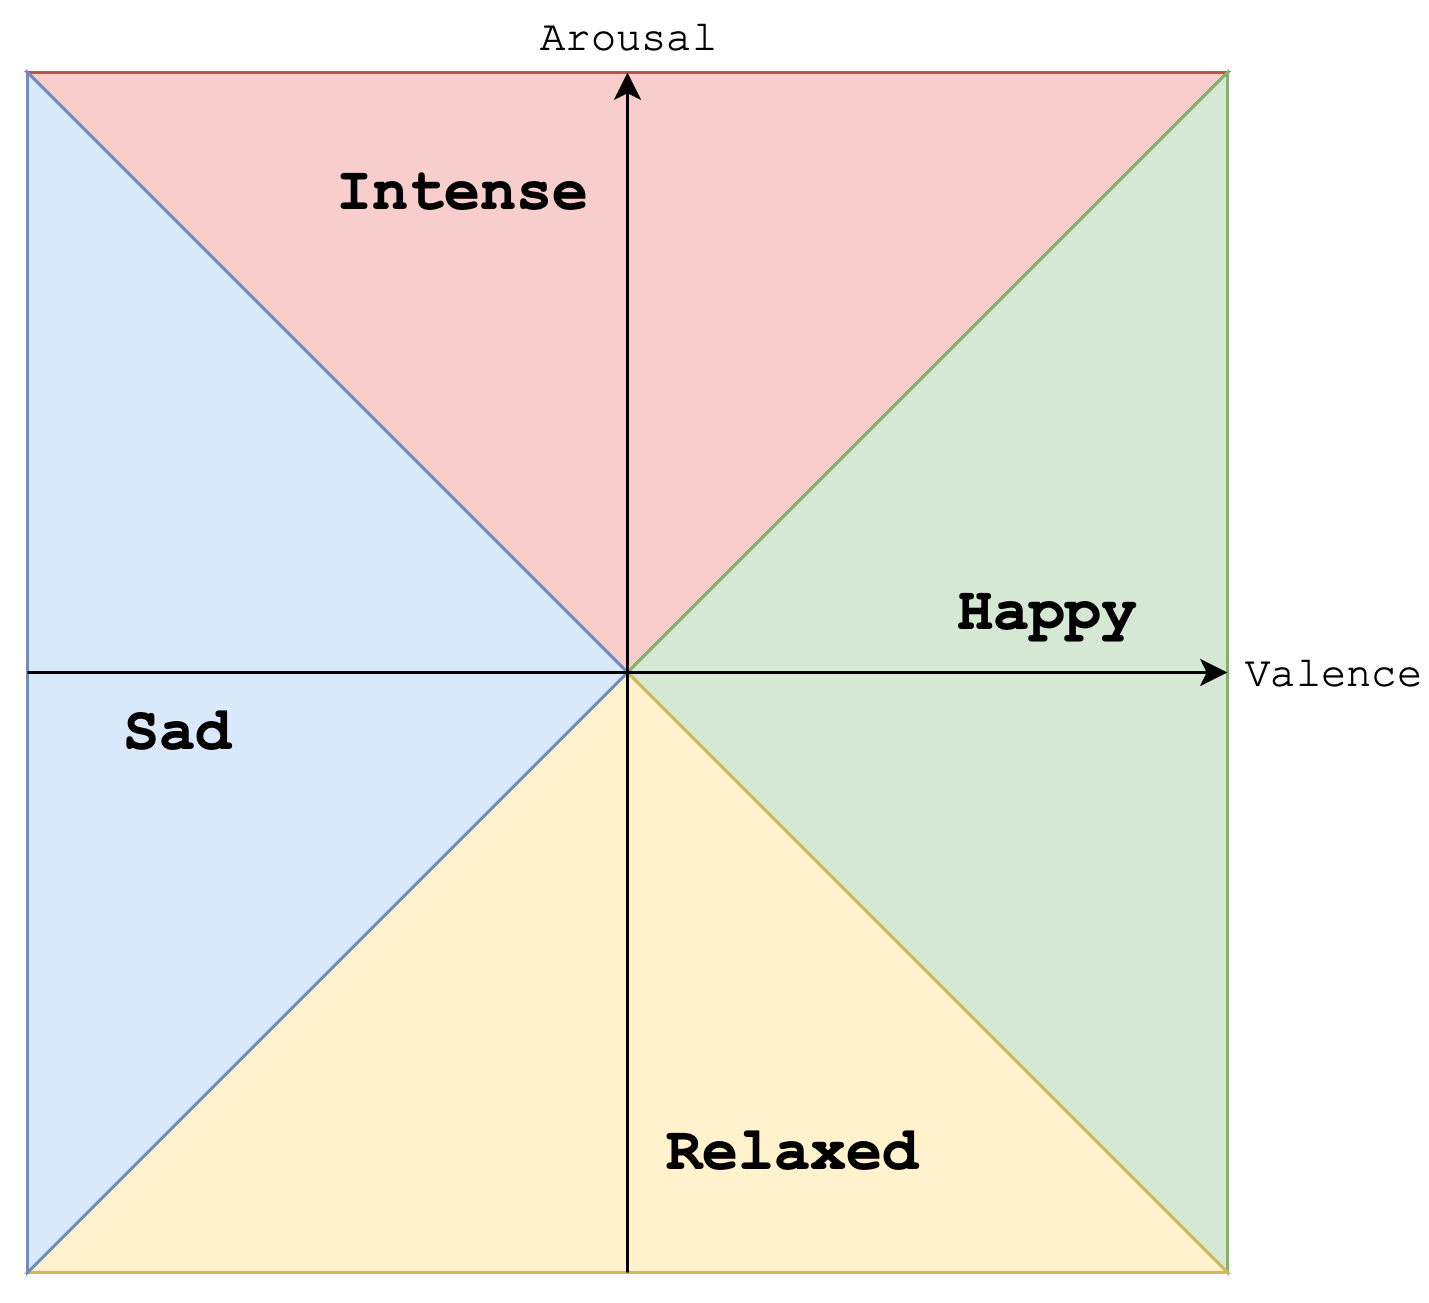
\includegraphics[width=0.6\textwidth,height=\textheight]{Images/circumplex.png}
\caption{Two-dimensional representation of the Circumplex model with
descriptive labels plotted on the resulting plane.}
\end{figure}

In this context, arousal refers to the perceived intensity of a piece;
ranging from a relaxed or somewhat lethargic feeling to a more intense
and excited stimulation. Valence is a spectrum of a piece's incited
effect on a listener's level of happiness or sadness. This model was
chosen as it captured much of the emotional impact of music in a
parsimonious way; trying to apply higher dimensional models of emotion
tended to lead to less meaningful predictions by the models. Values for
both axes were estimated and ratios calculated to fulfil three ratio
values regarding each axis. The ratios are calculated as shown below
following predictions made by the models:

\[\begin{aligned}
S_A &= \{\text{Scores assigned to each input by the arousal regressor model}\} \\
\text{Arousal Intense Ratio } &= \frac{\sum_{S_A} \mathbbm{1}_{\text{Score}> 2}}{|S_A|} \\
\text{Arousal Relaxing Ratio } &= \frac{\sum_{S_A} \mathbbm{1}_{\text{Score}< 1}}{|S_A|} \\
\text{Arousal Mid Ratio } &= 1 - (\text{Arousal Intense Ratio} + \text{Arousal Relaxing Ratio})
\end{aligned}\] \[\begin{aligned}
S_V &= \{\text{Scores assigned to each input by the valence regressor model}\} \\
\text{Valence Happy Ratio } &= \frac{\sum_{S_V} \mathbbm{1}_{\text{Score}> 2}}{|S_V|} \\
\text{Valence Sad Ratio } &= \frac{\sum_{S_V} \mathbbm{1}_{\text{Score}< 1}}{|S_V|} \\
\text{Valence Neutral Ratio } &= 1 - (\text{Valence Happy Ratio} + \text{Valence Sad Ratio}) \\
\end{aligned}\]

In both cases it can be seen that ratios are calculated through taking
the top and bottom few scores and calculating the ratio of each above
and below boundaries which were formulated through testing and with
respect to the original work. It is worth noting that all scores fall
between a range of 0 and around 5, but extreme values are clipped to 3
as they are often spurious.

These scores represent an abstract summing of numerical results from the
applied signal processing techniques. The important thing is their
relation to a calculated mean (falling within the mid / neutral ratios)
and to each other.

\hypertarget{implementing-signal-processing-techniques-and-returning-the-results-in-a-usable-form}{%
\subsection{Implementing Signal Processing Techniques and Returning the
Results in a Usable
Form}\label{implementing-signal-processing-techniques-and-returning-the-results-in-a-usable-form}}

Each piece to be analysed is trimmed of its start and end (which are
likely to be sparse and potentially irregular in terms of their content
when compared to the main body of a piece occurring around its midpoint)
to leave the middle 70\% of the data. This raw data is then windowed
into 5-second long frames of samples, with a step of 0.5 seconds between
the starting points of each (such that there is overlap between frames).
Within each of these there is then a further decomposition into 25ms
sub-frames that are transformed into an array of Mel-frequency cepstral
coefficients (MFCCs) {[}\protect\hyperlink{ref-logan2000mel}{50}{]}.

The matrices representing the MFCCs for each sub-frame are then
flattened and fed into a 3-layer neural network regressor. The neural
networks associate patterns common within certain moods based upon what
was learnt from numerous large datasets used for training these models.
More details of this training process are available in discourse
provided by the author of DeepSent. MFCCs represent features of audio
important for the identification of sentiment but also have been applied
in the areas of transcription and speech recognition.

The scores from the regressors are used to calculate the aforementioned
ratios which are then packed into a six-item vector and associated with
each of the training MIDI files to be loaded during training.
Thresholding as a means of segmentation was implemented by setting all
ratios greater than 50 to 1 and those below 50 to 0. This offered
computational improvements but potentially slightly decreased the
effectiveness of the mood transfer to training pieces. Due to the
subjectivity of this part of the output, it was hard to assess which
approach was more effective in capturing mood and so the simpler, less
computationally intense thresholding option was chosen. This resulted in
a six-element \emph{binary} vector representing mood associated with
each item in the training corpus.

\hypertarget{creating-a-recurrent-model-for-musical-composition}{%
\section{Creating a Recurrent Model for Musical
Composition}\label{creating-a-recurrent-model-for-musical-composition}}

After formulating an effective representation and transcription
pipeline, it is now appropriate to introduce some concepts in neural
networks and the research and theory which leads to the finalised model
architectures presented in this report.

\hypertarget{recurrent-neural-networks}{%
\subsection{Recurrent Neural Networks}\label{recurrent-neural-networks}}

Perhaps the most common form of artificial neural network is the
\emph{feedforward} network which utilises connected layers of neurons
and activation functions to approximate different functions through the
learning of parameters and weights between connections. Their main
limitations in this context are that they require their inputs to be of
a fixed dimension and thus are not well suited to dynamic data of
varying size such as a sequence \((x_t)_{1\le t\le T}\) of time stepped
note states representing a composition where \(T\) is the length of the
piece.

It is assumed that this type of sequential data has some system of
dependence on its prior and potentially future elements and so it would
not be appropriate to assume independence and simply input each element
of a temporal sequence into a feedforward network during training. It
can clearly be seen by observing musical data and considering knowledge
of musical theory that input at each time step is likely to be dependent
on other time steps (e.g.~compositions have an associated and consistent
\emph{key} which may be inferred by chords and notes present throughout
the piece).

This class of situations led to the development of \textbf{recurrent
neural networks} which introduce recurrent connections between layers
over a temporal dimension allowing the network to exhibit dynamic
behaviour over time. Their evolution over time depends on the inputs as
well as its previous / current state. They could be considered to be an
evolution of hidden Markov models
{[}\protect\hyperlink{ref-baum1966}{51}{]} but with the addition of a
distributed state allowing for more complex and dynamic behaviours to be
captured in a computationally effective manner.

It is now possible to provide some notation specific to this project
regarding RNNs. A training input is defined
\protect\hyperlink{buildinganeffectiverepresentationfortraining}{as
before}, with the vector corresponding to the sequence at time \(t\)
denoted as \(x_t\in \{0,1\}^{D_{\text{input}}}\). At each time step, a
layer's input \(x_t\) and its previous state \(h_{t-1}\) are used to
calculate a new value \(h_t\) for each hidden layer
\(h\in\{\text{Hidden Layers}\}\) and also inform the outputs for that
time step \(y_t\). Mathematically, this recurrent relationship can be
formulated as follows:

\[\begin{aligned}
h_t &= \phi(W_{xh} x_t + W_{hh} h_{t-1} + b_{xh}) \\
y_t &= \phi(W_{hy} h_t + b_{hy})
\end{aligned}\]

Where:

\begin{itemize}
\tightlist
\item
  \(\phi\) is the chosen element-wise activation function for the
  network.
\item
  \(W_{xy}\) represents the weight parameters between layers \(x\) and
  \(y\), these weight parameters are learned using backpropagation
  through time (BPTT)
  {[}\protect\hyperlink{ref-werbos1990backpropagation}{52}{]}.
\item
  \(b_{xy}\) is the bias parameter between layers \(x\) and \(y\) also
  adjusted during training via BPTT or a similar algorithm.
\end{itemize}

In this case and all proceeding cases, where there are multiple hidden
layers, assume that the input for the \(n^{\text{th}}\) layer
\(h^{(n)}_t\) is \(x_t = h^{(n-1)}_t\).

\begin{figure}
\centering
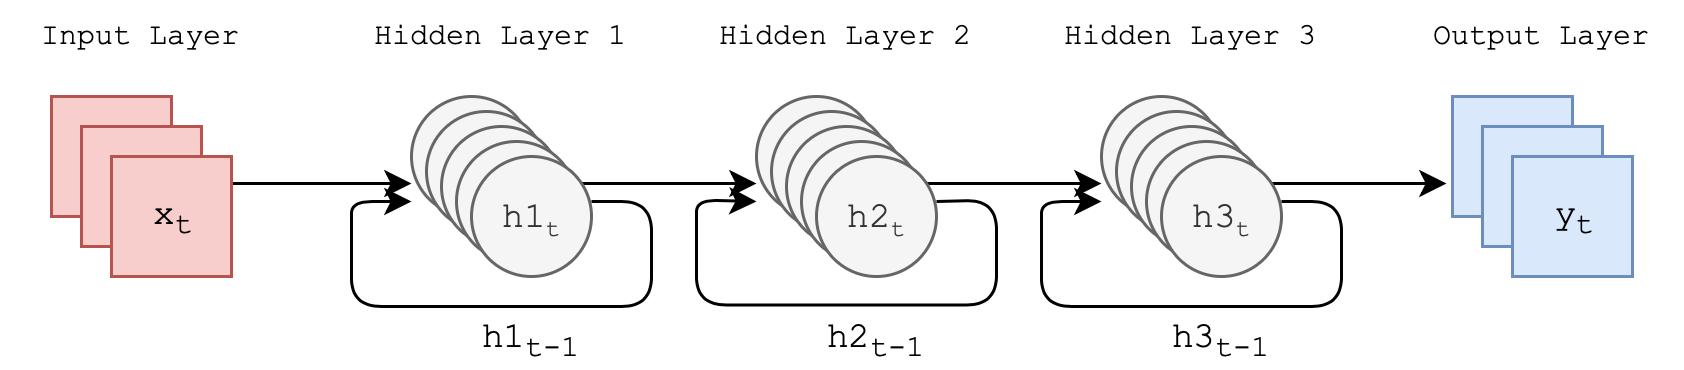
\includegraphics{Images/rnn.png}
\caption{Recurrent connections between the hidden layers of an RNN.}
\end{figure}

This process is illustrated in the figure above and can be explained by
considering that at the start of the process all weights and activations
are initialised to some value. At each time step following this, the new
activations for each hidden layer are calculated using a combination of
the current time step's input and that layer's previous activations.
This process highlights the possibility of unrolling an RNN into a DAG
(directed acyclic graph) representation as shown in the figure below:

\begin{figure}
\centering
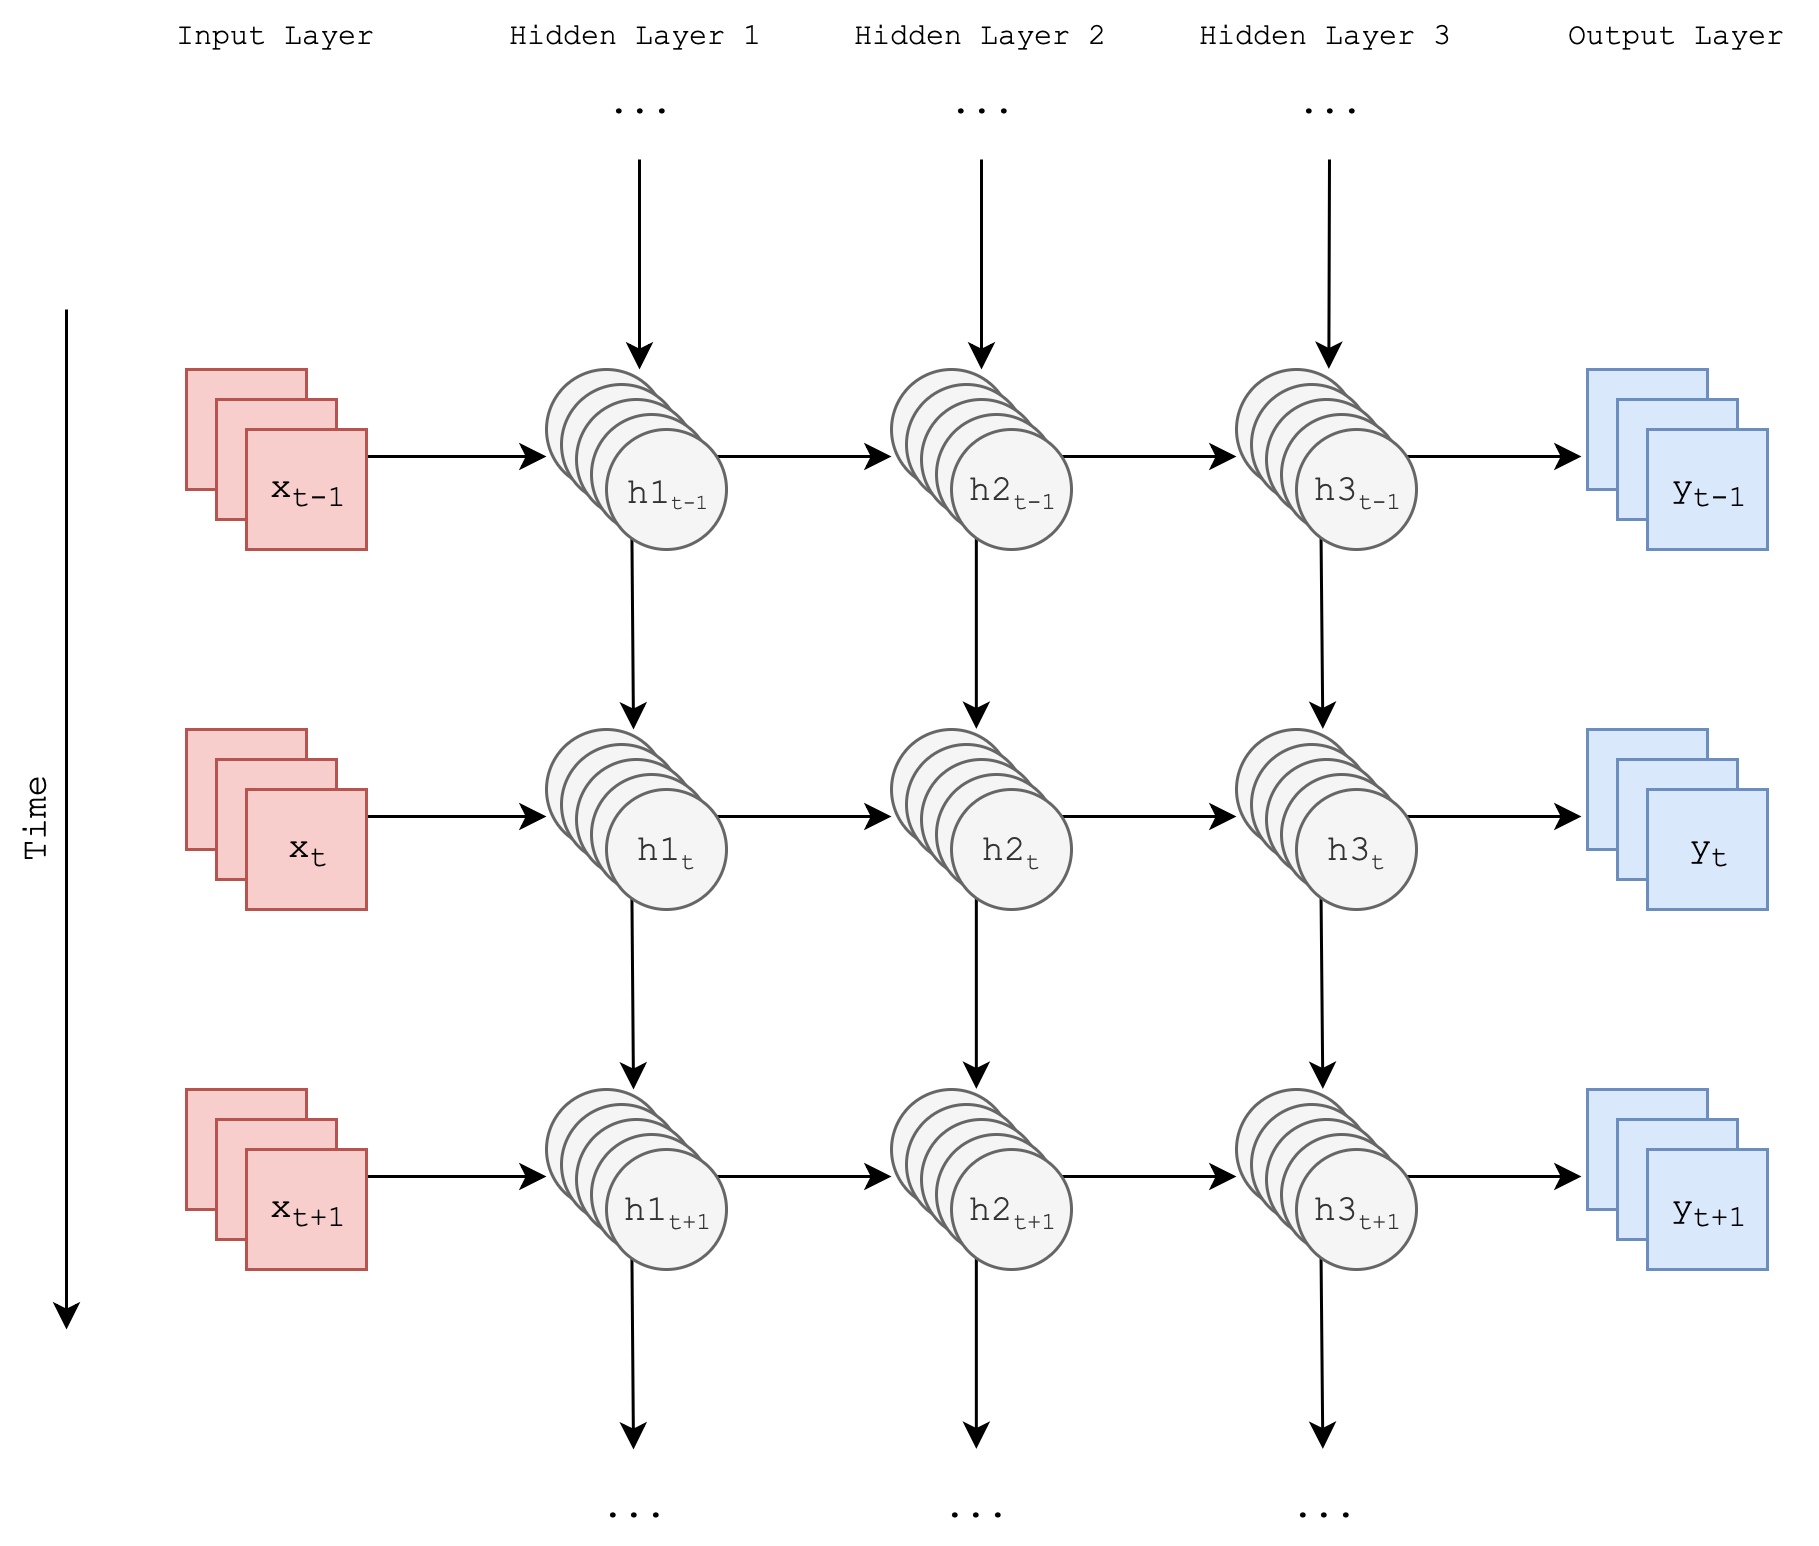
\includegraphics{Images/unrolledrnn.png}
\caption{Another illustration of a basic RNN, with its recurrent
connections unrolled along the time axis to result in a DAG.}
\end{figure}

The potentially most important property of this class of network is
their \emph{time invariance}, in that at a given time step the networks'
activations and learned properties can all be considered relative to
previous time steps. The activations, weights and biases at one time
step influence the next and potentially all future time steps, meaning
dependencies can be learned over time. The ability to recurrently input
data into the network is the clear reason for its usage in this context
over traditional feedforward networks.

\hypertarget{issues}{%
\subsubsection{Issues}\label{issues}}

Recurrent neural networks such as these often learn through the Back
Propagation Through Time algorithm
{[}\protect\hyperlink{ref-werbos1990backpropagation}{52}{]} (or some
variant of it), this is an algorithm which roughly can be described as
propagating error back through a network's graph by traversing the
connections made across time steps in reverse order and updating the
parameters in order to improve a model's specified loss / error metric.
To do this, it calculates gradients from which new parameters for the
network's units may be calculated; it utilises differentials and
integration to do this as error is distributed backwards throughout the
network's units.

This algorithm presents a number of problems, not least that it requires
architectures to be made almost entirely of differentiable components in
order for backpropagation optimisation to be applied. The main issues
encountered for recurrent neural networks are with respect to the
calculation of vanishing and exploding gradients
{[}\protect\hyperlink{ref-pascanu2012understanding}{53}{]} during this
optimisation which occurs when small or large values are propagated back
in a graph with a huge number of connections and parameters (as
recurrent networks in this problem space often have).

There are numerous proposals for solving these issues and many were
tested or applied to the final models; one common example is for steps
to be made during the training process to clip any outlier gradient
values.

Despite their time invariance and flexibility in terms of the dimension
of their inputs, RNNs also lack long-term coherence meaning they often
fail when complex dependencies are built up and different temporal
structures must be captured. They are very susceptible to this issue of
exploding or vanishing gradients over time due to repeated and recurrent
backpropagation; tiny or large values will often compound and be
multiplied together leading to the network getting stuck or
significantly slowing its learning.

These issues have inspired a number of variant units replacing the
traditional RNN node which aim to mitigate these problems and thus form
the basis of most current approaches to musical composition. Through
considerable research
{[}\protect\hyperlink{ref-lipton2015critical}{54}{]}--{[}\protect\hyperlink{ref-dey2017gate}{57}{]},
it was decided that LSTMs and GRUs should be trialled against each other
as part of this project's model architecture due to their pre-eminent
position in this area as promising solutions to the issues outlined
here. As well as aiming to mitigate these issues, they aid in capturing
long-term dependencies through the careful control of data flowing
through a network of these units over time.

\hypertarget{long-short-term-memory-recurrent-units}{%
\subsubsection{Long Short-Term Memory Recurrent
Units}\label{long-short-term-memory-recurrent-units}}

The LSTM unit was first proposed in 1999
{[}\protect\hyperlink{ref-gers1999learning}{7}{]}, though the version
formulated here includes some improvements based on more recent research
{[}\protect\hyperlink{ref-greff2017lstm}{55}{]},
{[}\protect\hyperlink{ref-sak2014long}{58}{]},
{[}\protect\hyperlink{ref-zebin2018human}{59}{]}, the most notable
addition is that of the \emph{forget gate}. LSTMs introduce a means of
allowing long-term dependencies to be captured by RNNs through
introducing three `gates' which each interact with a cell memory state
\(c_t\) and previous hidden activations passed through time:

\begin{itemize}
\tightlist
\item
  The \textbf{forget gate} is a scaling factor
  \[f_t = \sigma(W_{if} x_t + b_{if} + W_{hf} h_{t-1} + b_{hf})\] where
  \(\sigma(x) = 1 / (1 + e^{-x})\) is the sigmoid function; its values
  fall in \([0,1]\) and control the extent to which the previous cell
  memory state \(c_{t-1}\) is kept / forgotten.
\item
  The \textbf{input gate} is a scaling factor
  \[i_t = \sigma(W_{ii} x_t + b_{ii} + W_{hi} h_{t-1} + b_{hi})\] where
  the terms are self-explanatory; its values fall in \([0,1]\) and
  control the extent to which the new candidate memory state \(c^*_t\)
  flows into the unit.
\item
  The \textbf{output gate} is a scaling factor
  \[o_t = \sigma(W_{io} x_t + b_{io} + W_{ho} h_{t-1} + b_{ho})\] where
  the terms are self-explanatory; its values fall in \([0,1]\) and
  control the extent to which the new memory state \(c_t\) is used to
  compute the new activation \(h_t\).
\end{itemize}

The candidate memory state \(c^*_t\) is calculated as
\[c^*_t = \tanh(W_{ic^*} x_t + b_{ic^*} + W_{hc^*} h_{t-1} + b_{hc^*})\]
which can then be multiplied element-wise with the input gate scaling
factor and added with the result of the forget gate scaling factor's
element-wise multiplication with the previous memory state:
\[c_t = f_t \odot c_{t-1} + i_t \odot c^*_t\] Finally, the new / current
hidden activation state can be found as: \[h_t = o_t \odot \tanh(c_t)\]
All of these weights and bias parameters are updated during training via
backpropagation as before and initialised in this instance from the
uniform distribution:
\[U(-\sqrt{k}, \sqrt{k}),\quad k = \frac{1}{\text{Hidden Layer Size}}\]

The diagram below illustrates the LSTM and the flow of data through it
diagrammatically; it may be helpful to imagine this structure chained in
sequence horizontally in order to understand the flow of time in a
network composed of these units. Recurrent connections through time
exist between the output and input of these units when present in a
neural network, as in the simple RNN illustrated previously.

\begin{figure}
\centering
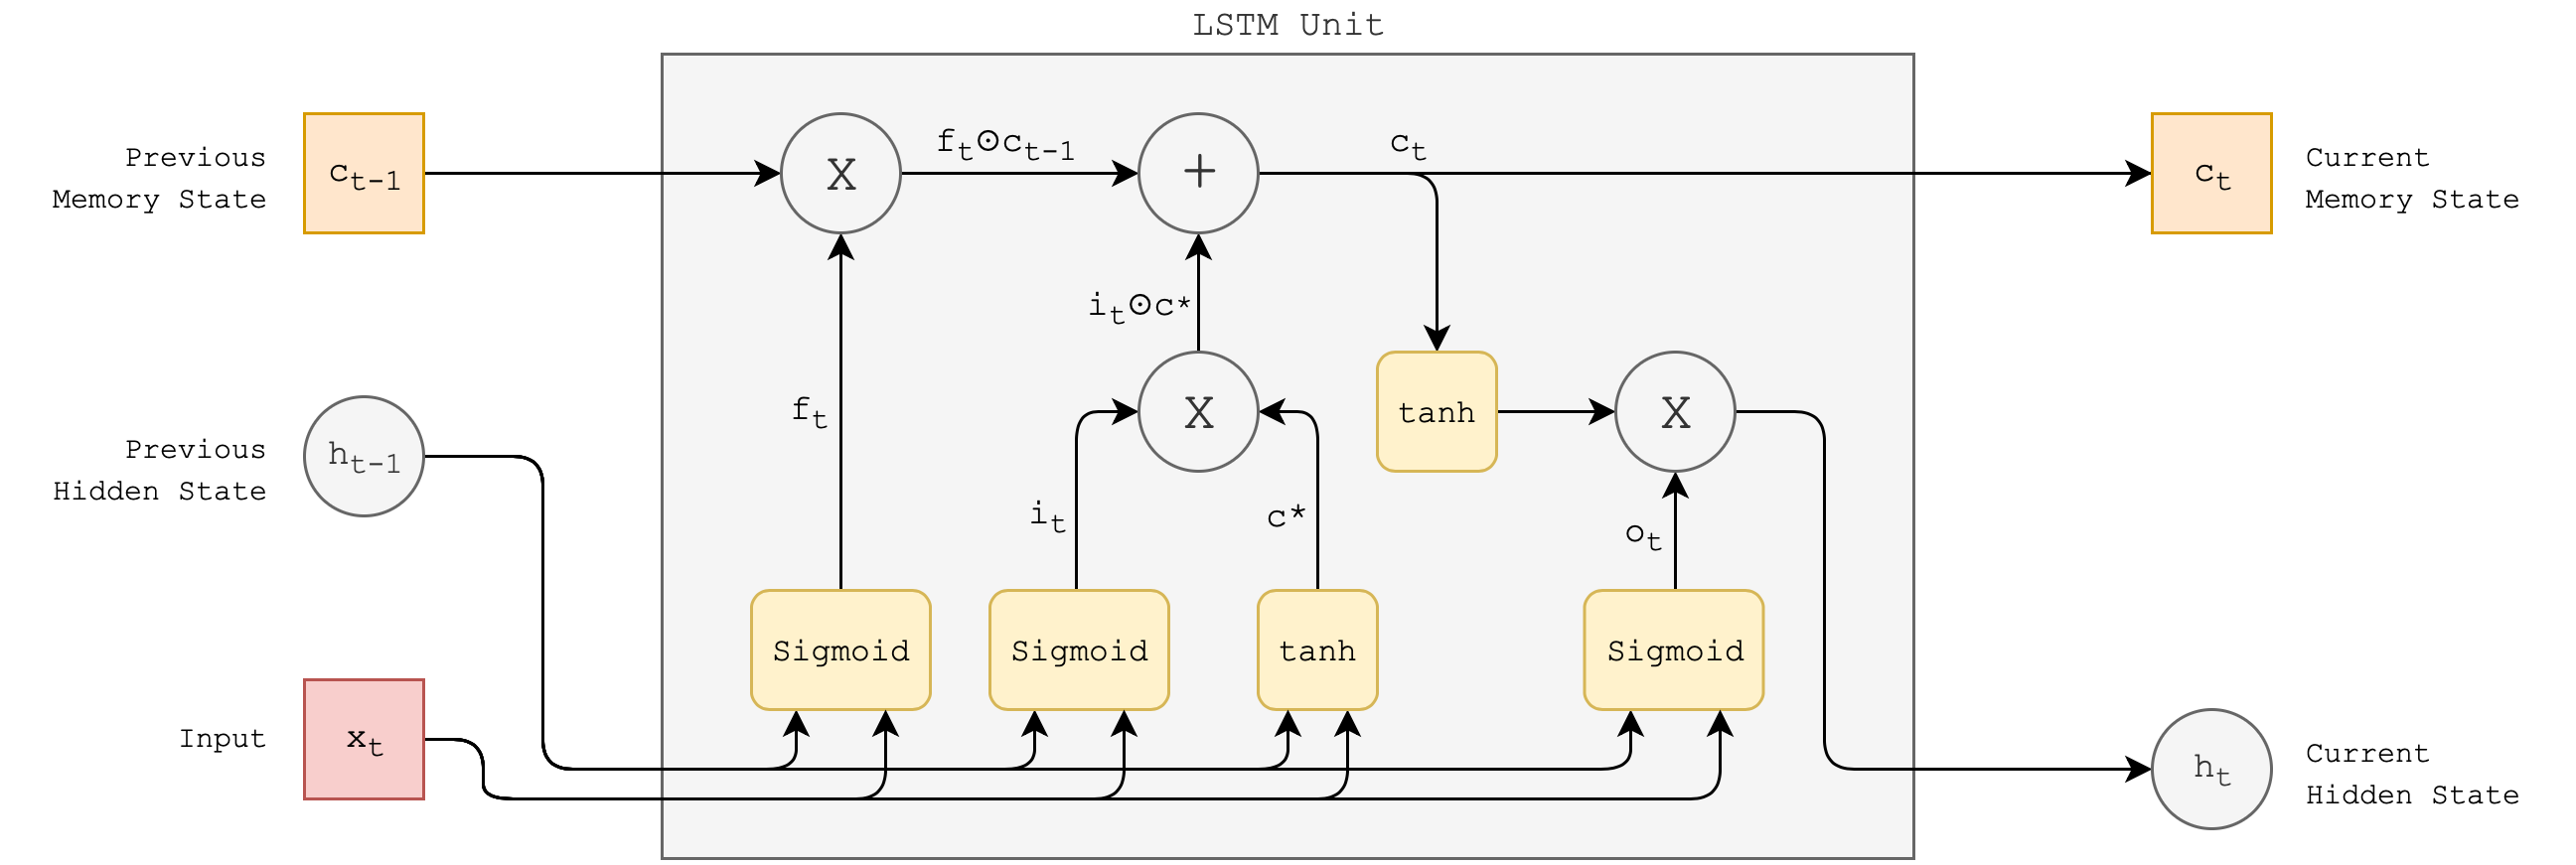
\includegraphics{Images/lstm.png}
\caption{The inner structure of a Long Short-Term Memory Unit, visually
representing its forget, input and output gates and the flow of data
through the unit.}
\end{figure}

Note that there are many small variations on the LSTM concept; the
mathematical formulation was written here in context of PyTorch's
implementation {[}\protect\hyperlink{ref-pytorchlstm}{60}{]} and the
figure reflects this.

\hypertarget{gated-recurrent-units}{%
\subsubsection{Gated Recurrent Units}\label{gated-recurrent-units}}

The GRU was first proposed in 2014
{[}\protect\hyperlink{ref-cho2014learning}{34}{]}. It offers a similar
set of operations to try and mitigate the aforementioned issues with
RNNs. It does so by introducing two `gates' in a slightly simpler
configuration to the LSTM:

\begin{itemize}
\tightlist
\item
  The \textbf{reset gate} is a scaling factor
  \[r_t = \sigma(W_{ir} x_t + b_{ir} + W_{hr} h_{t-1} + b_{hr})\] where
  \(\sigma(x) = 1 / (1 + e^{-x})\) is the sigmoid function; its values
  fall in \([0,1]\) and control the extent to which the previous cell
  memory state \(c_{t-1}\) is kept / forgotten such that the unit could
  essentially be reset to consider only its recent inputs in extreme
  cases.
\item
  The \textbf{update gate} is a scaling factor
  \[z_t = \sigma(W_{iz} x_t + b_{iz} + W_{hz} h_{t-1} + b_{hz})\] where
  the terms are self-explanatory; its values fall in \([0,1]\) and
  control the extent to which the unit's activation is updated.
\end{itemize}

The candidate activation state \(h_t^*\) is calculated as
\[h_t^* = \tanh(W_{ih^*} x_t + b_{ih^*} + r_t (W_{hh^*} h_{t-1} + b_{hh^*}))\]
which can then be used in calculating the new / current activation via a
linear interpolation of the candidate activation and the previous
activation: \[h_t = h_{t-1} (1 - z_t) + h_t^* z_t\]

The diagram below illustrates the GRU and the flow of data through it
diagrammatically.

\begin{figure}
\centering
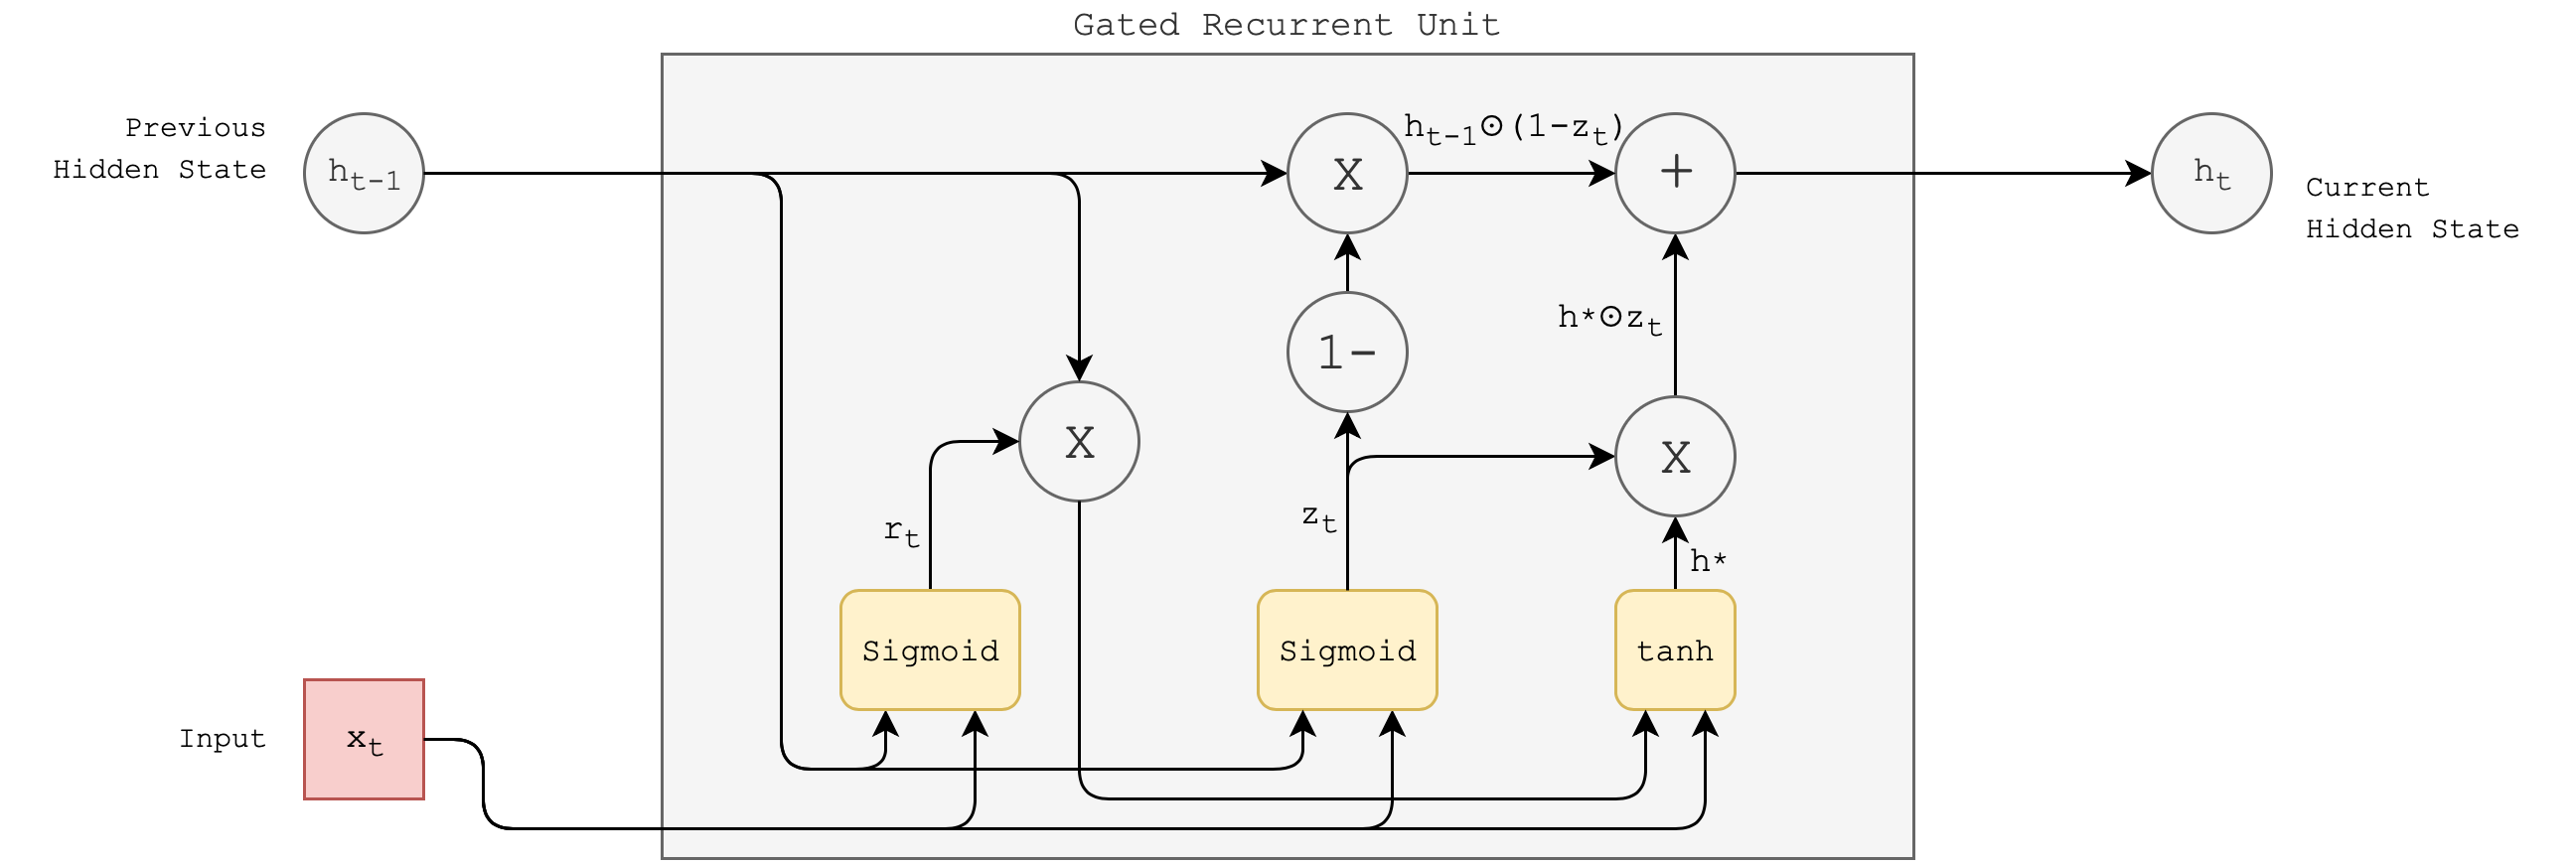
\includegraphics{Images/gru.png}
\caption{The inner structure of a Gated Recurrent Unit, visually
representing its reset and update gates and the flow of data through the
unit.}
\end{figure}

Note that there are many small variations on the GRU concept; the
mathematical formulation was written here in context of PyTorch's
implementation {[}\protect\hyperlink{ref-pytorchgru}{61}{]} and the
figure reflects this.

Both of these units' gates offer provable improvements over their
``vanilla'' RNN counter-parts
{[}\protect\hyperlink{ref-chung2014empirical}{62}{]} by exposing a
greater number of learnable parameters to control the information
flowing through the network over time. This gives the network the
opportunity to be more selective in the dependencies it builds by
minimising or maximising certain states throughout training. These
additional parameters introduce greater complexity into the models but
this complexity is usually justified, especially in scenarios where RNNs
have been shown to suffer as they do in musical composition.

\hypertarget{dilation}{%
\subsection{Dilation}\label{dilation}}

The concept of dilation was first proposed in the context of
convolutional neural networks
{[}\protect\hyperlink{ref-yu2015multi}{63}{]} for image analysis and
semantic segmentation; this work was discovered during research for a
\protect\hyperlink{sentimentalinputfromimages}{potential extension} of
this project. The main concept is to aggregate information at different
contextual scalings without losing resolution by exploding a kernel's
considered neighbourhood around a central pixel / element. This is done
to increase the likelihood of discovering pattern structures at
different resolutions within an input as well as increasing the area of
an image or input which can be considered through a small number of
steps. Some other attempts to capture these structural characteristics
have been made but usually involve restrictions placed on the outputs of
a model rather than being ingrained into the architecture of the model
itself as has been attempted here.

Dilation offers an alternative to other techniques often relying on
down-sampling which sacrifice resolution rather than considering
different contexts at full resolution. This technique has shown to be
very effective in aiding dense prediction problems (predicting labels
for each pixel in an image, or with respect to this project's proposed
equivalence of predicting on or off states for each note on the piano
over a series of time steps). Deepmind researchers applied a similar
approach within their own convolutional network for WaveNet which is the
first documented use of dilation in the musical composition domain
{[}\protect\hyperlink{ref-oord2016wavenet}{10}{]}. Their results found
that the addition of dilation increased the accuracy and effectiveness
of their model.

\begin{figure}
\centering
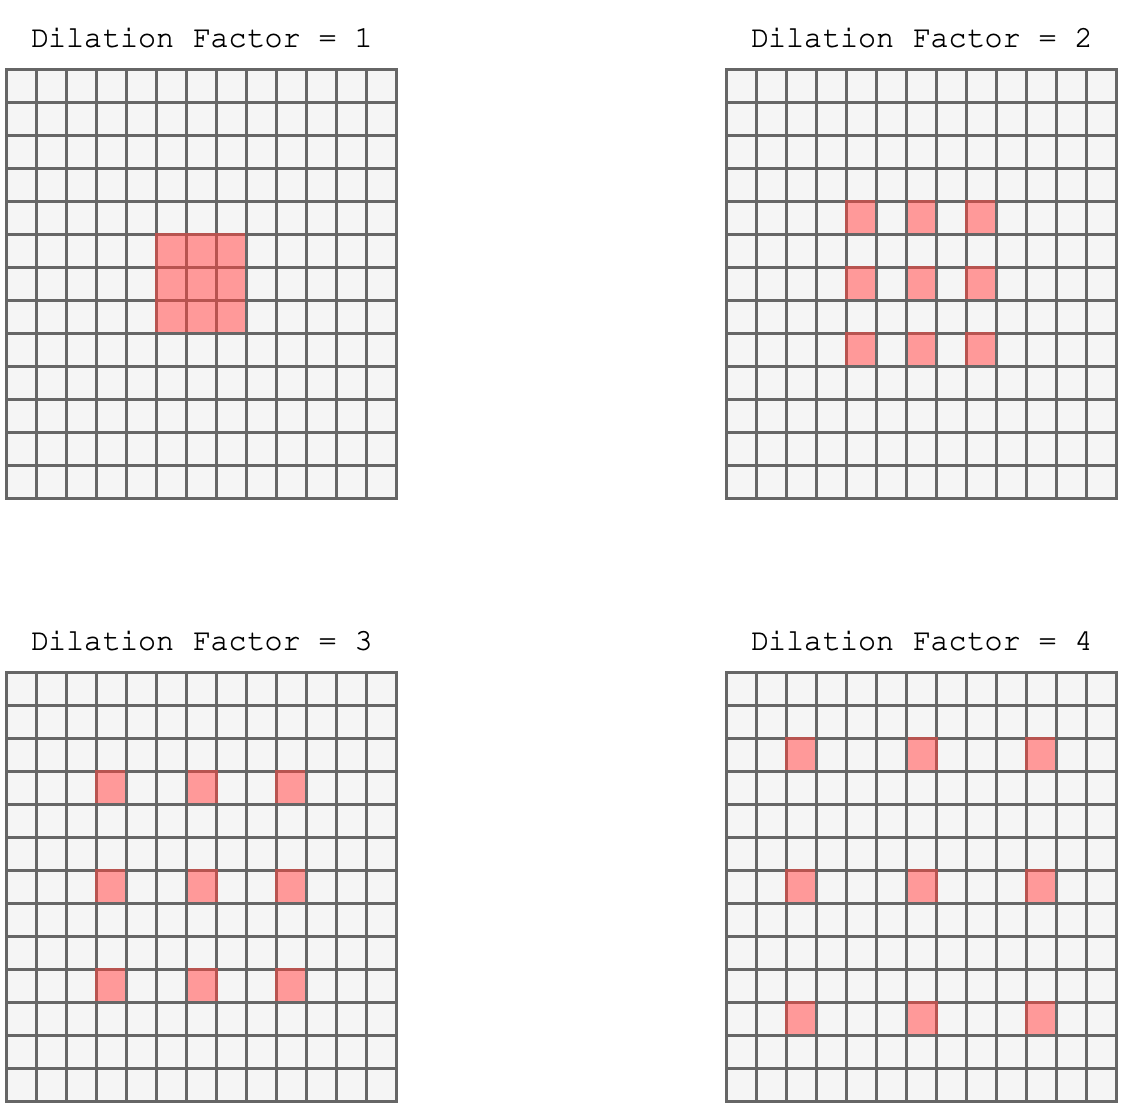
\includegraphics[width=0.7\textwidth,height=\textheight]{Images/dilation2d.png}
\caption{Different dilation factors illustrated on a 2-dimensional
input.}
\end{figure}

A paper was published linking this concept with recurrent neural
networks in 2017 {[}\protect\hyperlink{ref-chang2017dilated}{64}{]}.
This paper forms the basis for the justification of using dilation in
the model present in this project; this project's compositional model is
potentially the first use of dilated recurrent neural networks in the
musical composition domain. Dilation in the context of an RNN involves
skipping recurrent connections rather than skipping pixels in an input
image. Different layers can exhibit different dilation factors to
capture dependencies at different temporal resolutions and localities.
Dilation's purpose in the scenario of musical composition is to allow a
model to learn at multiple temporal resolutions and capture the
complexities of music that exist naturally through its formulation in
terms of half and double length notes, beats, bars etc. This immediately
lends itself to dilation factors of increasing powers of 2.

\begin{figure}
\centering
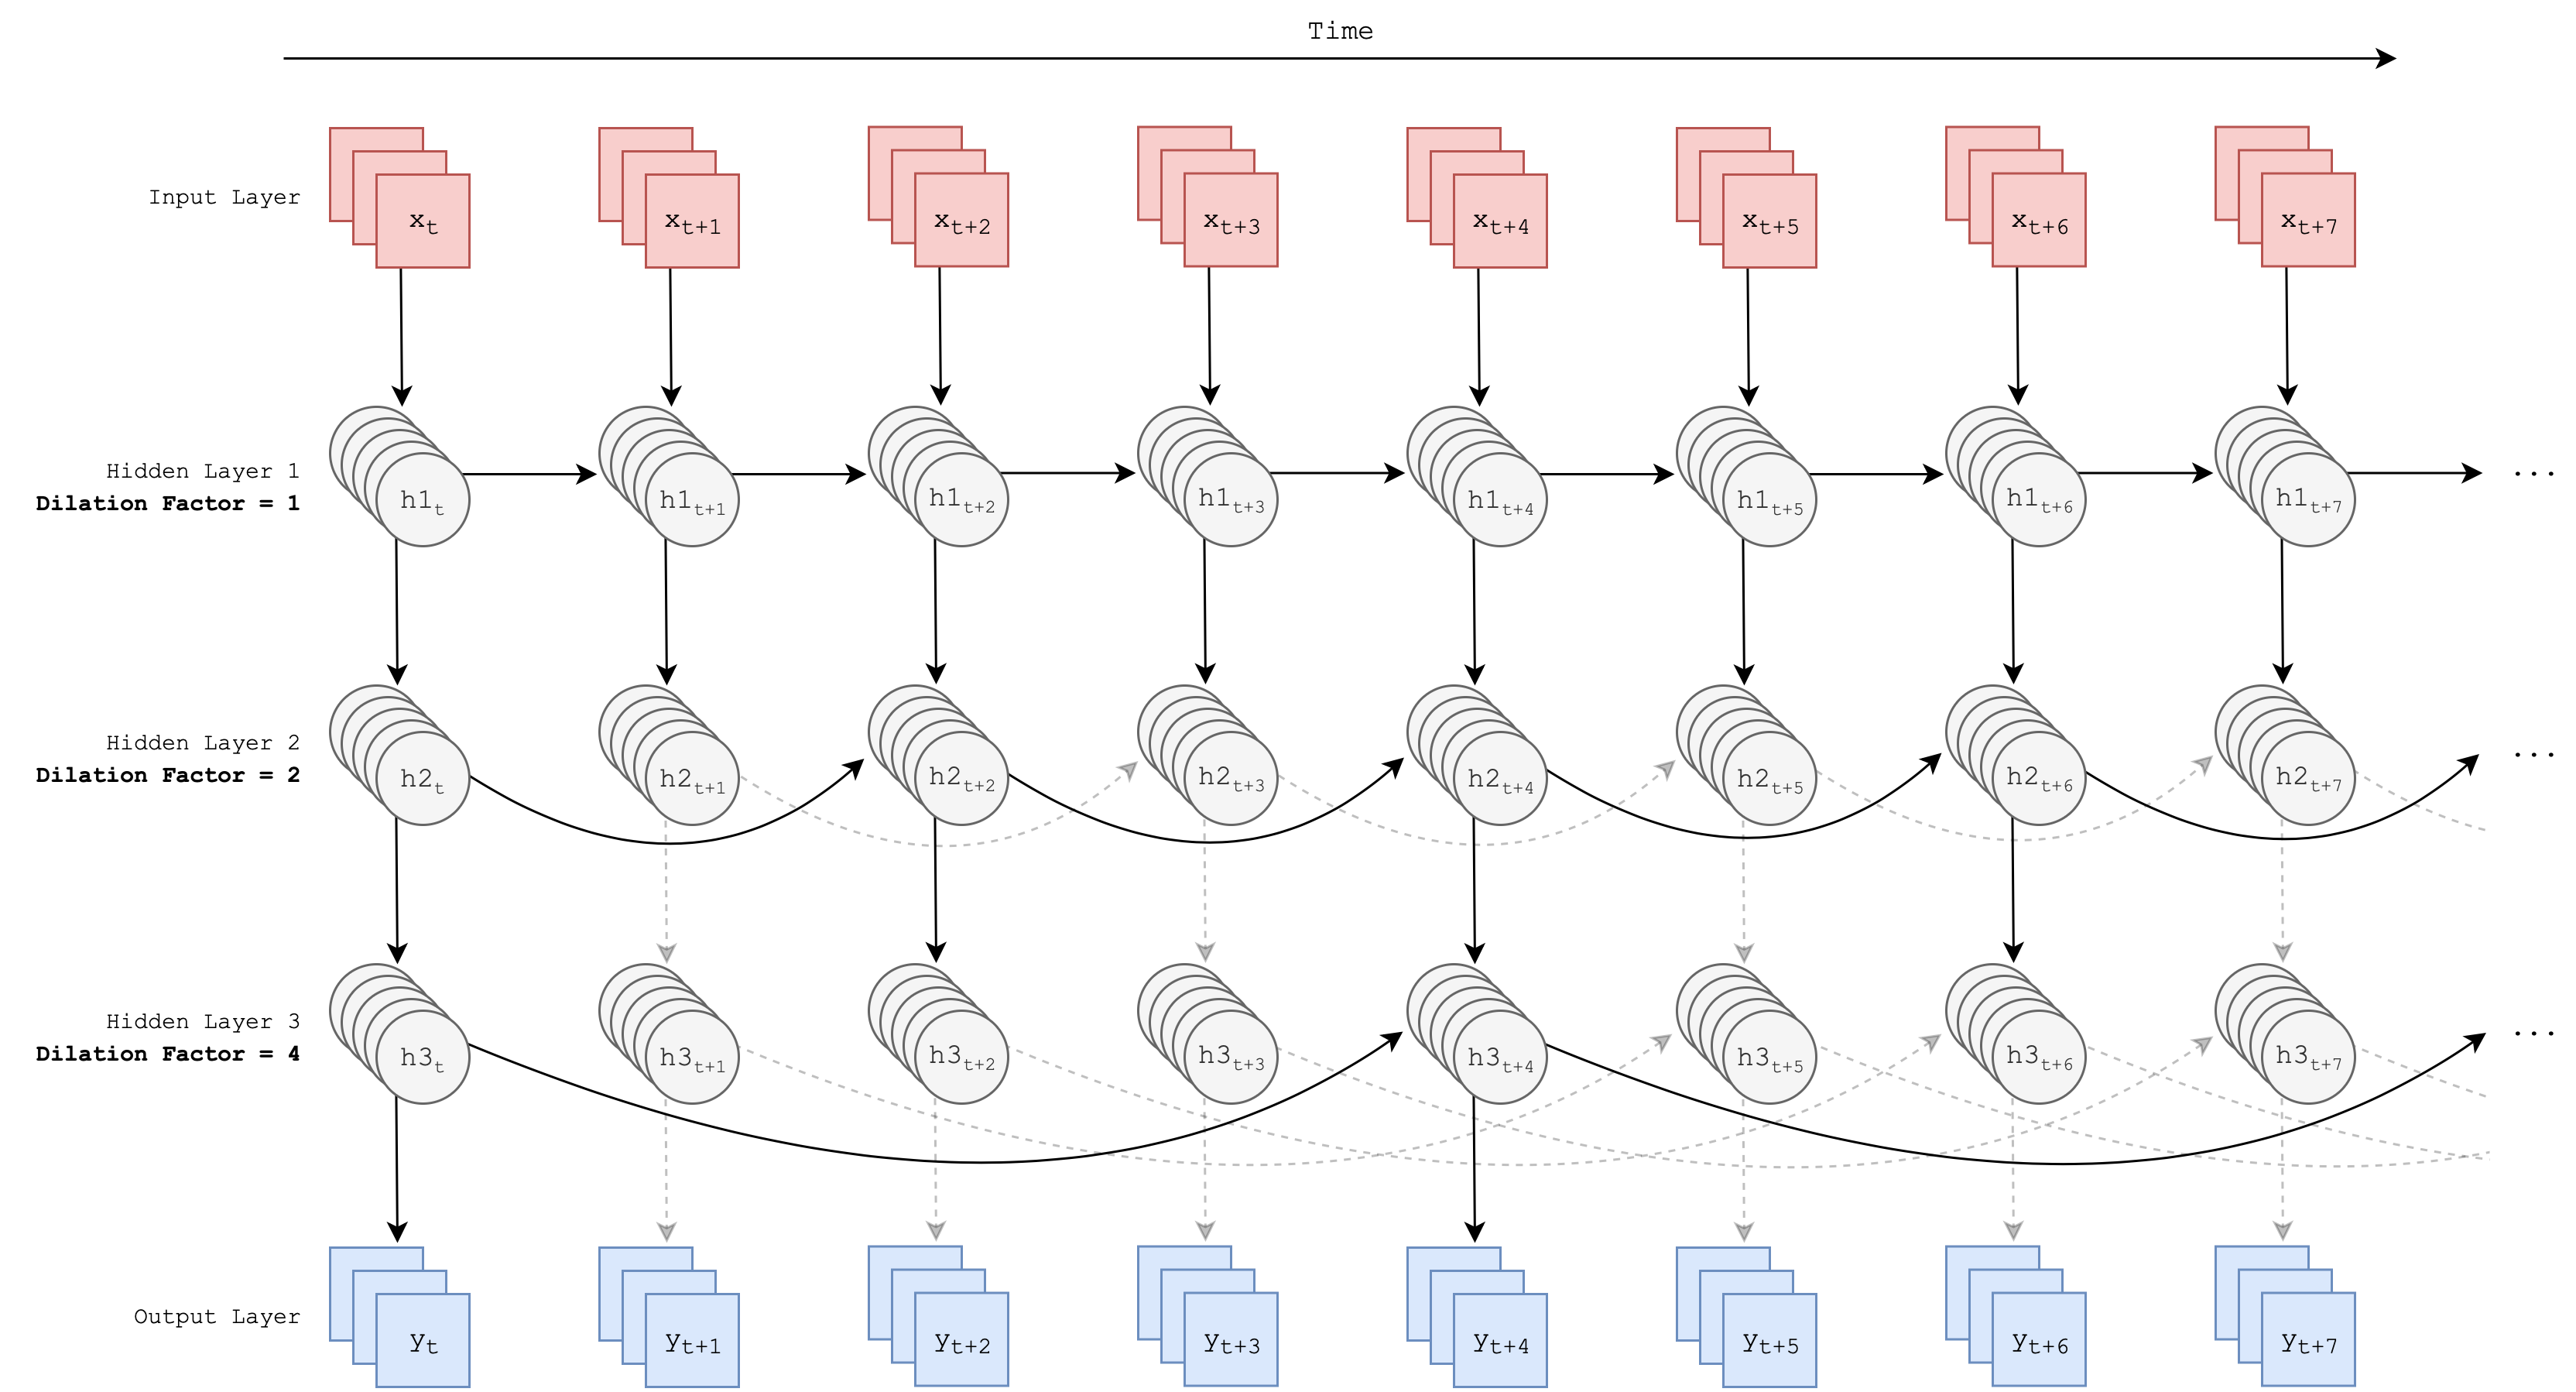
\includegraphics[width=1\textwidth,height=\textheight]{Images/dilatedrnn.png}
\caption{An example of a three-layer dilated RNN with dilation factors
1, 2, and 4.}
\end{figure}

As well as the multiplicative nature of long-term musical structure,
compositional conventions also define notes relative to each other in
the multiplicative domain in that different note lengths are all half or
double of some other note length (e.g.~a semi-quaver occurs twice as
often as a quaver; a quaver occurs twice as often as a crotchet and so
on). The parallels between this temporal structure intrinsic to musical
composition and a dilated RNN's structure are clear:

\begin{figure}
\centering
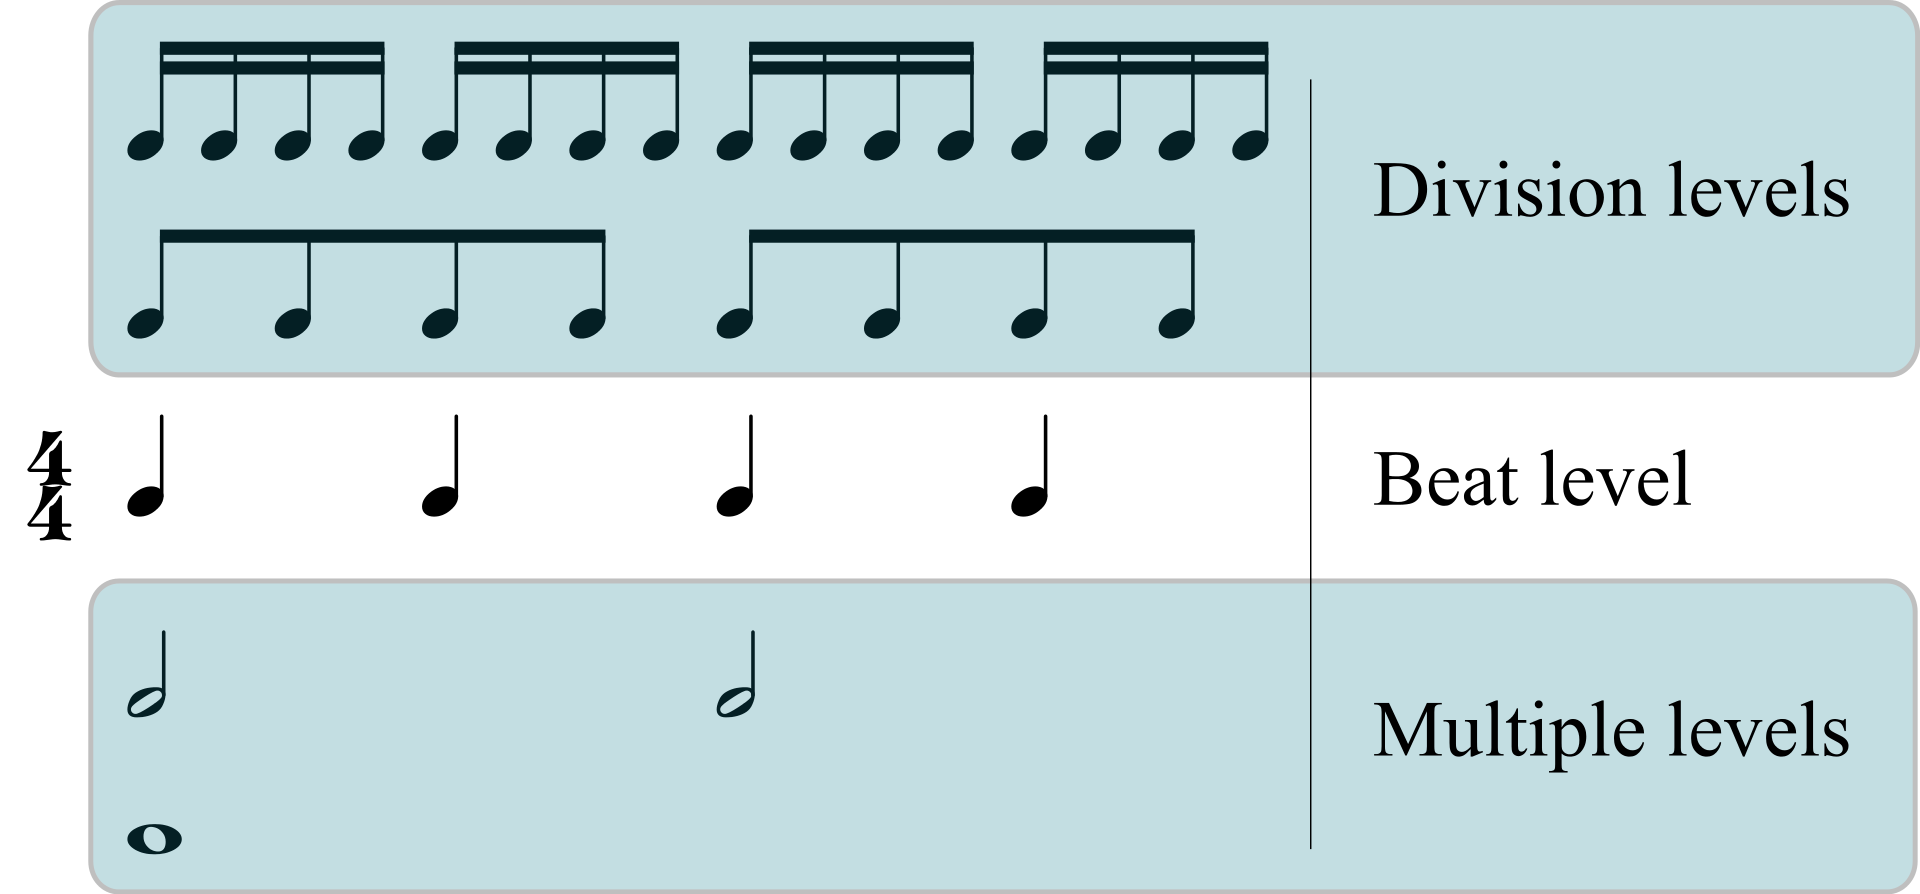
\includegraphics[width=0.7\textwidth,height=\textheight]{Images/Metric_levels.png}
\caption{Structural multiplicative hierarchy found within musical
scoring conventions; notes are all multiplications of each other in the
domain of doubling / halving.}
\end{figure}

Mathematically, dilation can be achieved by simply reconnecting the
network's layers such that all of the aforementioned recurrent
operations are done with respect to \(t-D_l\) rather than \(t-1\) where
\(D_l\) is the dilation factor of layer \(l\). Enhanced parallelisation
can be achieved by computing dilated layers together at the same time as
illustrated below:

\begin{figure}
\centering
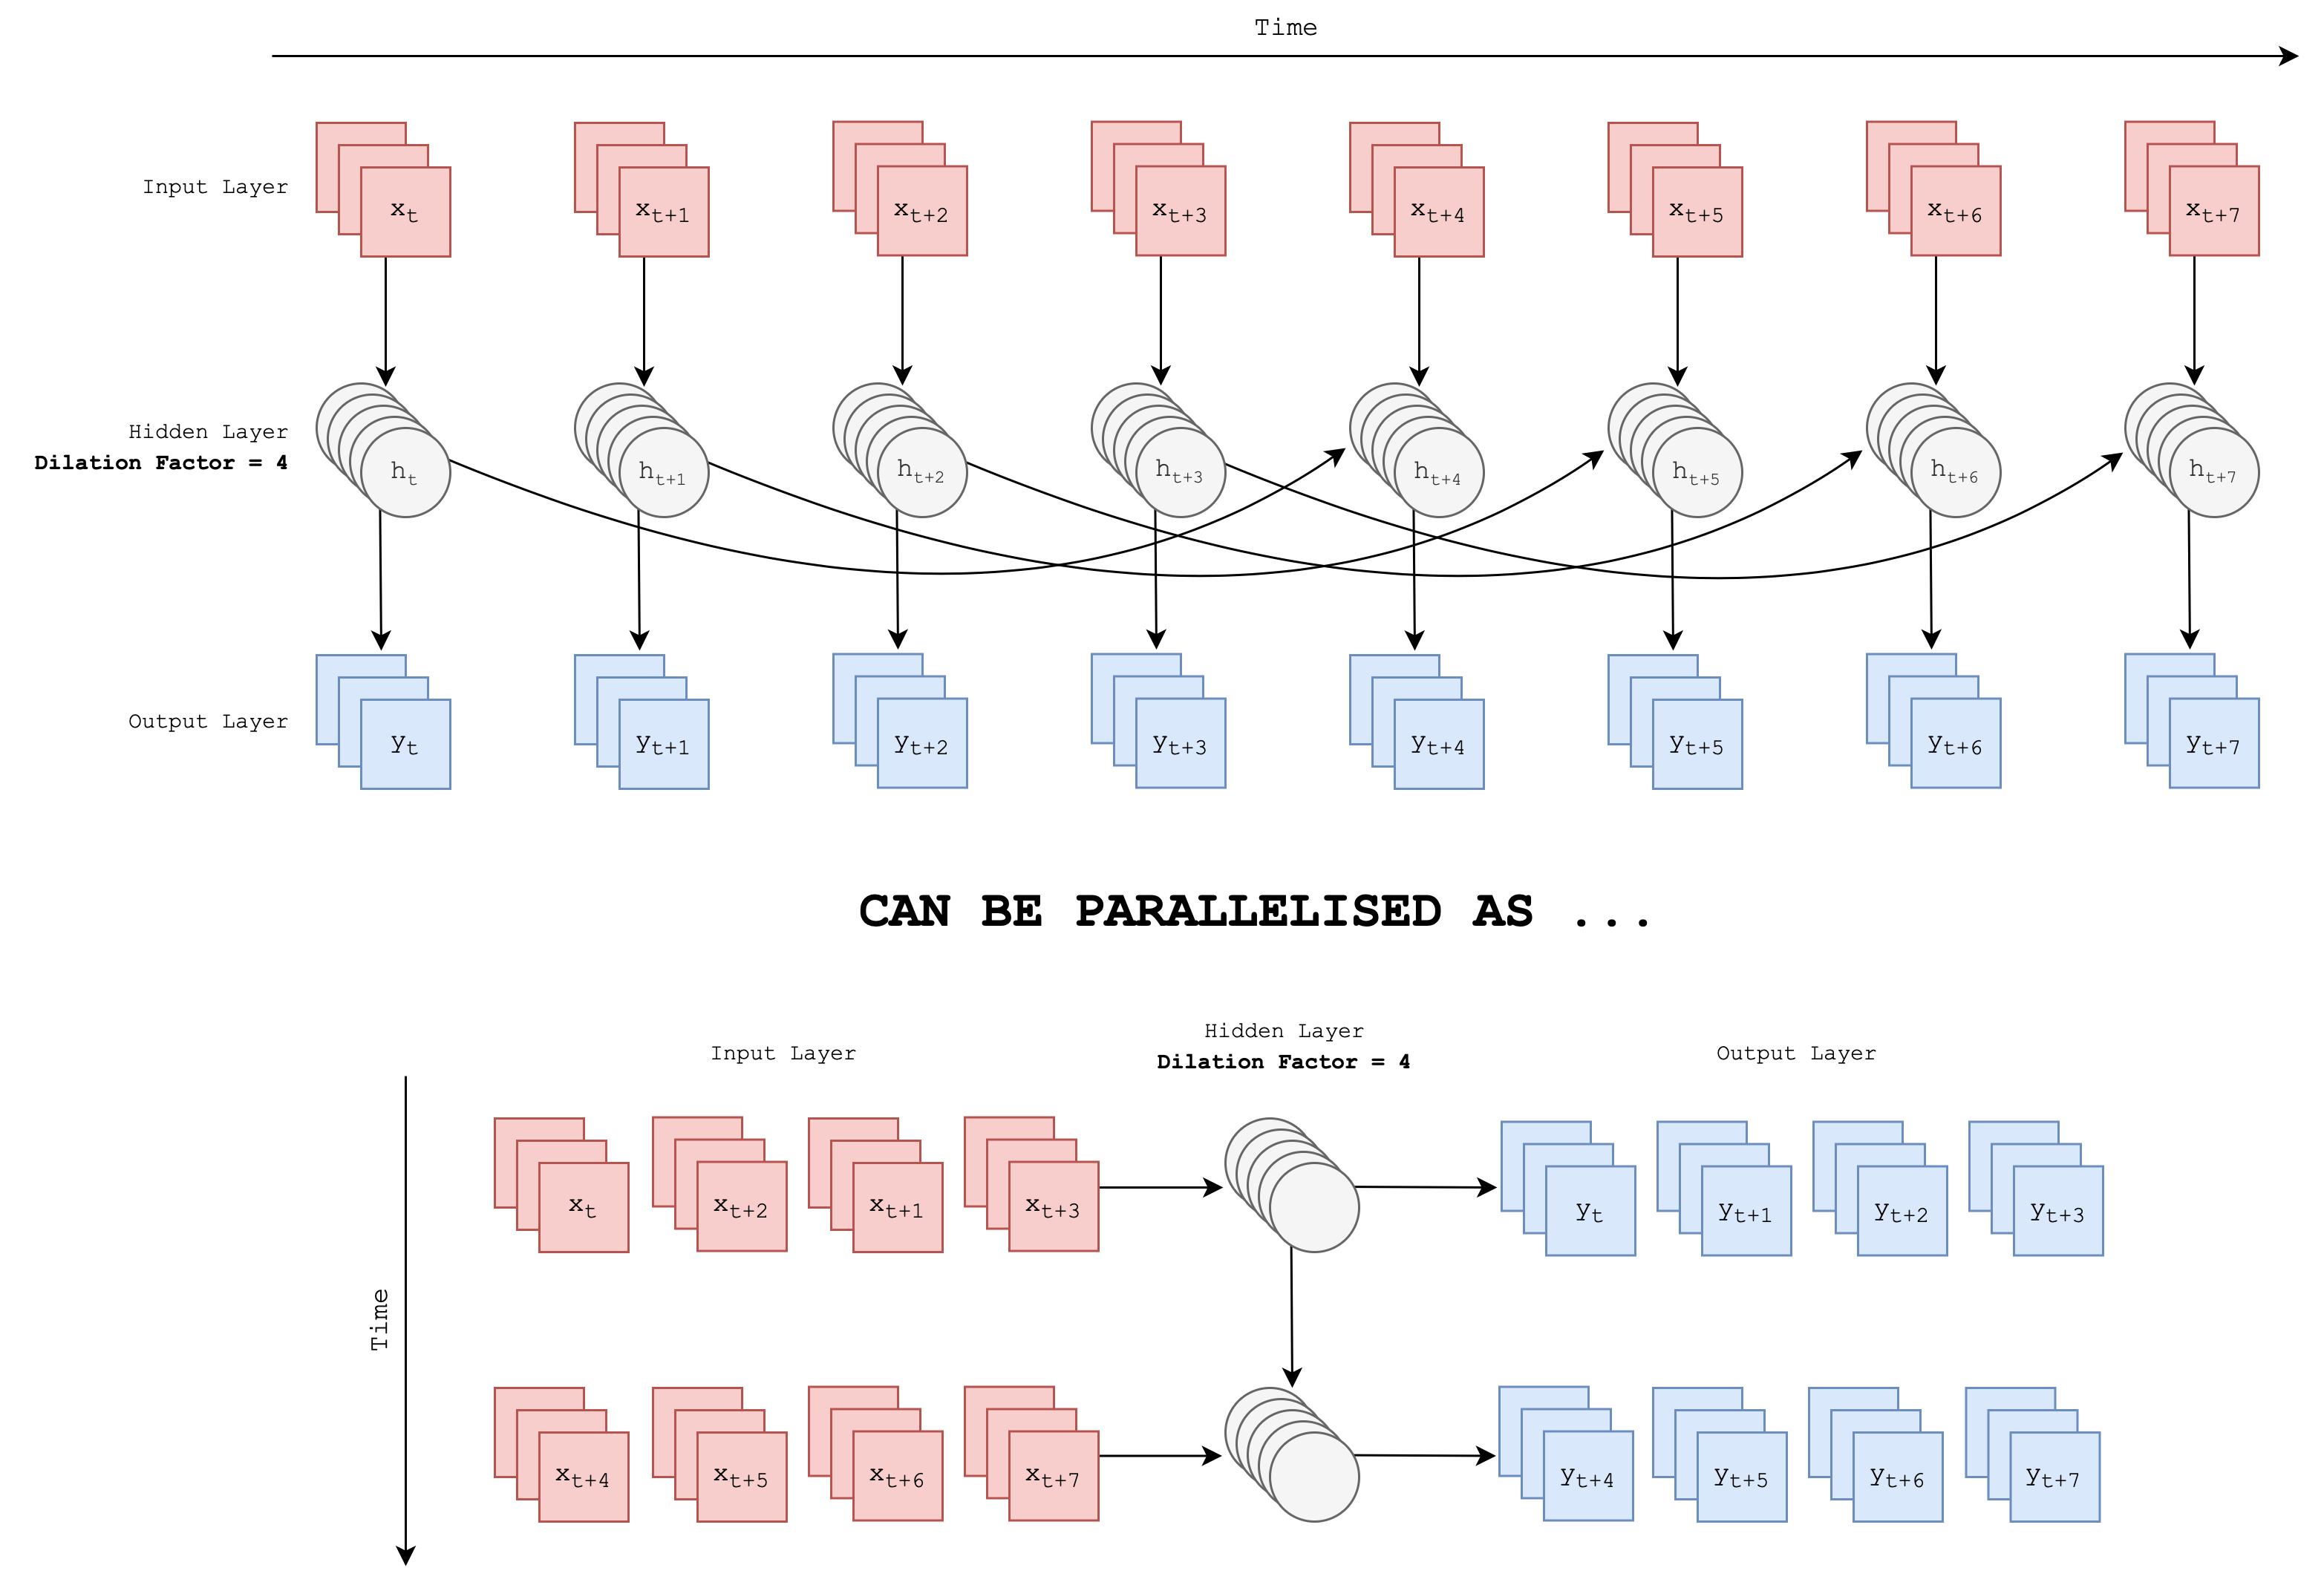
\includegraphics{Images/dilatedrnnparallel.png}
\caption{Diagram illustrating the parallelisation opportunities offered
by dilation in recurrent neural networks.}
\end{figure}

The four chains of recurrent units shown at the top of this diagram can
be computed in parallel rather than at separate time steps as all of
them occur across the same \emph{distance} in time. This can have huge
performance implications where parallel computation is enabled such as
when utilising GPUs to train a model. Inputs and connection weights may
simply be concatenated and computed together rather than at separate
time steps.

\hypertarget{introducing-harmonic-invariance}{%
\subsection{Introducing Harmonic
Invariance}\label{introducing-harmonic-invariance}}

The consideration of musical theory is the main inspiration for the
following section. There is a large amount of documentation and research
surrounding musical theory which a reader could investigate should they
wish to supplement this paper with additional context. However, the
essentials and relevant points are included for convenience.

In general, compositions are written with respect to a \textbf{key}
which in part determines the scales upon which harmonics and chords for
a piece are constructed. Each key is simply a transformation or rather a
transposition of another through some number of shifts up or down.

\vspace{35px}

\begin{figure}
\centering
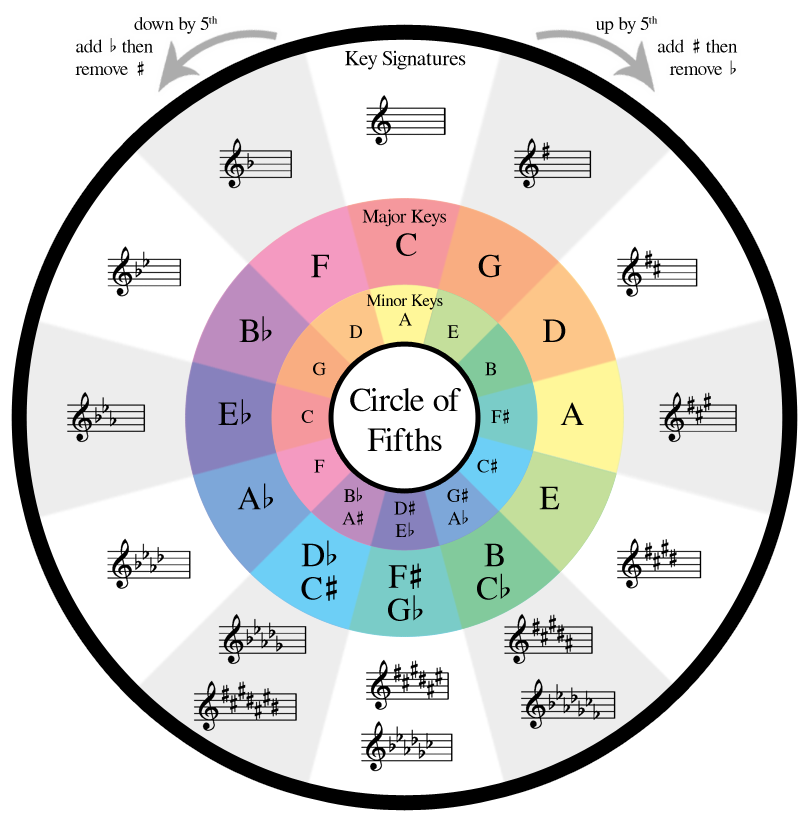
\includegraphics[width=\textwidth,height=0.4\textheight]{Images/flypaperfifths.png}
\caption{The Circle of Fifths. Note that increasing the root note by a
fifth (five notes) is equivalent to going down by four notes and vice
versa.
\newline\textit{Sourced from \href{https://flypaper.soundfly.com/write/how-the-circle-of-fifths-can-help-your-songwriting/}{Soundfly's FlyPaper}}}
\end{figure}

\begin{figure}
\centering
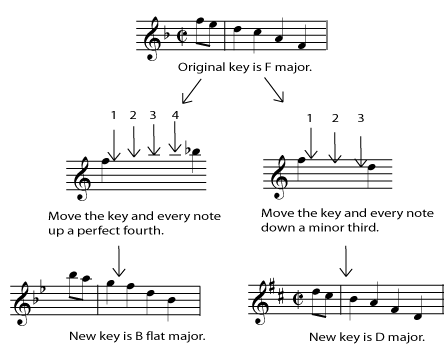
\includegraphics[width=\textwidth,height=0.3\textheight]{Images/transp3b.png}
\caption{Scored example of a transposition from F major to B flat major
and D major.
\newline\textit{Sourced from \href{https://www.earmaster.com/music-theory-online/ch06/chapter-6-4.html}{EarMaster}}}
\end{figure}

This highlights a potential issue with many pre-existing attempts at
composition using neural networks and the limitations of some
distribution estimators such as Restricted Boltzmann Machines
{[}\protect\hyperlink{ref-sutskever2009recurrent}{65}{]} and Neural
Autoregressive Distribution Estimators
{[}\protect\hyperlink{ref-uria2016neural}{66}{]}. Many modern approaches
utilise these units in their models, which involve a fixed distribution
generating probabilities for each note deterministically, i.e.~one
probability for each possible note. Whilst this may seem initially ideal
for modelling the played notes on a piano statistically, these
approaches constrict calculated probabilities to fixed note positions on
a piano rather than note positions relative to other notes at a given
time state.

All of the harmonics present in music (aside from some intentional
dissonances) are entirely relative by nature. For example, if we
represent all playable MIDI notes as a 128-element binary vector with a
value of 1 representing a played note and 0 otherwise, a major triad
chord can be represented as:

\[... 0100010010 ...\]

This arrangement forms a major triad with respect to some root note /
key regardless of its absolute position in the input sequence; the only
rule for creating a major triad is to start with a note, then add its
major third (always 4 keys to the right of the root) and perfect fifth
(always a further three keys from the major third). This highlights the
property of \textbf{harmonic invariance} in music. Many of the
aforementioned solutions including most of the ones discussed in the
section on \protect\hyperlink{competitiveexistingsolutions}{pre-eminent
solutions} utilise architectures which mean that they would have to
learn each transposed chord separately. This approach immediately
ignores this concept of harmonic invariance and relativity in musical
scoring which is key to having a model understand its rules beyond a
single key.

Inspiration can be drawn once more from convolutional neural networks
which achieve invariance in analysing images by utilising multiple
kernel functions which each learn relative localised features in the
data as they are passed over an image. To achieve this, the input data
is cross-correlated meaning that the output is identical for any set of
inputs \((u_{(i + x)}, v_{(j+x)})\), for all fixed \(i,j\) and any
offset \(x\).

The idea is to apply this concept to the model's architecture such that
all inputs of the same offset are treated equally to each other, by
considering their positions relatively rather than absolutely.

\hypertarget{the-finalised-model-architecture}{%
\subsection{The Finalised Model
Architecture}\label{the-finalised-model-architecture}}

The culmination of the above sections results in a network consisting of
dilated GRU or LSTM units, tied such that they are invariant temporally
and harmonically by keeping some recurrent connections between time and
others between the harmonics of an input. Both GRU and LSTM units were
trialled and evaluated due to their similarities and applicability to
the task. It was important to be mindful of the project's objectives
when considering the use of the above features. There was no intention
to try and pre-train the model or constrain it by imposing
considerations of musical theory (as the assumptions these
considerations incorporate could be less applicable to a mathematical
model than they are to humans); dilation and other concepts were applied
in order to augment a network's ability to consider multiple temporal
dimensions and mitigate the previously-mentioned issues with RNNs, but
also have the advantage of appearing intuitive in the domain of musical
composition.

Four hidden layers were used with exponentially increasing dilation
factors ranging from 1 to 8 as has been proved to be the most effective
arrangement computationally
{[}\protect\hyperlink{ref-chang2017dilated}{64}{]} and is also the most
logical arrangement for capturing the different temporal resolutions in
music. Two configurations for the hidden layer sizes were attempted:

\begin{enumerate}
\def\labelenumi{\arabic{enumi}.}
\tightlist
\item
  The first hidden layer was given 1536 units; each layer following this
  was given half as many units as its predecessor down to the output
  dimension of 192.
\item
  All hidden layers were given 768 units, 4 times as many as the input
  dimension.
\end{enumerate}

There is no agreed upon rule or practice for hidden layer configuration,
but common approaches are to attempt layer sizes in an inverted
pyramidal configuration like that described in (1.) or for all layers to
have a similar number of units as in (2.)
{[}\protect\hyperlink{ref-doi10108001431160802549278}{67}{]}. Most
existing solutions maintain a consistent number of units in each layer.
In order to arrive at these numbers some preliminary testing was carried
out to compliment the knowledge and intuition already gained from
previous work; it was found that networks with fewer nodes sometimes
struggled to learn effectively whilst increasing the nodes beyond these
figures massively increased computational cost and seemed to increase
the likelihood of overfitting. The exponentially increasing dilation
factor layer-by-layer does reduce the overall number of recurrent
calculations done at each step as was noted in the
\protect\hyperlink{dilation}{relevant section} which helps alleviate the
issues mentioned earlier regarding vanishing and exploding gradients.

The hidden layers themselves were comprised of either GRU or LSTM units
and wrapped with dilation (the implementation of dilation is clear from
the code included with this report, roughly it involves transforming the
inputs to spread appropriately across the different layers and imposing
skip connections at certain time steps). Surrounding these layers is a
linear distribution of the mood at the point of input to the main graph;
at the end a linear output layer is appended to ensure something of the
correct dimension is outputted regardless of the hidden layer
configuration above. The dimension of the output \(D_{\text{output}}\)
is equal to \(D_{\text{input}}\) so that it can be converted back to
MIDI if required; clearly the outputs represent the models' choices in
playing notes and the associated times and velocities to go with these
choices.

\hypertarget{training}{%
\subsubsection{Training}\label{training}}

In order to train the models, it was necessary to utilise
backpropagation through time
{[}\protect\hyperlink{ref-werbos1990backpropagation}{52}{]}; it is
during this process that dilation becomes invaluable through minimising
the total number of connections in paths between nodes at different
times which has a positive computational impact for the execution of the
BPTT algorithm as well as further mitigating vanishing and exploding
gradients. This also contributes to improving the model's ability to
extract long-term dependencies.

Cross entropy loss was decided upon to quantitatively measure the
models' performance in the compositional task. A lower value of this
performance metric implies lower entropy in a model's generated outputs
/ note probability predictions which is equivalent to saying these
outputs are similar to the training inputs. Note that using cross
entropy loss is equivalent in implementation to the negative
log-likelihood loss function applied after a softmax calculation layer
in a network. This is a fact we rely upon in the quantitative evaluation
further on in the report.

This loss criterion expects an input tensor containing probabilities
associated with each of \(D_{\text{output}} = 192\) classes
corresponding to the possible values discussed as part of the
representation, such an output is returned for every element of every
training sequence of each batch. The criterion input's dimensions are
therefore:
\[\text{Batch Size} \times \text{Training Sequence Length} \times D_{\text{output}}\]

A \emph{target} is also passed to the criterion which contains the
corresponding ground-truth class indices, the target is essentially the
input before it is one hot encoded but also shifted forward in time by
one step. This is of dimension:
\[\text{Batch Size} \times \text{Training Sequence Length}\]

Then for every element of every training sequence, the following
formulation of cross entropy is applied where \(x\) is a \textbf{single
time step's outputted vector of probabilities} associated with each of
the \(D_{\text{output}}\) classes and ``class'' corresponds to the
\textbf{target's ground-truth class index}:

\[
\operatorname{loss}(x, \text {class})=-\log \left(\frac{\exp (x[\text{class}])}{\sum_{j} \exp (x[j])}\right)=-x[\text {class}]+\log \left(\sum_{j} \exp (x[j])\right)
\]

Training was carried out with a 20:60:20 test:train:validation split
applied to the MAESTRO and author-created ambient datasets with 250
training batches per epoch and 75 validation batches (batch size was set
to 32). Multiple optimisers were trialled after applying BPTT; Adam
{[}\protect\hyperlink{ref-kingma2014adam}{68}{]} was found to be the
most succesful which is a recent and popular gradient descent algorithm.
The models were then tested on the unseen test data; the resulting
figures for each model's loss are included in the tables following this
section.

The training curves for each configuration on the MAESTRO dataset are
shown below:

\begin{figure}
\centering
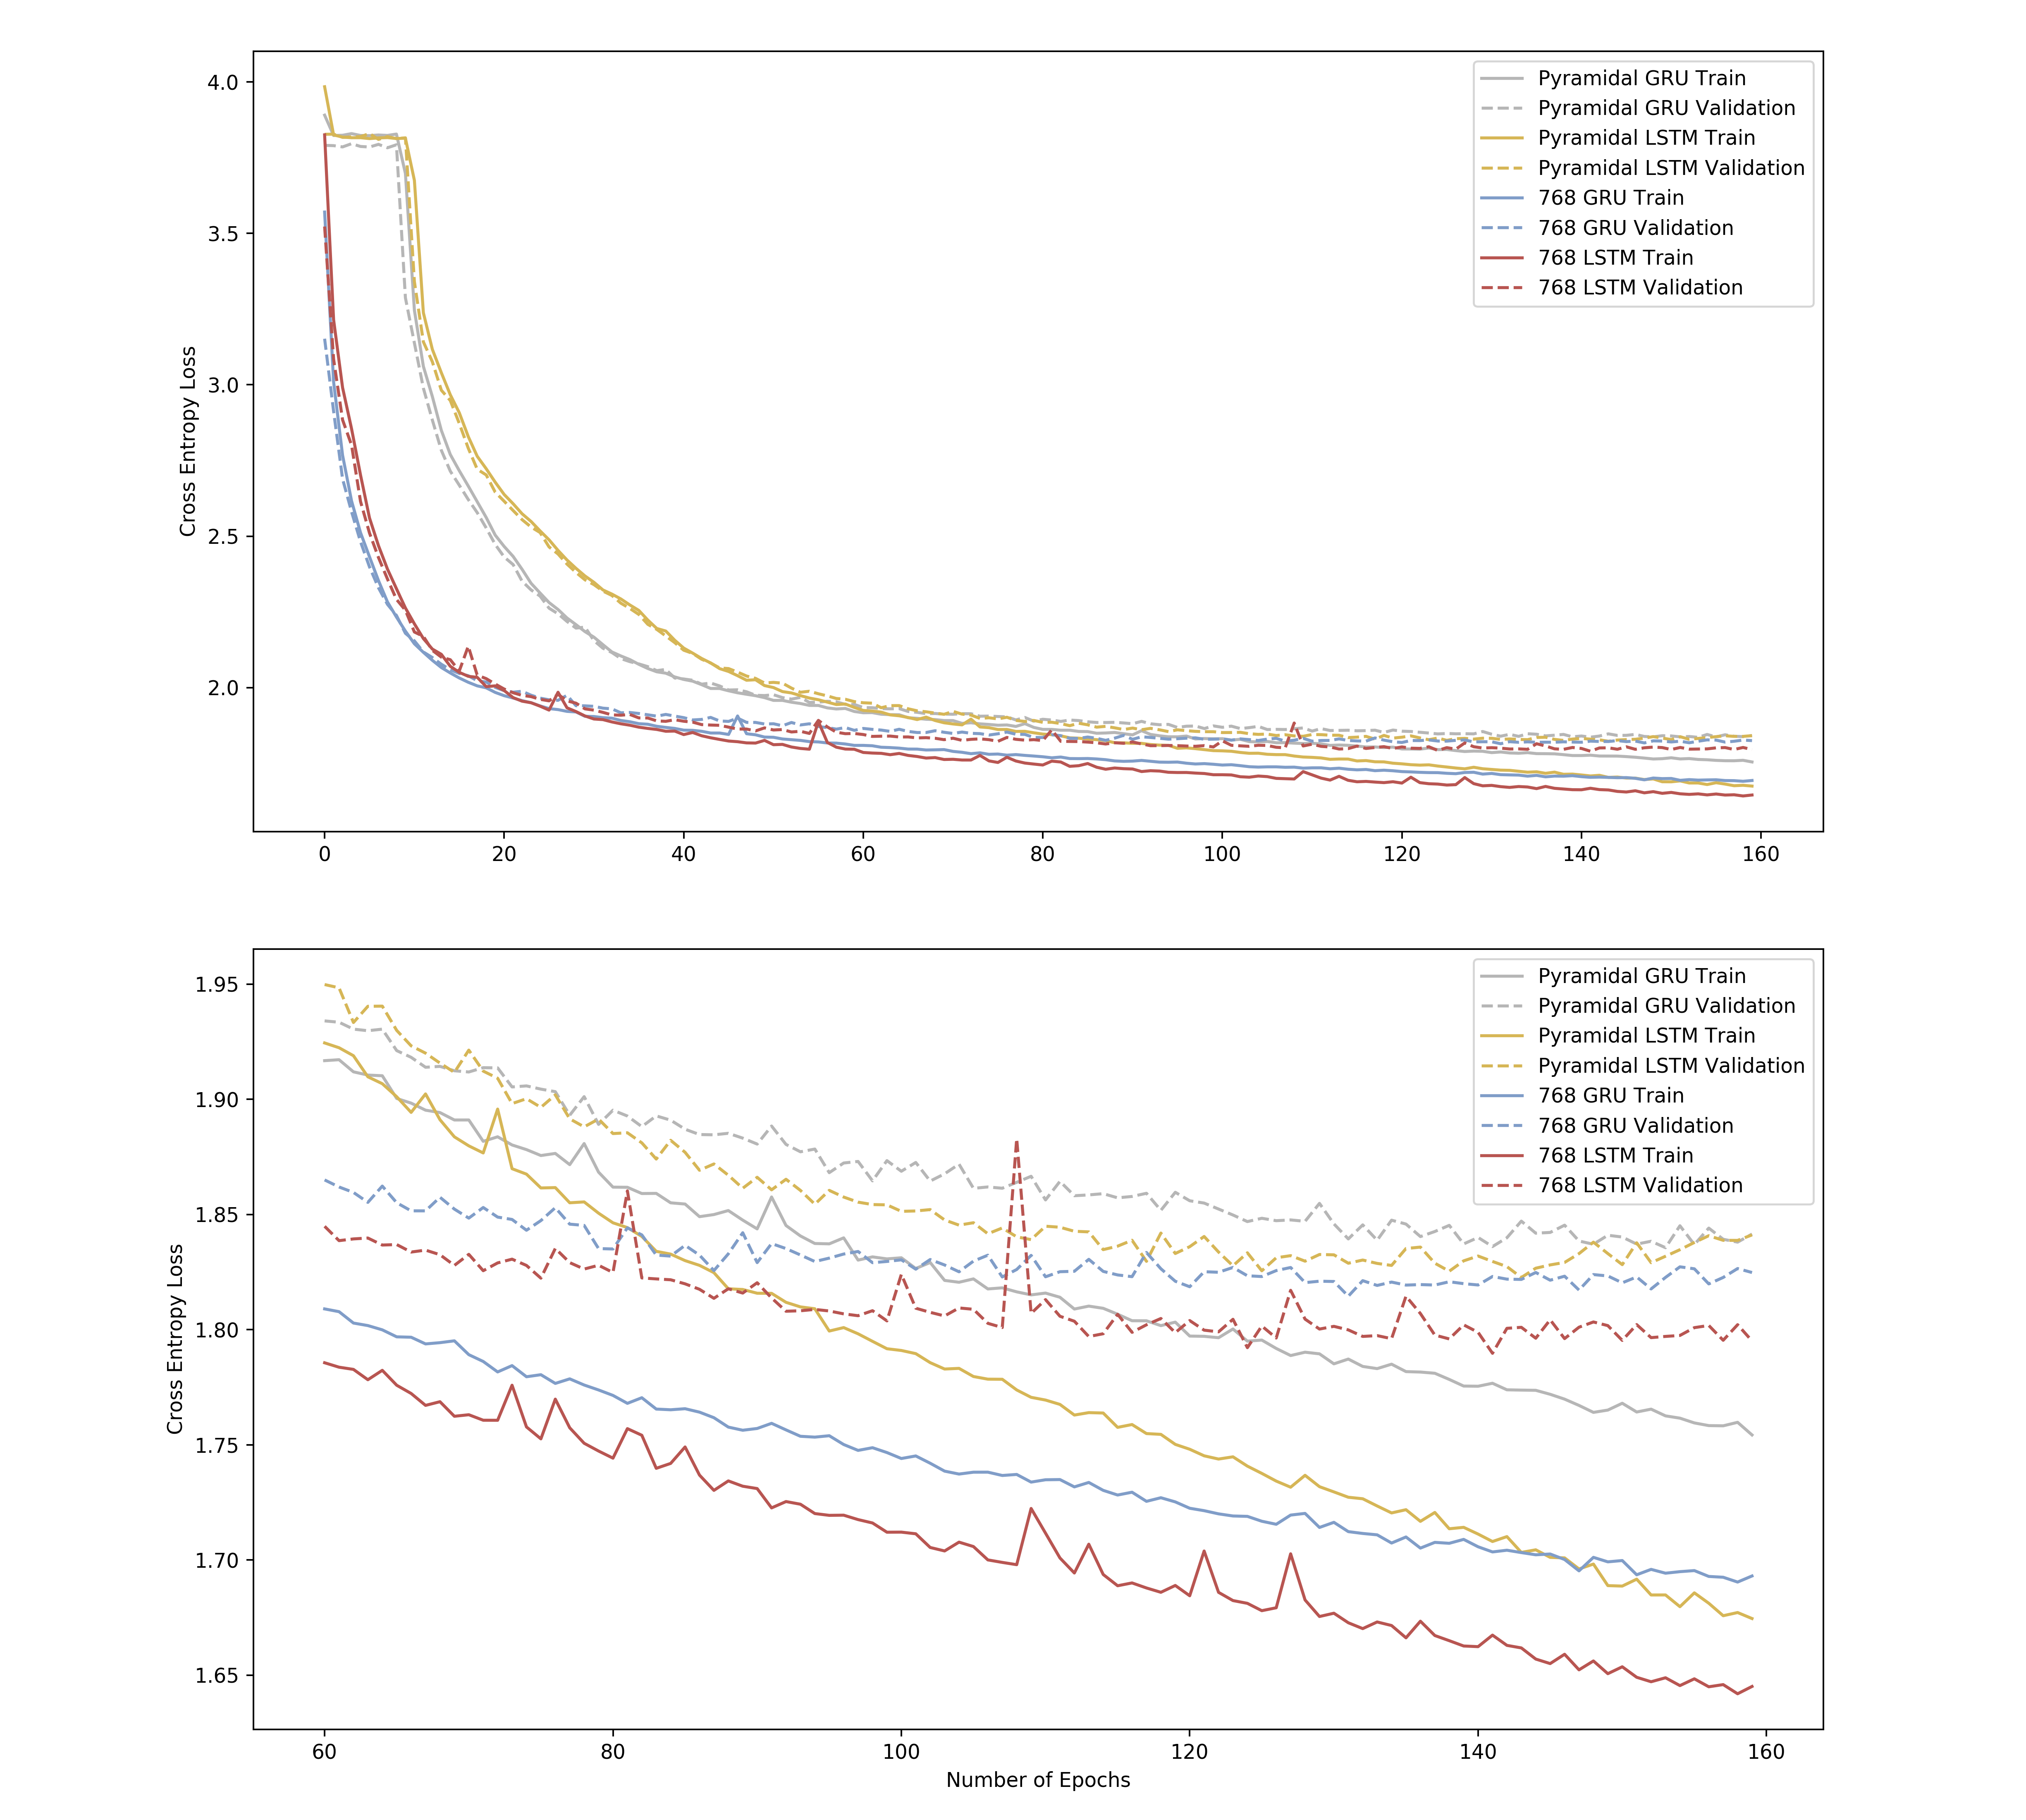
\includegraphics{Images/loss.png}
\caption{Cross entropy loss plotted against number of epochs for each
model architecture, the top graph includes a full 160 epoch curve whilst
the bottom omits the first 60 in order to give a better view of eventual
loss values and convergences in validation loss.}
\end{figure}

From this it can be seen that the model utilising LSTMs in the
non-pyramidal configuration worked best; this model along with the
GRU-based model in an identical configuration were selected for further
comparisons with other research. The pyramidal model exhibited strange
behaviour in initially plateauing and it was more prone to overfitting
as can be seen by the greater divergence in training and validation
losses throughout training.

The models were trained using compute resources provided by the
University of Warwick
{[}\protect\hyperlink{ref-warwickcomputenodes}{43}{]}, namely a server
with a GTX 1050Ti graphics card, 64GB of RAM and an Intel i5-7500
processing unit. Most of the referenced papers had training environments
of at least equivalent computational effectiveness and were usually
significantly better equipped. Bearing this in mind it is relatively
clear to see that dilation and the use of GRUs especially leads to an
exceedingly computationally efficient model. Some papers cite training
times spanning days or even weeks before reasonable convergence and
outputs are achieved whereas the architectures described in this project
reach usable states of near-minimal loss in around 24 hours.

\setlength\extrarowheight{1pt}
\begin{table}[H]
\centering
\caption{The time in minutes taken per epoch during training of different model architectures.}
\vspace{1em}
\begin{tabular}{llcc} 
\toprule
                             &                                    & \multicolumn{2}{c}{\textbf{Recurrent Unit Type}}  \\
\textbf{Dilation}            & \textbf{Hidden Unit Configuration} & GRU   & LSTM                                      \\ 
\hline
\multirow{2}{*}{Dilated}     & All 768                            & 8:24  & 9:58                                      \\ 
                             & 1536, 768, 384, 192                & 8:52  & 10:46                                     \\ 
\multirow{2}{*}{Not Dilated} & All 768                            & 9:05  & 10:45                                     \\ 
                             & 1536, 768, 384, 192                & 9:40  & 11:39                                     \\
\bottomrule
\end{tabular}
\end{table}

Of course, these times are relative to the system upon which the network
is trained. However, they are included here for illustrative purposes of
the relative differences between the different configurations. It is
impressive to consider that not only do dilated networks train faster,
they also reach lower loss values in a lower number of epochs implying
they are superior in every measurable respect.

It is proposed that with a training setup utilising a more powerful GPU
or arrays of GPUs the parallelisation opportunities dilation offers
would be further magnified and have a greater impact on the difference
in training times. The benefits of dilation are already impressive when
considered relative to the loss convergence and value after 160 epochs.

\hypertarget{generation}{%
\subsubsection{Generation}\label{generation}}

After training, it is relatively simple to generate pieces using the
models. The network parameter weights are saved to a file where they can
be recalled along with the initialisation of some starting values to
recurrently make predictions based on these learned parameters and
output these predictions in sequence to a MIDI file. The user is
prompted to provide sentimental input in the form of a six-element
vector similar to the ones associated with the training data; it is also
possible to input an initial note state or network parameter values as
``inspiration'' for the model due to this method of generation through
the harnessing of its predictions.

At each time-step the model's predictions (a vector of probabilities)
are utilised to determine a note state (it selects states with high
probabilities to record as 1's in a \(D_{\text{output}}\)-dimensional
vector with the rest of the values set to 0) which is then used as input
for the next time-step. These states are eventually written to a MIDI
file using the same conversion process as is applied to the training
MIDI data but in reverse. Interestingly, pieces are composed quickly
enough to be produced and played in real time which offers potential
inspiration for a variety of real-world applications of these models and
techniques.

All of the above processes are summarised and simplified in the diagram
below in order to offer an overview of the different components present
in the overall system and how they interact.

\begin{figure}
\centering
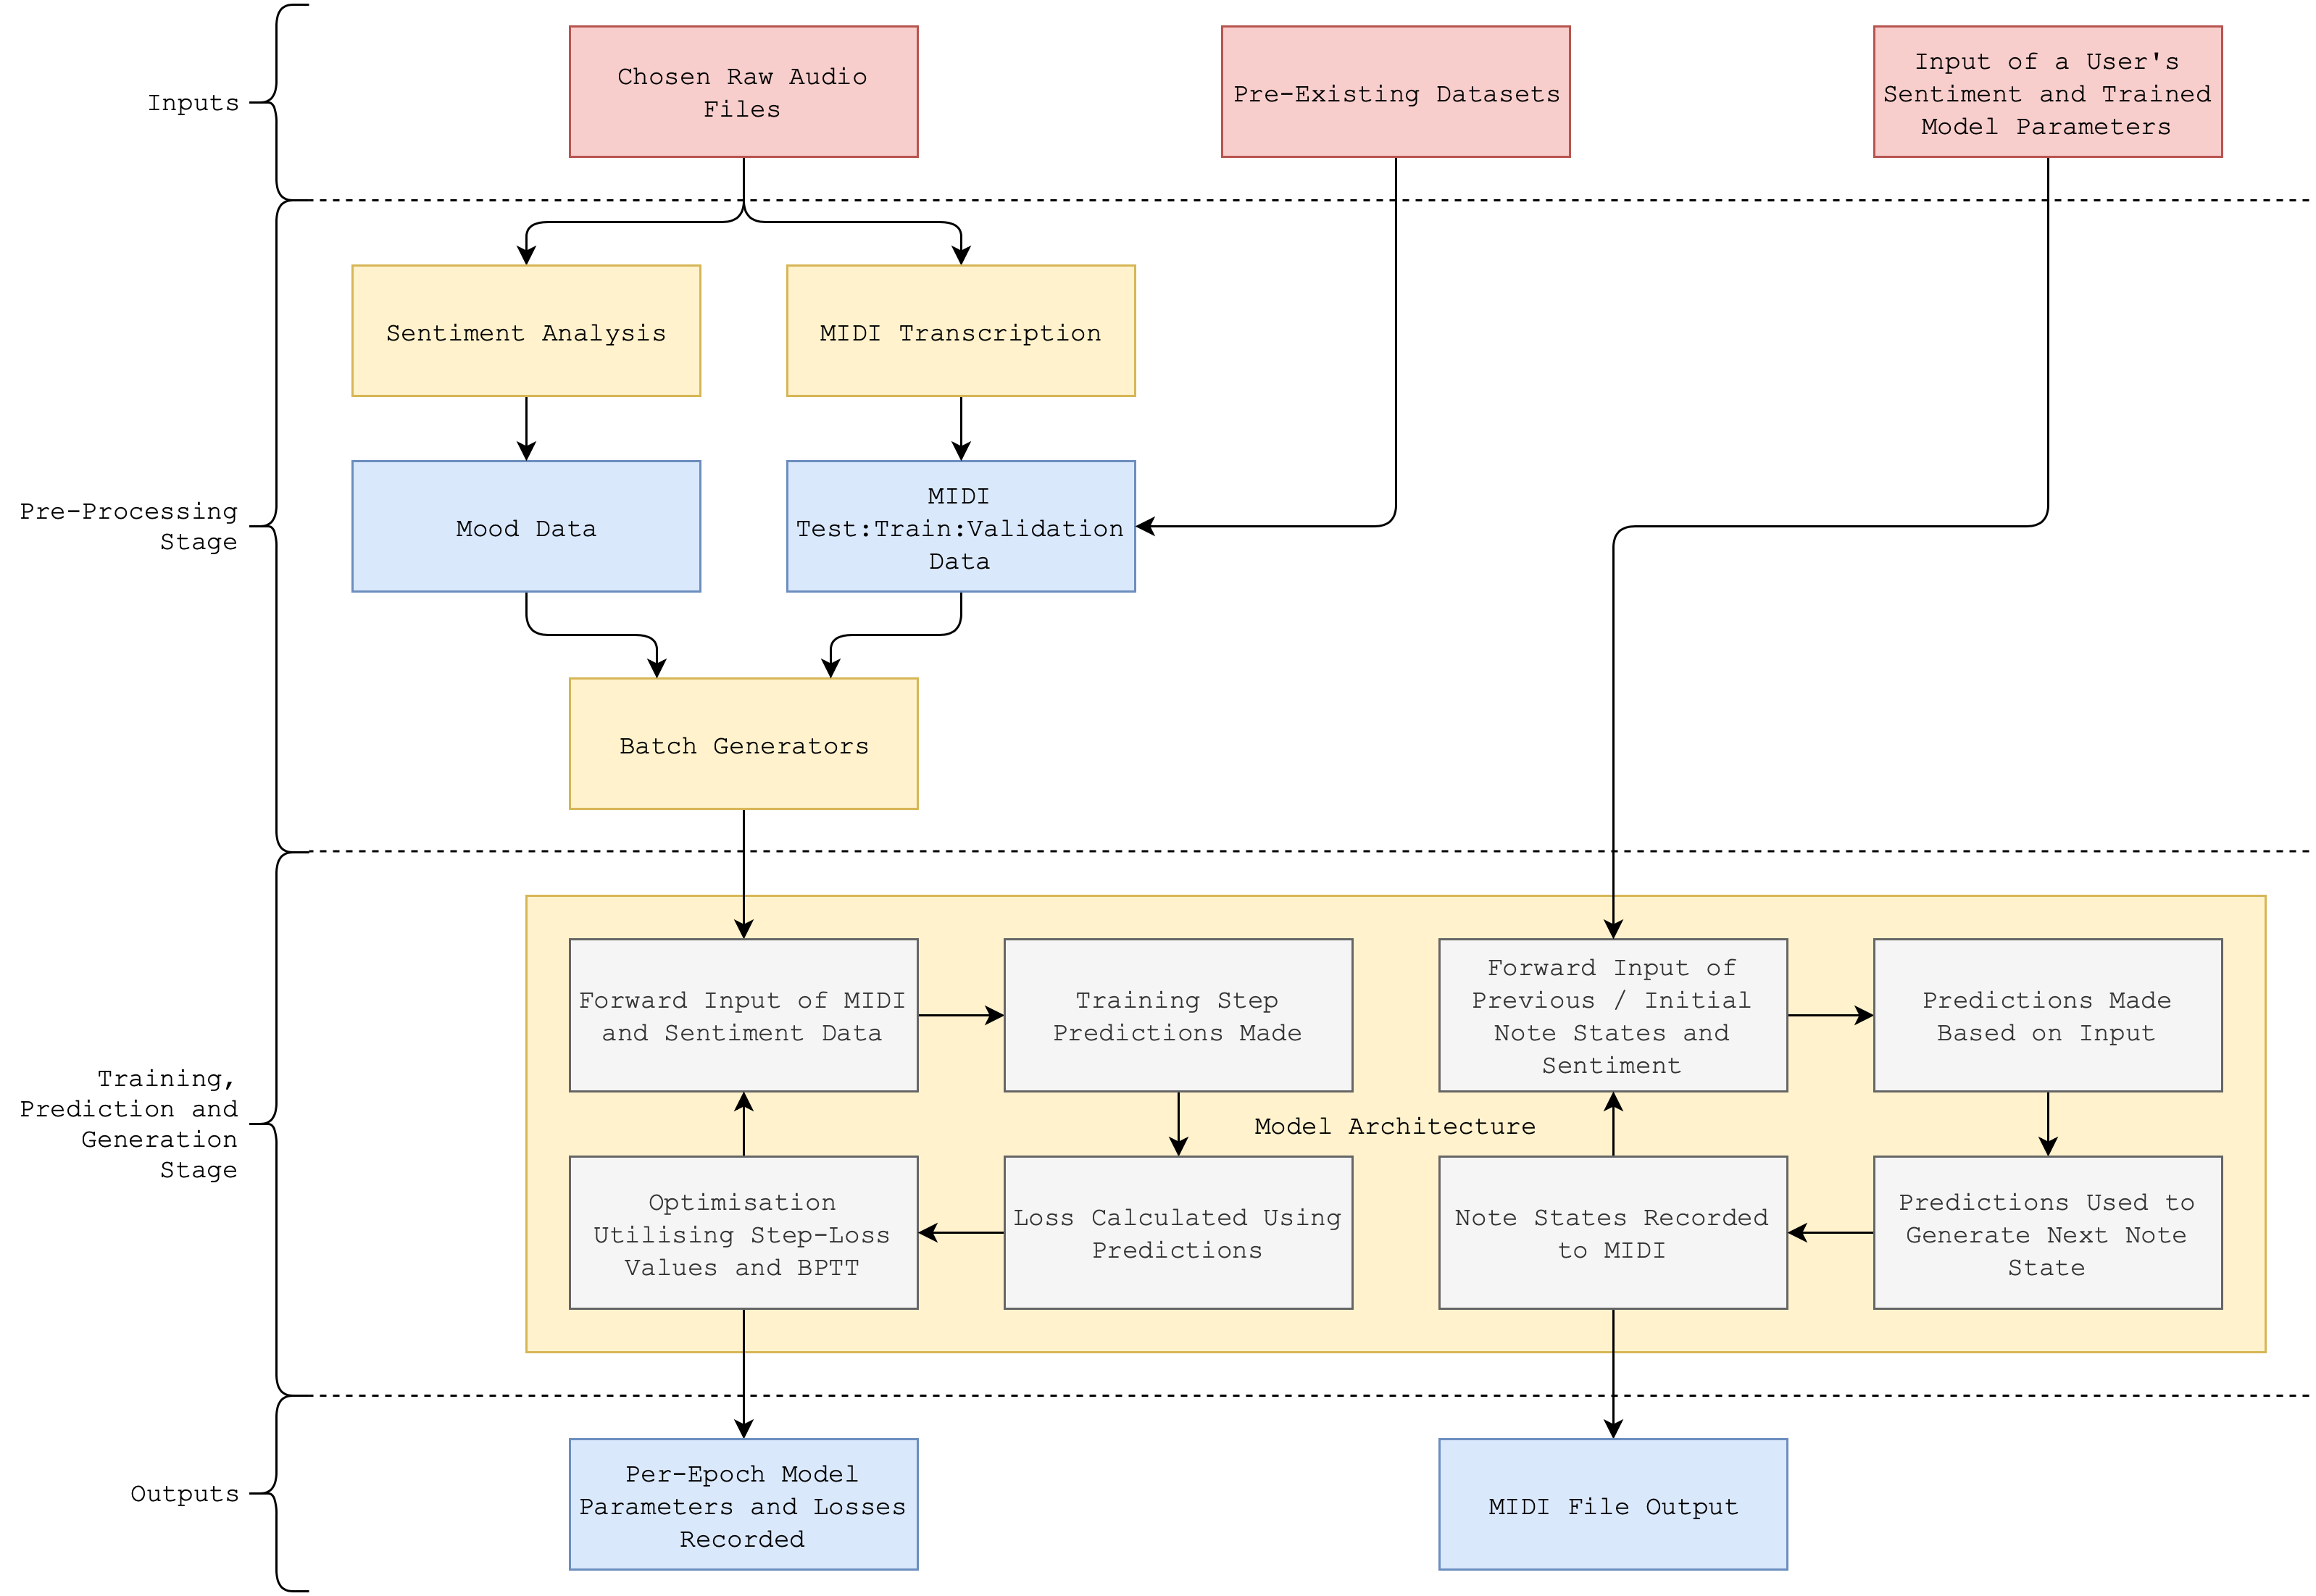
\includegraphics{Images/processdiagram.png}
\caption{Diagram illustrating the described data pipelines comprising
the processes of training and generating from one of the formulated
models.}
\end{figure}

\hypertarget{trialled-alternative-approaches}{%
\subsection{Trialled Alternative
Approaches}\label{trialled-alternative-approaches}}

Aside from the discussion in this section so far, some other approaches
were trialled mainly based upon hidden Markov models and fairly standard
LSTMs and RNNs. Data for the evaluation of these models is plentiful and
so is only quoted from pre-existing research in this report. The model
architectures described above surpass these more traditional and common
architectures in the majority of cases.

It was found that Markovian models fail to capture any complex long-term
dependencies and too closely represent interpolations of their training
inputs rather than learning any deeper structures within the data.
Previous work when compared to this work and a small number of models
comprising the current state-of-the-art are significantly worse in terms
of their output quality when assessed by humans and fail to capture more
complex features or represent dynamics effectively as is the case with
the models proposed here.

\hypertarget{testing}{%
\subsection{Testing}\label{testing}}

The modular nature of this project's implementation allowed for
individual testing to take place on each component. MIDI transcription
is an objective task such that the outputs validated the code, provided
they were accurate which indeed they were to within a small degree of
acceptable error. The model itself was validated and tested as has
already been discussed; its code was tested component by component
before being built into a system. Outputs were investigated and errors
appropriately dealt with during development in order to ensure the
system was carrying out its designated purpose effectively.

Sentiment analysis was comparatively much more subjective; though the
outputs of sentiment analysis could be tested to ensure that all of the
signal processing components and transforms were effective and correctly
mirrored the mathematics upon which they were based. Beyond this,
qualitative assessment and the use of human judgement was required in
order to ensure the mood characteristics that were captured seemed
relevant to the input pieces and that the outputs of the model were
coherent beyond loss metric values.

\hypertarget{evaluation}{%
\section{Evaluation}\label{evaluation}}

\hypertarget{internal-comparison-of-work}{%
\subsection{Internal Comparison of
Work}\label{internal-comparison-of-work}}

In addition to the training comparisons that have already been made, it
was necessary to evaluate the architectures described in terms of their
quantitative and qualitative performance. As was indicated by the loss
curves for the different models, it appeared that an architecture with
equal numbers of units in each of four layers performed best. It was
found that decreasing the number of layers or units much beyond this led
to less satisfactory results in terms of the complexity of the model's
outputs, especially when the generated compositions were assessed by a
human listener.

It could be said that the latter stages of a deep learning-based
development process often comprise this exercise of determining
parameters through experimentation; indeed the chosen combinations were
the result of optimisation over time and the consideration of fewer or
more layers and fewer or more units per layer. The final described
architectures are those deemed to strike a balance between being
sufficiently complex and not so complex that they suffer from serious
overfitting or complexity issues. It appeared that pyramidal
configurations with similar numbers of units to their equalised
counterparts had more of a tendency to suffer from validation and
training loss divergence meaning that the final `best' configurations
were deemed to be those with equal units across layers.

After training, it was important to assess the models using unseen test
data, as well as to perform qualitative assessment on their generated
compositions.

\begin{table}[H]
\centering
\caption{Average cross entropy loss for each trialled architecture when exposed to unseen test data from the MAESTRO dataset.}
\vspace{1em}
\begin{tabular}{llcc} 
\toprule
                             &                                    & \multicolumn{2}{c}{\textbf{Recurrent Unit Type}}  \\
\textbf{Dilation}            & \textbf{Hidden Unit Configuration} & GRU   & LSTM                                      \\ 
\hline
\multirow{2}{*}{Dilated}     & All 768                            & 1.84  & 1.82                                      \\ 
                             & 1536, 768, 384, 192                & 1.90  & 1.87                                     \\ 
\multirow{2}{*}{Not Dilated} & All 768                            & 2.22  & 2.09                                     \\ 
                             & 1536, 768, 384, 192                & 2.30  & 2.32                                     \\
\bottomrule
\end{tabular}
\end{table}

The outputs from the LSTM architectures seemed to be slightly more
structured in terms of the repetition of motifs and chords throughout
their generated pieces. This is likely due to their more powerful memory
cell representation allowing for the model to more easily replicate
long-term musical structure over time. When viewed in context of the
epoch length for each of the architectures, the slightly inferior GRU
compositions still appear potentially favourable if resource costs and
time are limited factors in the training phase. Again, it is clear that
dilation offers a vast improvement over previous work and likely goes
far in solving some of the key issues faced by recurrent neural
networks. This concept could potentially be applied to other problems
utilising RNNs with favourable results.

The two chosen architectures comprising of four 768 dilated GRU / LSTM
unit layers will be referred to as RDGRU and RDLSTM in further
evaluation sections (R meaning relativistic to indicate the harmonic
invariance achieved, and D indicating the dilation applied to the
recurrent units). The outputs of these architectures were utilised in
the survey to be discussed in the next section as well as being the
subject of a great deal of reflection by the author as many samples were
listened to and compared.

This stage was an important part of the evaluation as it is debatable
whether considering a model's propensity to accurately predict the
coming notes in a sequence actually determines how ``good'' the model
is. Again, this is an issue mainly borne of the nature of the task and
the subjectivity of music; it is fairly reasonable to consider that a
validated / tested model which does not overfit but produces a low loss
metric value in the prediction task must have a better grasp of musical
composition than one with a higher loss value as it is safe to assume
that the majority of mistakes must come from irregular timings and
out-of-tune note selections. It is likely that a model that plays in a
similar way to its training inputs must be closer to the goals of the
project than one that does not.

Another means of assessing the quality of the created architectures was
to generate a large number of pieces across the spectrum of mood and
compare their note distributions to that of the training data. Again, it
would be assumed that an effective model will play notes with a similar
frequency to its training data. In this case, 256 compositions were
generated with the RDLSTM model. The note distributions of the training
data compared to the sum of these compositions by the RDLSTM are shown
below for the MAESTRO classical piano corpus and the ambient music
corpus created using the MIDI transcription component of this project
(the yellow bar indicates the middle C note on a piano for reference):

\begin{figure}
\centering
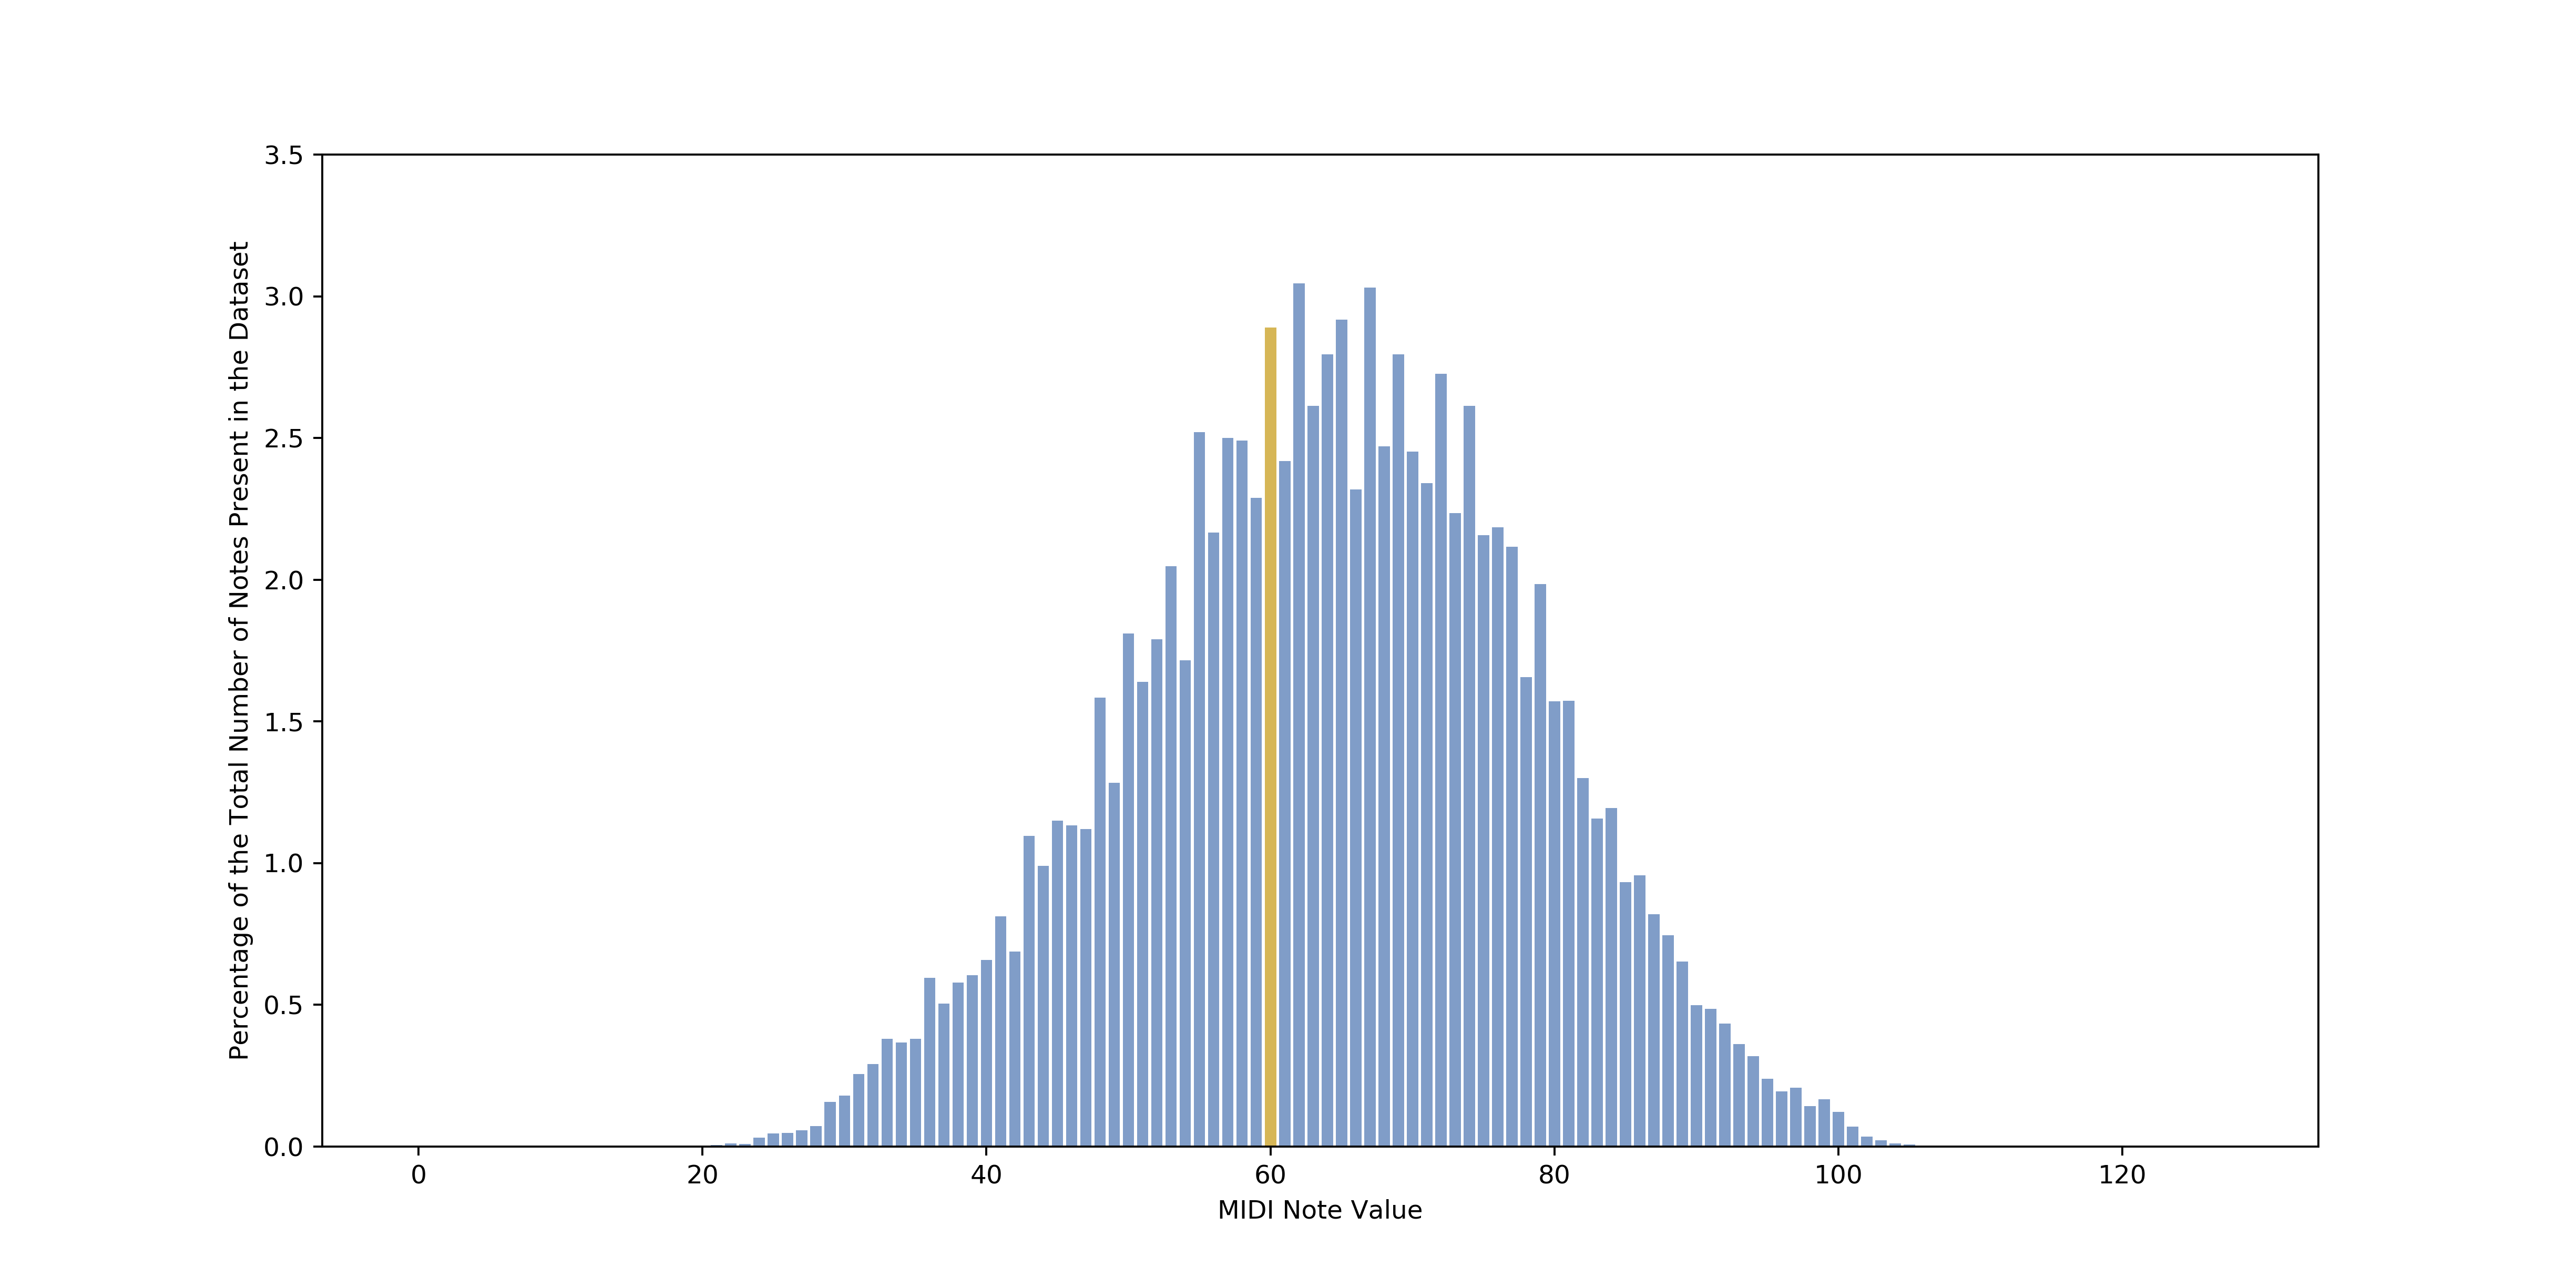
\includegraphics{Images/classicnotedistrib.png}
\caption{MIDI note value distribution of the MAESTRO dataset shown as
percentages of the total number of notes present}
\end{figure}

\begin{figure}
\centering
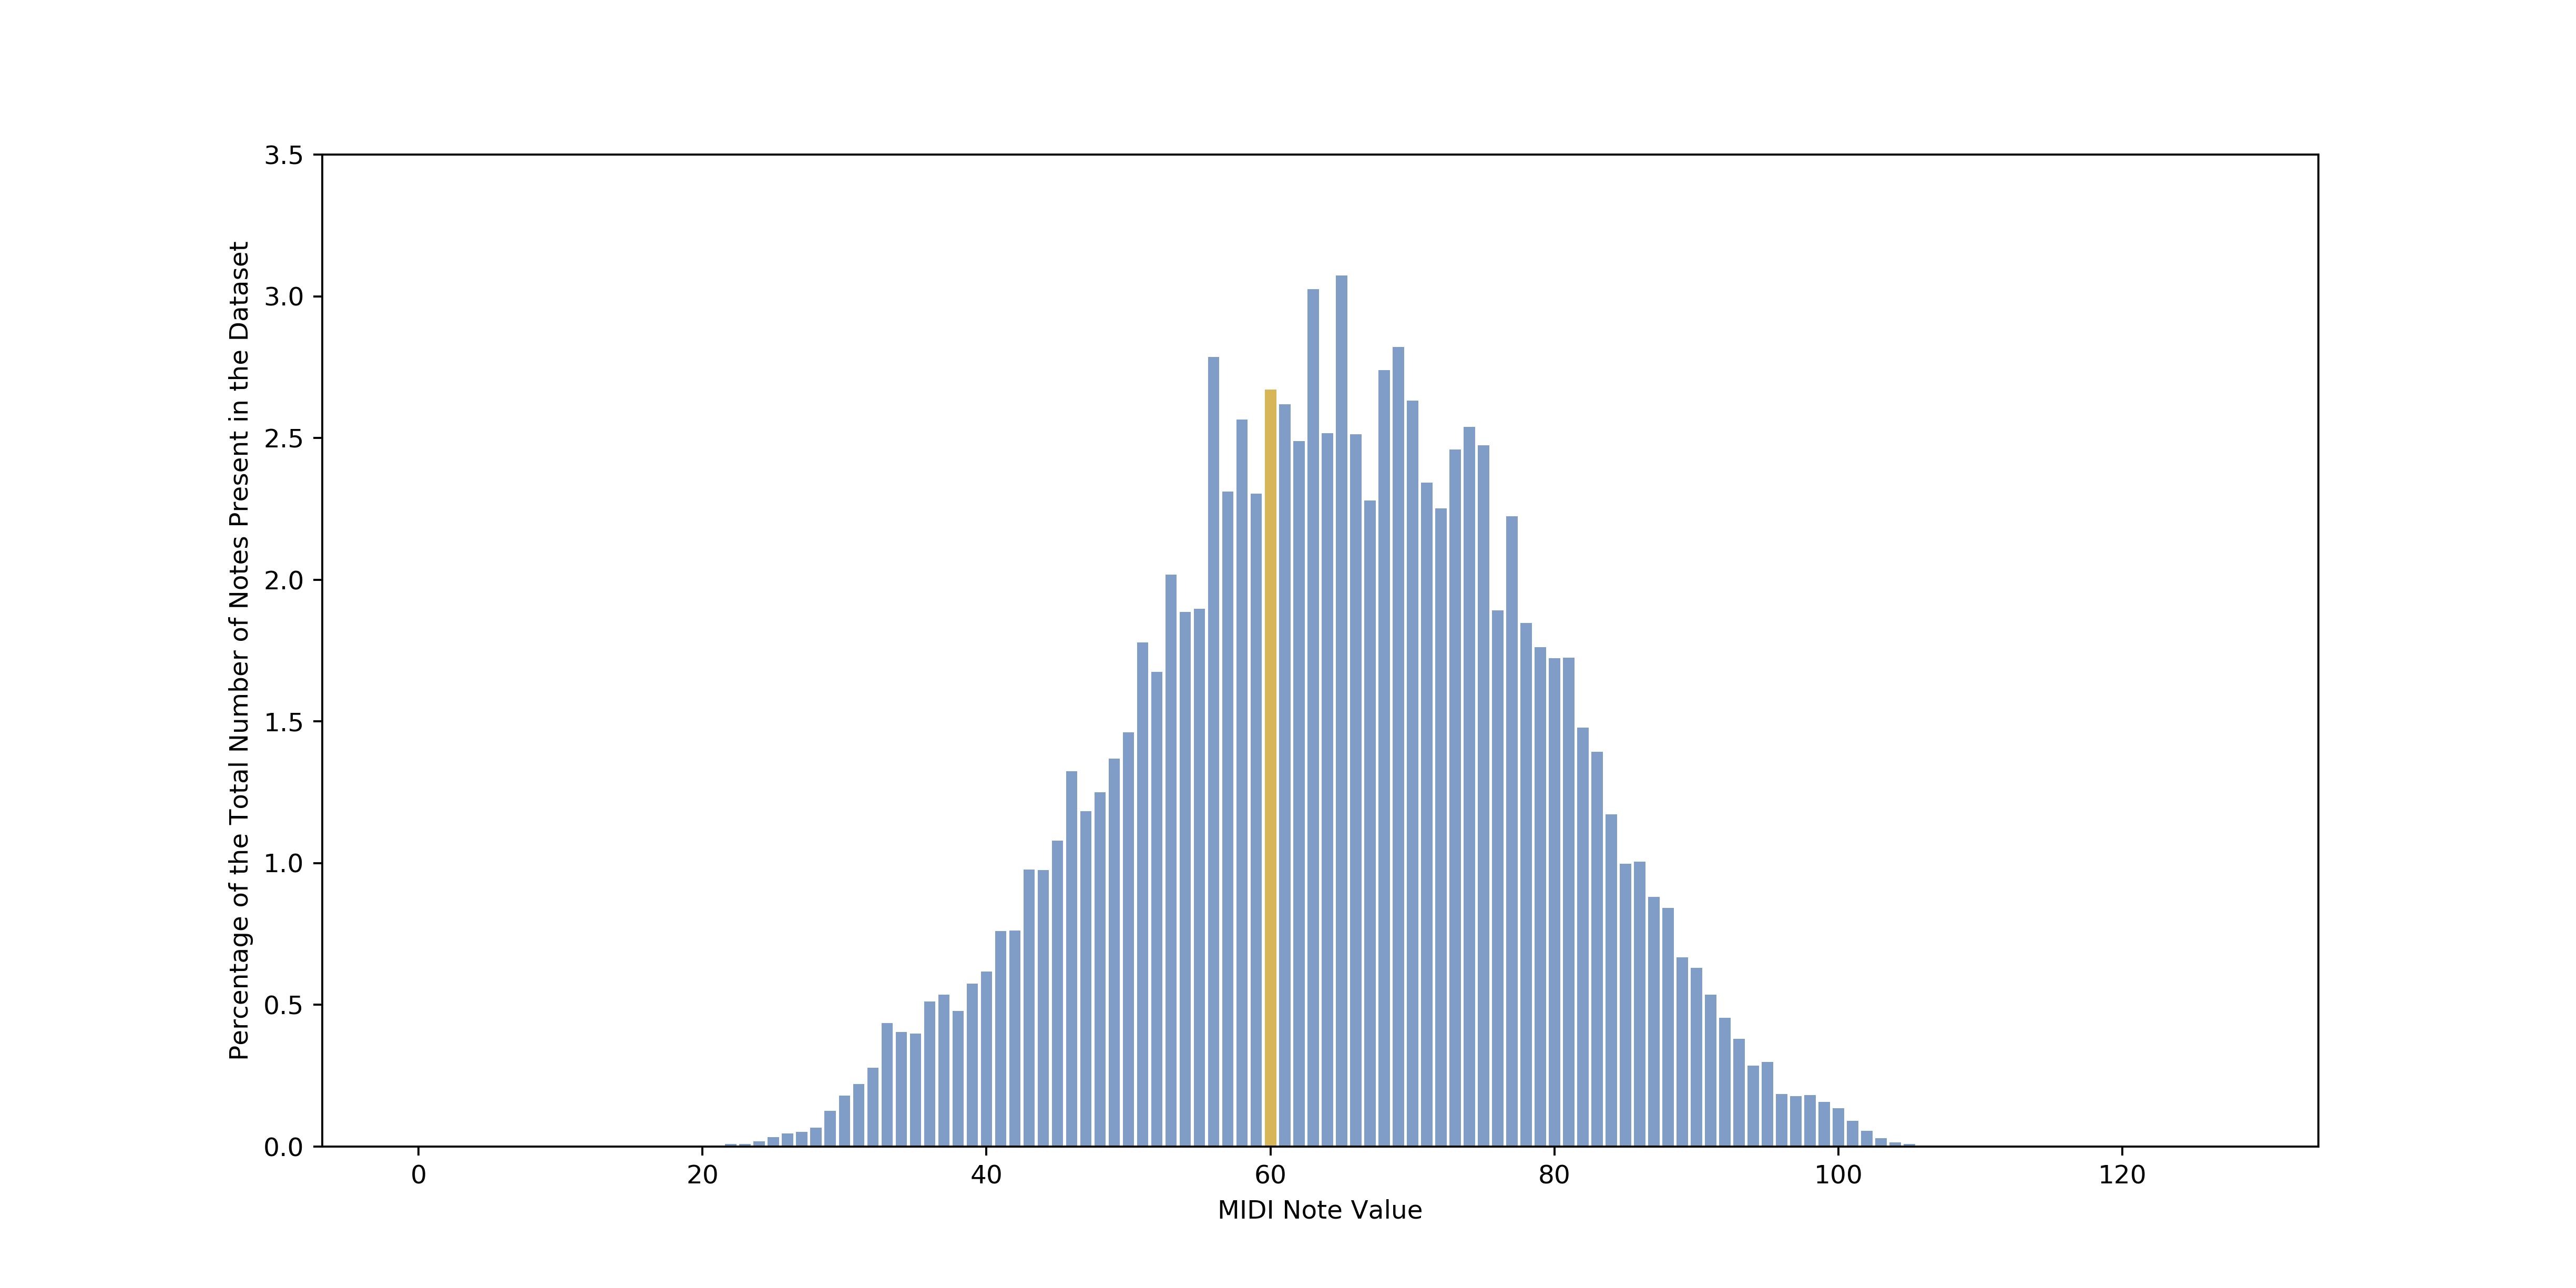
\includegraphics{Images/classicnotegendistrib.png}
\caption{MIDI note value distribution of 256 RDLSTM-generated
compositions after training on the MAESTRO dataset shown as percentages
of the total number of notes present}
\end{figure}

\begin{figure}
\centering
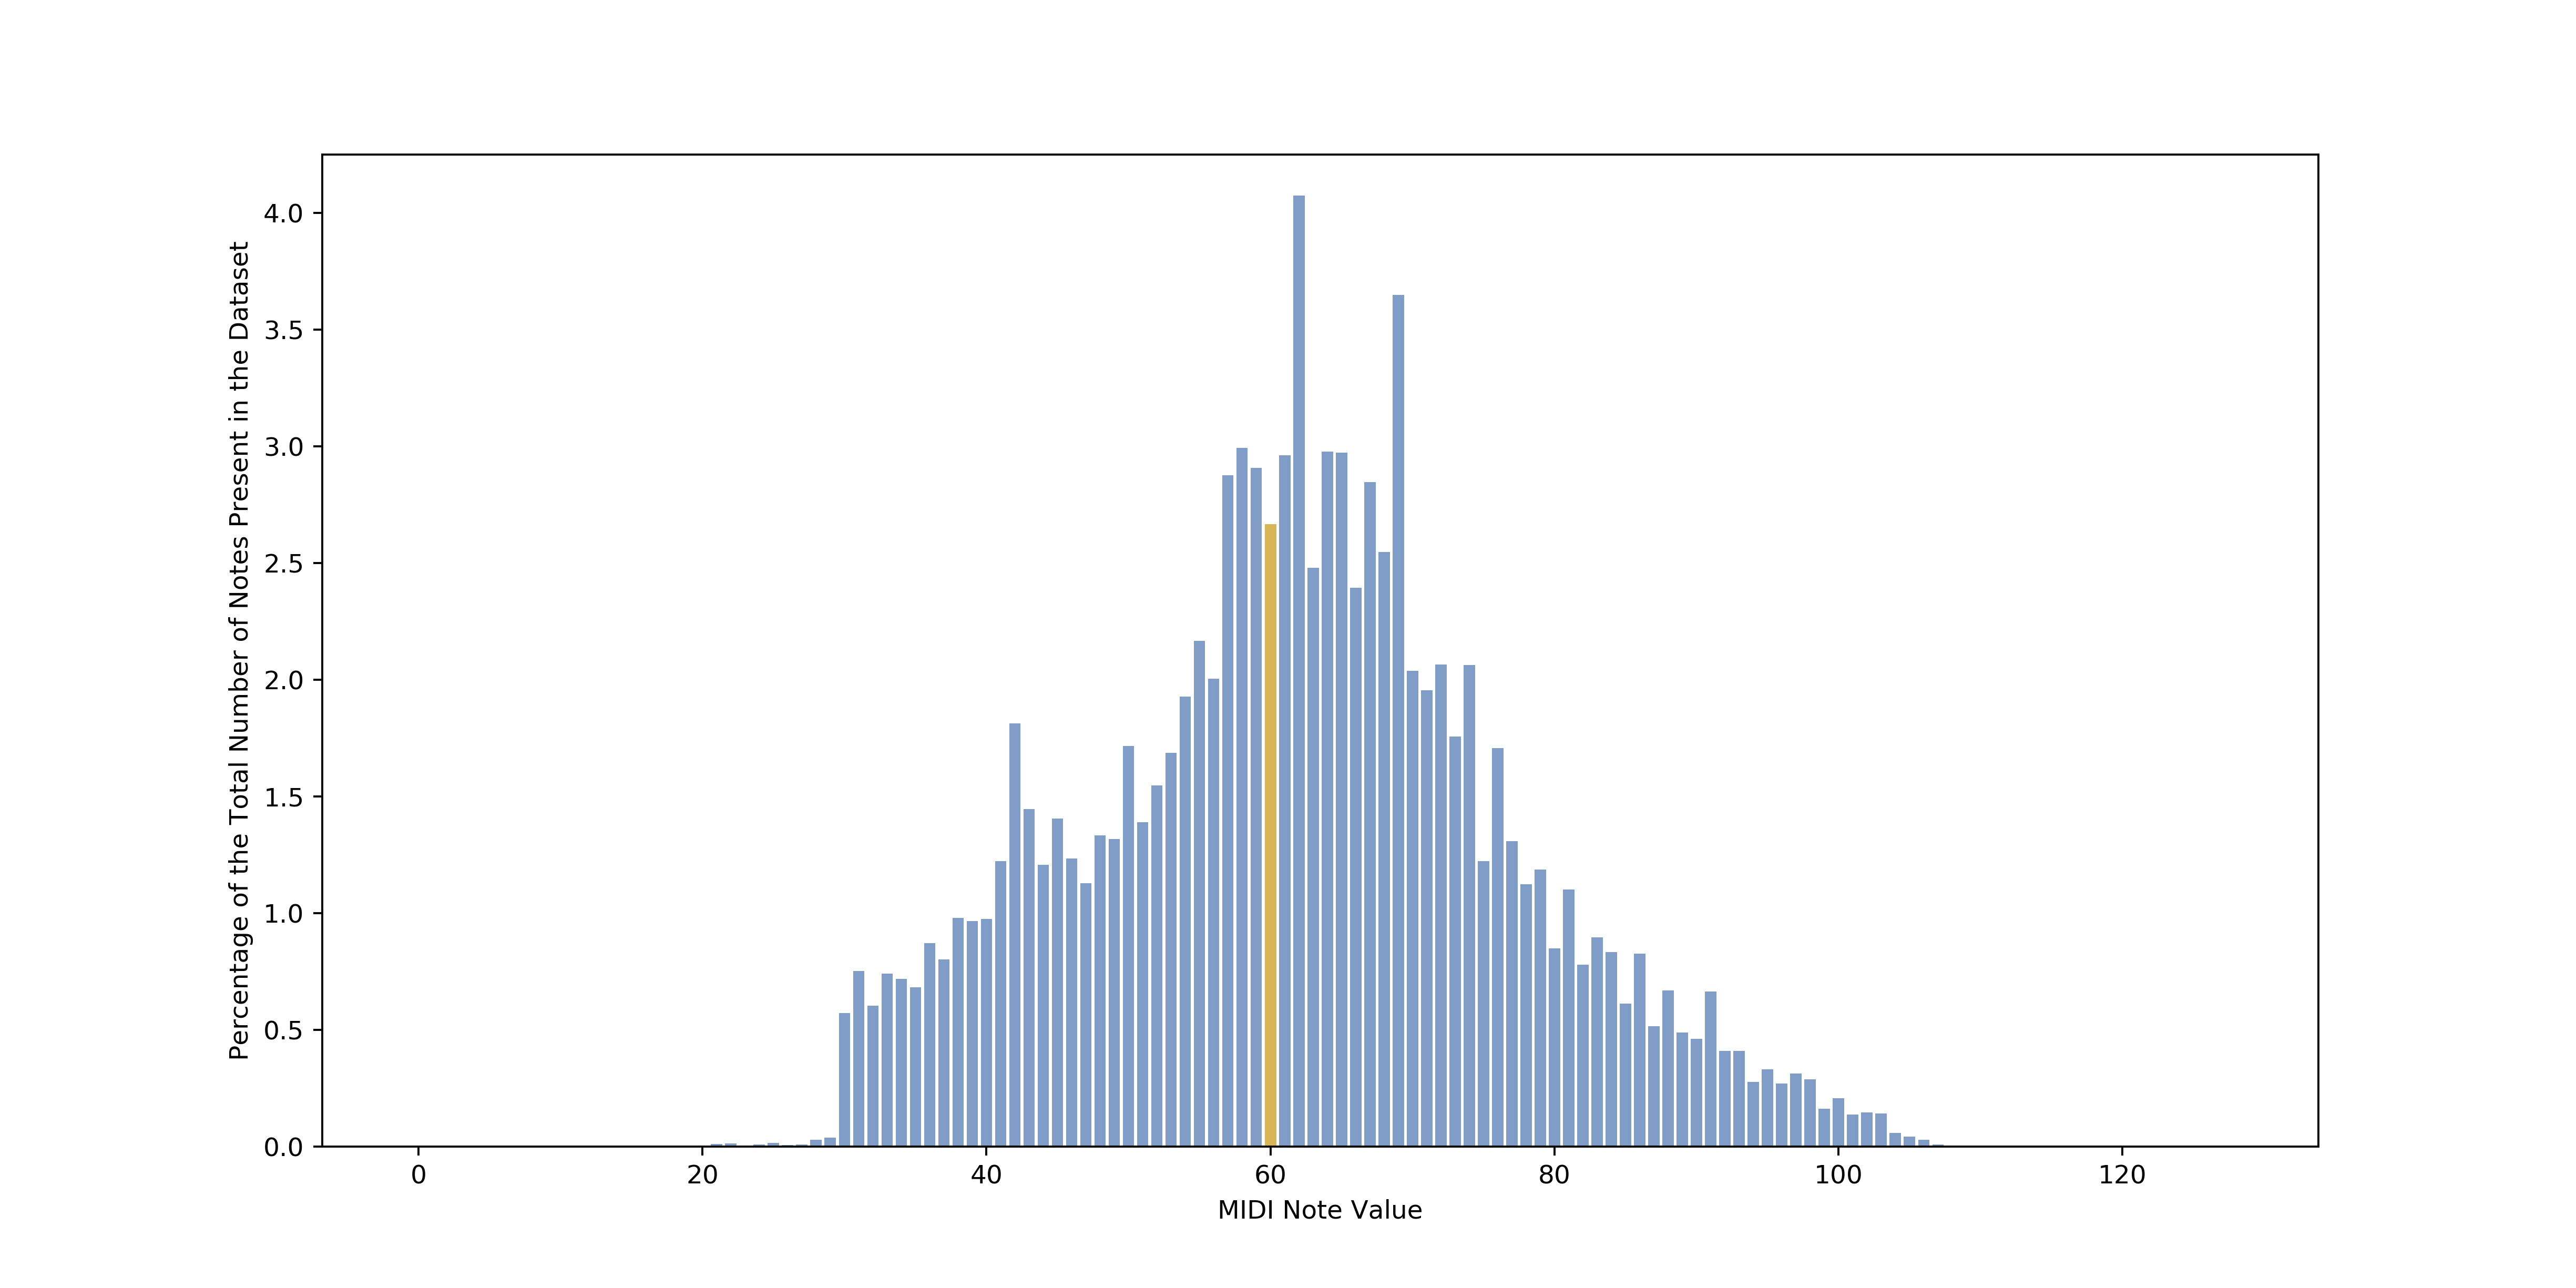
\includegraphics{Images/ambientnotedistrib.png}
\caption{MIDI note value distribution of the author-created
MIDI-transcribed ambient dataset shown as percentages of the total
number of notes present}
\end{figure}

\begin{figure}
\centering
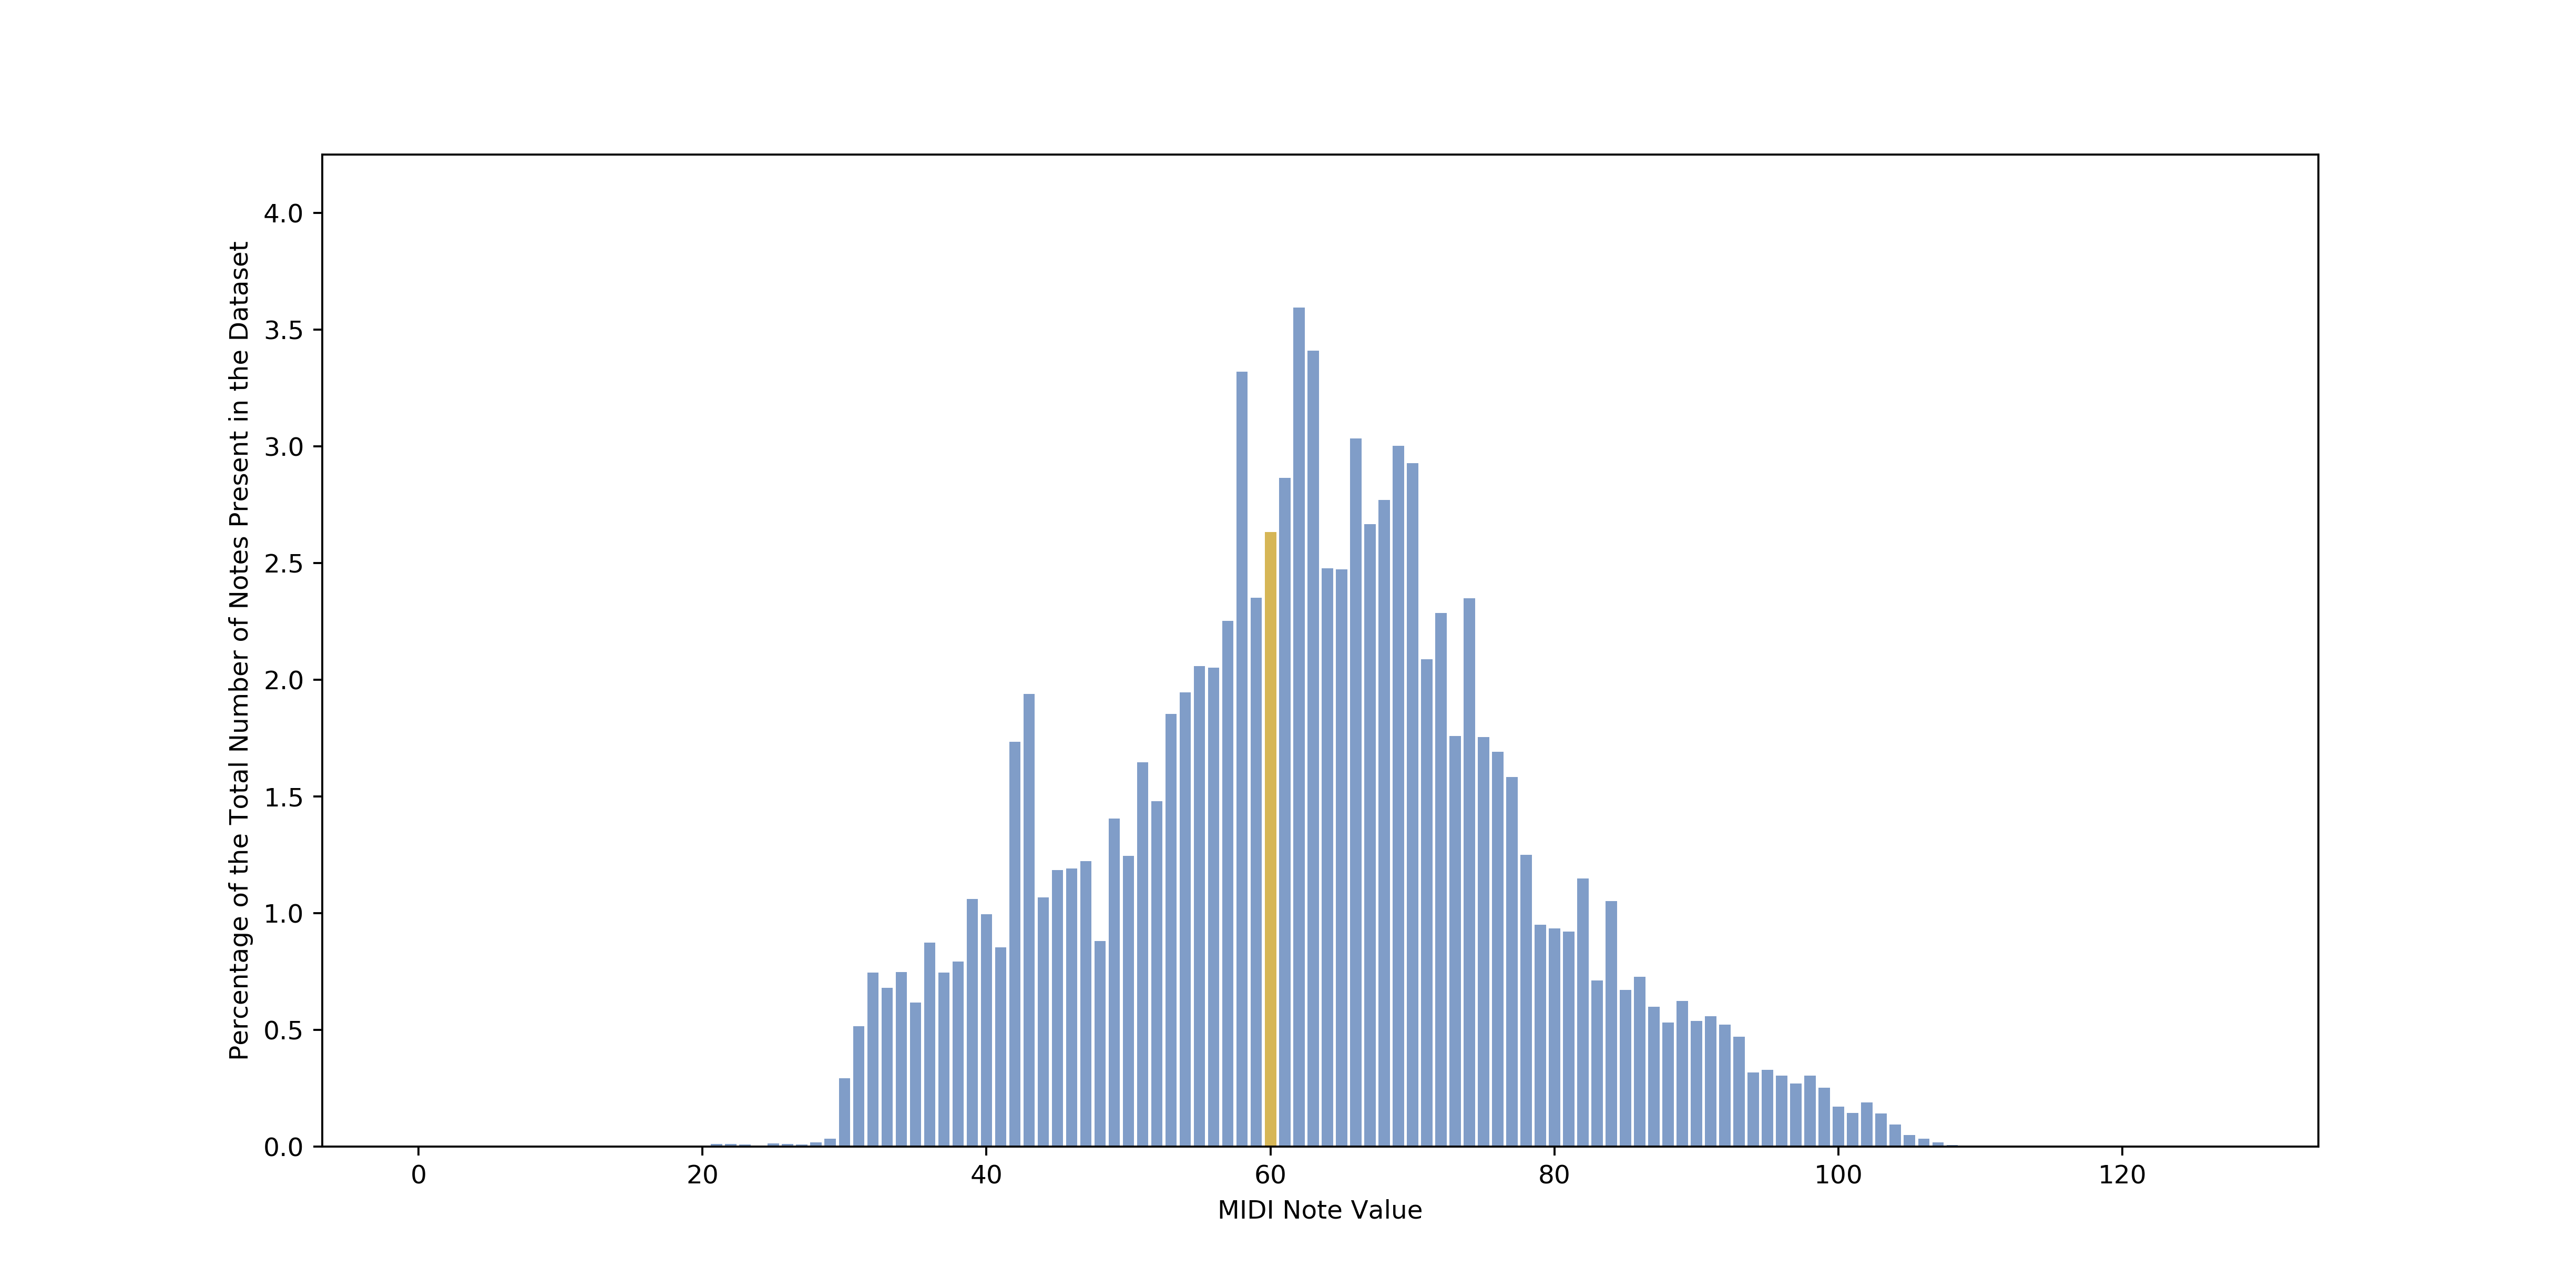
\includegraphics{Images/ambientnotegendistrib.png}
\caption{MIDI note value distribution of 256 RDLSTM-generated
compositions after training on the author-created MIDI-transcribed
ambient dataset shown as percentages of the total number of notes
present}
\end{figure}

There is also the incorporation of mood to consider. This is something
that is hard to properly assess quantitatively but is discussed at
further length \protect\hyperlink{qualitativesurveyingassessment}{in
context of the survey that was carried out}. It was found that mood did
influence the outputs to a noticeable degree and caused them to exhibit
characteristics reminiscent of the training data with similar mood
values. The influence of information provided post-generation is an
interesting concept which could extend beyond just mood to allow a user
to interact with pre-trained models in a number of ways. However, it is
proposed that a much greater dataset may be required for each of these
characteristics that are incorporated into the model so that
compositional systems can learn enough context for a user's input to
have a meaningful effect. This is because the effect of an additional
vector - in this case representing mood - may have on the model's
learning is mainly to associate certain parameters or situations with
that certain mood. This is effectively splitting the training data, or
at least applying some over-arching weighting to its elements so that a
user's input has a noticeable effect on the generated compositions.

\hypertarget{contextualised-comparisons-with-existing-solutions}{%
\subsection{Contextualised Comparisons with Existing
Solutions}\label{contextualised-comparisons-with-existing-solutions}}

In order to offer a fair comparison to previous work, the part of the
models incorporating sentiment was disabled for the duration of training
on the aforementioned ``standard'' datasets for quantitative assessment
of a model's performance in this task. The table below indicates the
average loss exhibited by the models when exposed to unseen test data
after training to validation loss convergence. The data for all other
architectures is sourced from previous work
{[}\protect\hyperlink{ref-boulanger2012modeling}{21}{]},
{[}\protect\hyperlink{ref-vohra2015modeling}{32}{]},
{[}\protect\hyperlink{ref-johnson2017generating}{33}{]}, a 20:60:20
test:train:validation split is adhered to once again. Note that the
log-likelihood performance metric shown here is simply the negative of
the cross entropy metric discussed in the
\protect\hyperlink{training}{training} section. The formulation for this
can be seen clearly by considering the formulae for both loss metrics;
note that when negative log-likelihood is used it is required that a
softmax calculation layer be placed at the end of a network in order to
create valid inputs for it.

The first and main evaluation experiment was carried out on the four
datasets with a uniform key enforced throughout (these datasets are all
in a uniform key by default). This is because most prior research did
not attempt to incorporate relative harmonics into their model as this
work does, meaning they did not generalise across different keys well at
all. Note that the architectures referred to as RDGRU and RDLSTM
(meaning Relativistic Dilated GRU / LSTM) embody the architectures where
768 units were used in each of 4 layers.

\begin{table}[H]
\centering
\caption{Log-likelihood performance during non-transposed compositional training. The table shows results from a selection of previous works’ models above the line alongside the ones created as part of this project below the line.}
\vspace{1em}
\begin{tabular}{lcccc} 
\toprule
\textbf{Model}    & \textbf{JSB Chorales} & \textbf{MuseData} & \textbf{Nottingham} & \textbf{Piano-Midi.de}  \\ 
\midrule
Random            & -61.00                & -61.00            & -61.00              & -61.00                  \\
Markovian         & -12.22                & -19.03            & -5.94               & -27.64                  \\
RBM               & -7.43                 & -9.56             & -5.25               & -10.17                  \\
NADE              & -7.19                 & -10.06            & -5.48               & -10.28                  \\
RNN               & -8.71                 & -8.13             & -4.46               & -8.37                   \\
RNN (HF)          & -8.58                 & -7.19             & -3.89               & -7.66                   \\
RNN-RBM           & -7.27                 & -9.31             & -4.72               & -9.89                   \\
RNN-RBM (HF)      & -6.27                 & -6.01             & -2.39               & -7.09                   \\
RNN-NADE          & -5.83                 & -6.74             & -2.91               & -7.48                   \\
RNN-NADE (HF)     & -5.56                 & -5.60             & -2.31               & -7.05                   \\
LSTM-NADE         & -6.00                 & -5.02             & -2.02               & -7.36                   \\
TP-LSTM-NADE      & -5.88                 & -4.32             & -1.61               & -5.44                   \\
BALSTM            & -5.05                 & -3.90             & -1.55               & -4.90                   \\
RNN-DBN           & -5.68                 & -6.28             & -2.54               & -7.15                   \\
\textbf{DBN-LSTM} & \textbf{-3.47}        & -3.91             & \textbf{-1.32}      & -4.63                   \\ 
\midrule
RDGRU (All 768)             & -3.79                 & -3.69             & -1.45               & -4.92                   \\
\textbf{RDLSTM (All 768)}   & -3.68                 & \textbf{-3.65}    & -1.36               & \textbf{-4.57}          \\
\bottomrule
\end{tabular}
\end{table}

The best loss scores are shown in bold for convenience. It can be seen
from this that the models compete with the current state-of-the-art
architectures, these are BALSTM and DBN-LSTM as mentioned in the related
work at the beginning of this report. They both incorporate
sophisticated features different to the main ones discussed here;
implying that the formulated architectures offer impressive new ideas
and results.

A ``bi-axial'' LSTM (BALSTM) architecture was recently proposed which
partially inspired the decision to try and introduce harmonic invariance
to the architectures discussed here
{[}\protect\hyperlink{ref-johnson2017generating}{33}{]}; this
architecture generalises more effectively to different keys and so was
evaluated on transposed versions of the four datasets incorporating
numerous keys by applying shifts to some of the pieces (this
transposition is done in accordance with prior discussion on musical
theory and harmonics). After some discussion with the author of this
paper, this evaluation technique could be emulated and verified
relatively easily leading to it being included in this report as well.
It can be seen that the performance of the model architectures developed
here surpass all previous work.

\begin{table}[H]
\centering
\caption{Log-likelihood performance during transposed compositional training. The table shows results from a selection of previous works’ models above the line alongside the ones created as part of this project below the line.}
\vspace{1em}
\begin{tabular}{lcccc} 
\toprule
\textbf{Model}    & \textbf{JSB Chorales} & \textbf{MuseData} & \textbf{Nottingham} & \textbf{Piano-Midi.de}  \\ 
\midrule
LSTM-NADE         & -9.04                 & -5.72             & -3.65               & -8.11                   \\
TP-LSTM-NADE      & -5.89                 & -4.32             & -1.61               & -5.44                   \\
BALSTM            & -5.08                 & -3.91             & -1.55               & -4.92                   \\
\midrule
\textbf{RDGRU (All 768)}  & -3.81                 & -3.73             & \textbf{-1.36}      & -5.01                   \\
\textbf{RDLSTM (All 768)} & \textbf{-3.67}        & \textbf{-3.66}    & -1.38               & \textbf{-4.43}          \\
\bottomrule
\end{tabular}
\end{table}

\hypertarget{qualitative-surveying-assessment}{%
\subsection{Qualitative Surveying
Assessment}\label{qualitative-surveying-assessment}}

A survey was carried out to aid in the qualitative assessment of the
models; it is important to consider human perception of the outputs due
to our ability to assess features on a local level such as quickly
noticing off-notes and timings. Additionally, humans possess an
appreciation for repeated motifs and long-term structures in music which
are difficult for a computer to detect as has been a recurring theme
throughout this report. A group of 30 participants were presented with
ten compositions of approximately two minutes in length. Half of these
compositions were inputs to the network from the MAESTRO dataset,
i.e.~human compositions. The other half were outputs of the network,
novel compositions generated by the model after being trained on
MAESTRO. Their task was simply to identify which were composed by humans
and which were composed by the model. Their average accuracy was 57\%
which is only marginally better than randomly guessing, suggesting the
models were convincing in their outputs.

Following this, the participants were asked for general thoughts on the
model and presented with generations from a variety of different
sentimental value inputs and asked to judge the impact inputted mood had
on the outputs. For this part of the survey, only around 67\% stated
that the inputted mood seemed to have any meaningful effect on the
output. This is again a positive result but indicates further work is
necessary to improve this part of the compositional system. All of them
stated that the qualitative outputs of the exhibited models (the RDGRU
and RDLSTM) were impressive not only in the domain of classical piano
but also after training on the aforementioned author-generated ambient
music dataset.

This survey reinforces the author's thoughts on the outputs of the
models. Through listening to many of the outputs, it can be seen that
the model rarely plays out of tune and often maintains a pattern or
long-term structure effectively for extended periods. The outputs are
polyphonic and harmonically complex and the temporal structure in terms
of gaps between notes is usually regular and consistent leading again to
the conclusion that the model is successfully emulating how a human
might compose a piece. Longer samples do tend to slowly diverge from
initial motifs and can begin to stutter; often gaps in playing occur at
unexpected intervals as the model seems to drift between ideas. This is
an issue reminiscent of other solutions and occurs less than in most
other work but relates to the inherent issues of these probabilistic
generative processes.

As mentioned in the \protect\hyperlink{introduction}{introduction}, one
stretch goal included the creation of a website hosting a pre-trained
model and incorporating some of the features of the survey discussed
here. Following the completion of the more challenging technical
components of this project, it would be feasible given more time for
this website to be created and utilised to facilitate a collection of
survey responses on a much larger scale via connecting with people on
the internet, provided the project gained enough traction online.

The main issues with the survey carried out for this part of the
evaluation likely revolve around the relatively small population size
meaning given more time the creation of this web application would be
desirable. As already mentioned, it was not deemed to be sufficiently
valuable in terms of the actual output of this project to justify the
time and resources spent on it, considering the main goals were
highlighted as concerning the actual compositional model rather than the
interactivity something like a web application would provide.

\hypertarget{conclusions}{%
\subsection{Conclusions}\label{conclusions}}

Taking all of this evaluation into account, it can be seen that
quantitatively the models all perform favourably when compared to
previous work. This field is a fast moving one and evidently the
application of some of the deep learning advances introduced and
justified throughout this report has a positive impact on models working
in this domain. The RDLSTM especially is a contender amongst the current
state-of-the-art approaches, especially considering this project's
emphasis on usability in terms of computational efficiency and the
optional incorporation of a user-generated training dataset. The models
fulfil all of the requirements mentioned in the first section of this
report and do so in a competitive manner. Moreover, the representation
is compact and simple whilst providing adequate details of the temporal,
harmonic and performative structures present in musical composition. The
tabulated loss metric outcomes on the standard datasets represent work
from the past few years, indicating that this problem is quickly gaining
momentum and it is likely that future work could surpass the models
discussed here, especially if features from other research surrounding
the DBN-LSTM and BALSTM were incorporated with features of this work.

The model architecture and parameter configuration settled upon is
likely to be near-optimal; there are potentially even more favourable
configurations in terms of layer count and size that would require more
time and resources to discover. The functions these networks aim to
model are exceedingly complex and it is still somewhat unclear how many
neurons might work best. Additionally, more context was seen to aid
models in performing better, whether that be provided through the
architecture as is the case here or perhaps in some further development
of the representation to include global structures such as re-occurring
chord progressions. The issue with representational changes is that it
immediately makes the model and data less accessible and versatile
across tasks. It would be interesting to also be able to input a key
into the model but it is currently unclear as to whether this simply
obscures / simplifies the overall task.

One of the main issues faced is with regards to the training data and
representation: propagation of noise or errors throughout the system
starting with MIDI transcription and any uncertainty present in the
pre-existing datasets can hinder a model's capacity to learn. As the
field of musical transcription develops it will be possible to create
much larger training datasets that would likely offer increased
performance from all musical composition models. Qualitative evaluations
of the mood parameters incorporated into the system at the point of
generation were less conclusive than the evaluation of more typical
features. It is likely that as more high-quality data becomes available,
the mood of pieces can more accurately be transferred into the models
during training and thus have a more substantial impact on the outputted
compositions post-training. Notably, the outputted pieces did include a
range of velocities and dynamics to match those present in the training
data; this builds upon the general successes observed when considering
the distribution of notes by percentage of total as presented at the
start of this section.

Despite these relative and contextual successes, it is important to
consider the fact that all machine learning models such as these
incorporate bias through their training datasets. The model architecture
itself in this case was successful by achieving independence from any
particular style or genre (a feature proven by its ability to produce
quality outputs after training with different genres of music); a future
goal could be to have a model that can be trained \emph{once} and yet
produce music spanning or even merging different styles together. This
information could be incorporated in a similar way to the mood vectors
proposed in this report. These biases mean that it is difficult for a
model to be truly inspired, as was noted by some survey participants and
the author when assessing the models composed pieces. For now, the most
effective models in this space are impressive in their ability to
masquerade as human composers, but are perhaps still lacking when
compared to the creative innovation humans are capable of.

This creativeness is the ``true'' goal that has evaded researchers for
over 100 years and it is perhaps questionable as to whether computers
could ever fully achieve it. Certainly, with more data and more complex
models it is likely that they could potentially begin to exhibit
elements of this behaviour. The models shown here already do exhibit
novel progressions and often very complex harmonic structures that some
musicians would struggle to formulate for themselves meaning the outputs
could already be utilised as musical inspiration for musicians who were
willing to filter through a lot of outputs from the models.

This eventual goal is widely accepted as aspirational and indeed
comprises a great computational challenge, the pursuit of which will
likely lead to many more interpolations and developments in deep
learning research and beyond. Relative to the goals of this project, the
overall results achieved here are impressive and satisfy the main
requirements that were outlined in the specification and introduction.
The two previously highlighted stretch goals were not met but it is
estimated that following this work, they would be relatively trivial to
implement given more resources (especially in terms of hosting and
knowledge on sentimental analysis of images).

\hypertarget{future-work}{%
\section{Future Work}\label{future-work}}

\hypertarget{improved-data-collection-and-corpus-creation}{%
\subsection{Improved Data Collection and Corpus
Creation}\label{improved-data-collection-and-corpus-creation}}

As has already been alluded to, perhaps the biggest issue faced
throughout this project has been one of data. New architectures were
developed and tested iteratively but all of them faced similar
limitations due to a lack of data. The model itself proved to be close
to state-of-the-art through its training performance and quantitative
evaluation. However, many of the pieces still seemed to leave something
to be desired; especially when the created ambient corpus was used.
These models actually tend to struggle more with larger datasets if the
size is accompanied by the introduction of a larger amount of variance;
the eventual aim is to build models capable of dealing with and
effectively interpreting this variance as creative opportunity, but
currently leads to the requirement of long training times and complex
models. This is why there is emphasis on not only the size of training
data, but also the quality and coherence of it as a corpus. It is also
why most other work focusses on relatively homogenous datasets such as
Bach chorales and so on.

OpenAI recently published a break-through paper surrounding their GPT-2
model {[}\protect\hyperlink{ref-radford2018language}{69}{]} which has
reached new heights in language modelling and generation. The team cites
much of the improvement as being a result of the scale and quality of
their training data as well as their available resources and
computational capacity. In many cases, the simple introduction of better
data and resources in this way are the key to breaking previous
benchmarks in the deep learning space.

Building on this point, the mood representation is currently somewhat
lacking due to a lack of data and uncertainty in the sentiment analysis
method that was applied. Advances in sentiment analysis could allow for
a more comprehensive and ultimately more informative mood representation
to be formulated.

Access to higher-quality or instrument specific data could also allow
for an attempt at the tying of multiple networks together that would
each focus on a different component of composition. For example, one
network could build chords, another melody, and another be trained on
drum patterns to produce percussion elements for a composition. It would
be challenging to link models to effectively achieve this but would
certainly be a break-through in terms of producing outputs beyond those
discussed here which must be manually separated into different virtual
instruments if that is desired (this is the reason classical piano
pieces involving a single instrument are typically used as training data
for all exiting work which does not effectively make any separation by
instrument).

\hypertarget{sentimental-input-from-images}{%
\subsection{Sentimental Input from
Images}\label{sentimental-input-from-images}}

As was discussed in this project's specification; and subsequently
checked in the progress report, aiming to implement sentimental analysis
of an image proved to be perhaps beyond the reasonable scope of a third
year project of this time-frame. The ideas were explored and even
utilised to a certain extent via the influence convolutional neural
networks (commonly applied to image analysis) had on the architectures
discussed here. However, the work itself has been done countless times
before and thus was given less gravity than the compositional part of
this project from the start. It was decided that spending a greater
portion of time on the compositional components of the project would be
more beneficial and impactful, leading to this remaining a stretch goal
for potential future work. A mood representation was defined and
incorporated successfully into the model meaning it would be a simple
matter of wiring up a solution once an appropriate image analysis tool
was developed or found to provide sentimental input from images.

\hypertarget{alternative-architectures}{%
\subsection{Alternative Architectures}\label{alternative-architectures}}

Some other recent developments in the space of recurrent units could
offer improvements to the current architecture; most of these were
either tried and discarded or are still too theoretical to practically
implement and optimise to make them a viable alternative to LSTMs etc.
All of the ones mentioned here are deemed to be `ones to watch' in the
sense that with some further development they could compete with or even
surpass all current models.

Statistical Recurrent Units
{[}\protect\hyperlink{ref-oliva2017statistical}{70}{]} substitute the
gates of GRUs and LSTMs with moving averages of a selection of recurrent
statistics. They have already achieved promising results in the task of
musical composition but were not found to be significantly better than
LSTMs and GRUs on their own. As SRUs gain traction and become optimised
they may become a viable alternative as it is provable through
differential equations that they can effectively mitigate vanishing /
exploding gradients and could potentially achieve similar results to
other units with significantly simpler parameter sets.

Variational Auto-Encoders
{[}\protect\hyperlink{ref-roberts2017hierarchical}{71}{]} and Neural
Turing Machines {[}\protect\hyperlink{ref-graves2014neural}{72}{]} again
build on the issues of RNNs and have features which would make them
worth applying to musical composition. Google's Magenta team published a
paper during the course of this project that pursued similar goals to
those laid out here: they utilised VAEs to combat long-term coherence
issues and had success in doing so
{[}\protect\hyperlink{ref-roberts2018hierarchical}{73}{]}. It would be
interesting to look at applying concepts used in these recent
publications and the aforementioned state-of-the-art DBN-LSTM to the
ground breached here in terms of harmonic invariance and dilation. Both
of these competitive solutions are recent (in the case of Google's VAEs
too recent to even consider exploring in full) and both aim to tackle
very similar issues to the ones discussed here but in different ways;
this adds credibility to the purpose and methodology followed in this
report in terms of its contribution to progressing musical composition
as an area in deep learning research.

A potential extension of this project would be to integrate dilation
more fully into a custom recurrent unit specialised in determining
musical temporal and harmonic structures. The exhibited research and
implementation could indicate the potential of a recurrent unit which
more fully integrates the concepts of convolutional neural networks into
its design and formulation.

\hypertarget{performance-and-interactivity}{%
\subsection{Performance and
Interactivity}\label{performance-and-interactivity}}

This project proves that additional features can effectively be
incorporated into a model architecture by way of the incorporation of
sentiment. A natural extension of this would be to provide additional
ways to interact with the model at the point of generation through
giving a user the chance to manually inspire the model. This could
potentially be as intuitive as allowing a user to play a short number of
notes or chords and have these set the initial weightings for the
network, which would presumably go on to compose a whole piece from
these starting conditions. This would certainly be possible given a
greater corpus of training data to allow for the model to have a greater
understanding of shorter inputs; allowing for musicians to use the model
creatively in terms of inputting short ideas into it and exploring its
responses.

Many of the Magenta team's efforts since the launch of the interactive
TensorFlow JavaScript platform have incorporated ideas such as these; it
is relatively simple to hook up a MIDI interface into the model such
that it could receive input in a similar way to some of the existing
Magenta models.

In order to further build upon the user experience of this project, a
simple web app could be built to contribute to a larger population size
for the \protect\hyperlink{qualitativesurveryingmethod}{surveying
method} described in the evaluation section. The web app would allow for
a user to input a mood either by setting the Circumplex parameters
manually or potentially tying in the use of an uploaded image or even
NLU to analyse the mood of a sentence and then feed this into the model
to generate a piece. The hosting of a pre-trained model would be
relatively simple to achieve and again was not deemed to be of
sufficient value to justify the time and resource cost during this
project as it was not key to the initially laid out requirements.
Despite this, it could potentially gain traction online and provide a
much larger sample size for automated collection of qualitative
assessment data regarding the model.

\hypertarget{synthesiser-parameters}{%
\subsection{Synthesiser Parameters}\label{synthesiser-parameters}}

One of the advantages of training a model with MIDI data and
subsequently generating it is the flexibility and portability MIDI
offers as a format. The generated sequences may be used to sequence
notes on almost any synthesiser (probably all but those produced before
around 1980) with the required interfacing as well as all digitally
synthesised and sampled instruments. Other researchers have successfully
trained a model to change parameters of a synthesiser during live
performance based on a musician's input and learned preferences
{[}\protect\hyperlink{ref-sommer2014towards}{74}{]}.

Moving forward this would be an excellent way to add another dimension
to the project's generated compositions; existing studies into the
sentiments behind different timbres and urgency or latency introduced by
manipulations of note attack-delay-sustain-release parameters could form
a basis of some quantitative assessment of the results. This could
essentially be an extension of the influence a user's input could have
on the model, influencing the output through affecting the choice of
parameter programming for the synthesiser / virtual instrument used to
play the outputted compositions as well as the composition itself.

\hypertarget{authors-assessment-of-the-project}{%
\section{Author's Assessment of the
Project}\label{authors-assessment-of-the-project}}

It is evident from the work discussed that the level of technical
achievement this project encompasses is beyond the scope of the current
undergraduate curriculum. Much of the work is of a high level for a
third year project and involved significant time investment in order to
learn additional advanced material with which to accomplish the goals of
the project. From this perspective, the project has been a fulfilling
and excellent learning experience for me as the author; as well as
offering the chance to fully immerse oneself in research for the first
time and assure my own relationship with it moving forward.

The use of neural networks and deep learning is adherent to the
description of my degree; probabilistic sequence generation is certainly
relevant in almost all aspects to the statistical and computational
nature of the BSc in Data Science. The project illustrates domain
knowledge spanning multiple fields relevant to data science and involved
numerous challenging components from research, theoretical, technical
and engineering perspectives. The implementation of cutting-edge
recurrent units and algorithms for deep learning required sufficient
knowledge of mathematics and statistics especially when drawing
comparisons between probabilistic processes exhibiting Markovian and
recurrent behaviours.

One of the biggest challenges faced throughout arose due to the initial
design of the project: having a lot of avenues to explore is time
consuming but was necessary in this instance due to a lack of the prior
understanding required to make these judgements from the start.
Decisions were reached however and led to a satisfactory outcome when
put in context with the initial objectives and requirements of the
project. The initial time spent on research proved fruitful due to the
relatively ill-defined landscape surrounding the problem: there is no
current clear leader in the space, and it could be said that a
completely satisfactory solution still seems somewhat out of reach. It
is clear however that research in recent years has considerably improved
upon past attempts and the evaluation of the work provides a promising
view on the future of automated composition.

It is hoped that this work forms a relatively robust and
all-encompassing summary of not only the outputs of the project, but the
work and context involved in achieving it. There is tangible value
present for other academics and students to aid in any further
contributions to this fast-moving field. Musical composition as
mentioned is a sufficiently complex task to fully leverage some of the
more advanced deep learning and sequential modelling techniques which
are currently of interest in academia; this work shows their potential
applications as well as hopefully contributing to their further
development.

The incorporation of mood is perhaps the initial limitation an observer
may encounter in terms of the initial goals of the project. As a proof
of concept though it has been shown that the model is flexible to the
addition of inputs beyond just MIDI data, also including augmentation
using velocity and dynamics. Training times and the overall quantitative
and qualitative performance were satisfactory; the conclusions portray
success in most areas of the project whilst being mindful of its initial
goals and scope.

\hypertarget{references}{%
\section*{References}\label{references}}
\addcontentsline{toc}{section}{References}

\hypertarget{refs}{}
\leavevmode\hypertarget{ref-nierhaus2009algorithmic}{}%
{[}1{]} G. Nierhaus, \emph{Algorithmic composition: Paradigms of
automated music generation}. Springer Science \& Business Media, 2009.

\leavevmode\hypertarget{ref-deng2014deep}{}%
{[}2{]} L. Deng, D. Yu, and others, ``Deep learning: Methods and
applications,'' \emph{Foundations and Trends in Signal Processing}, vol.
7, nos. 3 -- 4, pp. 197--387, 2014.

\leavevmode\hypertarget{ref-najafabadi2015deep}{}%
{[}3{]} M. M. Najafabadi, F. Villanustre, T. M. Khoshgoftaar, N. Seliya,
R. Wald, and E. Muharemagic, ``Deep learning applications and challenges
in big data analytics,'' \emph{Journal of Big Data}, vol. 2, no. 1, p.
1, 2015.

\leavevmode\hypertarget{ref-goodfellow2016deep}{}%
{[}4{]} I. Goodfellow, Y. Bengio, and A. Courville, \emph{Deep
learning}. MIT press, 2016.

\leavevmode\hypertarget{ref-luque2009stochastic}{}%
{[}5{]} S. Luque, ``The stochastic synthesis of iannis xenakis,''
\emph{Leonardo Music Journal}, pp. 77--84, 2009.

\leavevmode\hypertarget{ref-eck2002finding}{}%
{[}6{]} D. Eck and J. Schmidhuber, ``Finding temporal structure in
music: Blues improvisation with lstm recurrent networks,'' in
\emph{Proceedings of the 12th ieee workshop on neural networks for
signal processing}, 2002, pp. 747--756.

\leavevmode\hypertarget{ref-gers1999learning}{}%
{[}7{]} F. A. Gers, J. Schmidhuber, and F. Cummins, ``Learning to
forget: Continual prediction with lstm,'' 1999.

\leavevmode\hypertarget{ref-magenta}{}%
{[}8{]} \relax Google Brain Team, ``TensorFlow Magenta.''
\url{https://github.com/tensorflow/magenta}.

\leavevmode\hypertarget{ref-huang2018improved}{}%
{[}9{]} C.-Z. A. Huang \emph{et al.}, ``An improved relative
self-attention mechanism for transformer with application to music
generation,'' \emph{arXiv preprint arXiv:1809.04281}, 2018.

\leavevmode\hypertarget{ref-oord2016wavenet}{}%
{[}10{]} A. van den Oord \emph{et al.}, ``WaveNet: A generative model
for raw audio.'' 2016.

\leavevmode\hypertarget{ref-mediumkylemcdonald}{}%
{[}11{]} K. McDonald, ``Neural nets for generating music.'' \\
\url{https://medium.com/artists-and-machine-intelligence/neural-nets-for-generating-music-f46dffac21c0}.

\leavevmode\hypertarget{ref-libdlmusic}{}%
{[}12{]} Y. Bayle, ``Deep learning for music chronicle.'' \\
\url{https://github.com/ybayle/awesome-deep-learning-music}.

\leavevmode\hypertarget{ref-dai2018music}{}%
{[}13{]} S. Dai, Z. Zhang, and G. G. Xia, ``Music style transfer: A
position paper,'' \emph{arXiv preprint arXiv:1803.06841}, 2018.

\leavevmode\hypertarget{ref-hawthorne2017onsets}{}%
{[}14{]} C. Hawthorne \emph{et al.}, ``Onsets and frames: Dual-objective
piano transcription,'' \emph{arXiv preprint arXiv:1710.11153}, 2017.

\leavevmode\hypertarget{ref-bereketai}{}%
{[}15{]} M. Bereket and K. Shi, ``An ai approach to automatic natural
music transcription.''

\leavevmode\hypertarget{ref-sigtia2016end}{}%
{[}16{]} S. Sigtia, E. Benetos, and S. Dixon, ``An end-to-end neural
network for polyphonic piano music transcription,'' \emph{IEEE/ACM
Transactions on Audio, Speech, and Language Processing}, vol. 24, no. 5,
pp. 927--939, 2016.

\leavevmode\hypertarget{ref-sarnatskyi2017music}{}%
{[}17{]} V. Sarnatskyi, V. Ovcharenko, M. Tkachenko, S. Stirenko, Y.
Gordienko, and A. Rojbi, ``Music transcription by deep learning with
data and" artificial semantic" augmentation,'' \emph{arXiv preprint
arXiv:1712.03228}, 2017.

\leavevmode\hypertarget{ref-waon}{}%
{[}18{]} K. Ichiki, ``WaoN: A wave-to-notes transcriber.''
\url{http://waon.sourceforge.net}.

\leavevmode\hypertarget{ref-maestro2018}{}%
{[}19{]} C. Hawthorne \emph{et al.}, ``Enabling factorized piano music
modeling and generation with the maestro dataset,'' \emph{arXiv preprint
arXiv:1810.12247}. 2018.

\leavevmode\hypertarget{ref-ccarh}{}%
{[}20{]} S. University, ``Centre for computer assisted research in the
humanities.'' \\
\url{http://www.ccarh.org}.

\leavevmode\hypertarget{ref-boulanger2012modeling}{}%
{[}21{]} N. Boulanger-Lewandowski, Y. Bengio, and P. Vincent, ``Modeling
temporal dependencies in high-dimensional sequences: Application to
polyphonic music generation and transcription,'' \emph{arXiv preprint
arXiv:1206.6392}, 2012.

\leavevmode\hypertarget{ref-alextavgen}{}%
{[}22{]} A. Tavgen, ``How we made music using neural networks.'' \\
\url{https://medium.com/@ATavgen/how-we-made-music-using-neural-networks-449a62b8a332}.

\leavevmode\hypertarget{ref-karpathy}{}%
{[}23{]} A. Karpathy, ``The unreasonable effectiveness of recurrent
neural networks.'' \\
\url{http://karpathy.github.io/2015/05/21/rnn-effectiveness/}.

\leavevmode\hypertarget{ref-magentamodels}{}%
{[}24{]} \relax Google Brain Team, ``Magenta - Collection of Model
Architectures.'' \\
\url{https://github.com/tensorflow/magenta/tree/master/magenta/models/}.

\leavevmode\hypertarget{ref-yang2017midinet}{}%
{[}25{]} L.-C. Yang, S.-Y. Chou, and Y.-H. Yang, ``MidiNet: A
convolutional generative adversarial network for symbolic-domain music
generation,'' \emph{arXiv preprint arXiv:1703.10847}, 2017.

\leavevmode\hypertarget{ref-hilschermusic}{}%
{[}26{]} M. Hilscher and N. Shahroudi, ``Music generation from midi
datasets.''

\leavevmode\hypertarget{ref-wyse2018real}{}%
{[}27{]} L. Wyse, ``Real-valued parametric conditioning of an rnn for
interactive sound synthesis,'' \emph{arXiv preprint arXiv:1805.10808},
2018.

\leavevmode\hypertarget{ref-kim2016deepjazz}{}%
{[}28{]} J.-S. Kim, ``DeepJazz.''
\url{https://github.com/jisungk/deepjazz}, 2016.

\leavevmode\hypertarget{ref-brunner2017jambot}{}%
{[}29{]} G. Brunner, Y. Wang, R. Wattenhofer, and J. Wiesendanger,
``JamBot: Music theory aware chord based generation of polyphonic music
with lstms,'' in \emph{2017 ieee 29th international conference on tools
with artificial intelligence (ictai)}, 2017, pp. 519--526.

\leavevmode\hypertarget{ref-kotecha2018generating}{}%
{[}30{]} N. Kotecha and P. Young, ``Generating music using an lstm
network,'' \emph{arXiv preprint arXiv:1804.07300}, 2018.

\leavevmode\hypertarget{ref-colombo2018bachprop}{}%
{[}31{]} F. Colombo and W. Gerstner, ``BachProp: Learning to compose
music in multiple styles,'' \emph{arXiv preprint arXiv:1802.05162},
2018.

\leavevmode\hypertarget{ref-vohra2015modeling}{}%
{[}32{]} R. Vohra, K. Goel, and J. Sahoo, ``Modeling temporal
dependencies in data using a dbn-lstm,'' in \emph{2015 ieee
international conference on data science and advanced analytics (dsaa)},
2015, pp. 1--4.

\leavevmode\hypertarget{ref-johnson2017generating}{}%
{[}33{]} D. D. Johnson, ``Generating polyphonic music using tied
parallel networks,'' in \emph{International conference on evolutionary
and biologically inspired music and art}, 2017, pp. 128--143.

\leavevmode\hypertarget{ref-cho2014learning}{}%
{[}34{]} K. Cho \emph{et al.}, ``Learning phrase representations using
rnn encoder-decoder for statistical machine translation,'' \emph{arXiv
preprint arXiv:1406.1078}, 2014.

\leavevmode\hypertarget{ref-ebciouglu1988expert}{}%
{[}35{]} K. Ebcioğlu, ``An expert system for harmonizing four-part
chorales,'' \emph{Computer Music Journal}, vol. 12, no. 3, pp. 43--51,
1988.

\leavevmode\hypertarget{ref-cruz1998learning}{}%
{[}36{]} P. P. Cruz-Alcázar and E. Vidal-Ruiz, ``Learning regular
grammars to model musical style: Comparing different coding schemes,''
in \emph{International colloquium on grammatical inference}, 1998, pp.
211--222.

\leavevmode\hypertarget{ref-cope1996experiments}{}%
{[}37{]} D. Cope and M. J. Mayer, \emph{Experiments in musical
intelligence}, vol. 12. AR editions Madison, 1996.

\leavevmode\hypertarget{ref-spangler1998bach}{}%
{[}38{]} R. R. Spangler, R. M. Goodman, and J. Hawkins, ``Bach in a
box-real-time harmony,'' in \emph{Advances in neural information
processing systems}, 1998, pp. 957--963.

\leavevmode\hypertarget{ref-sturm2018let}{}%
{[}39{]} B. Sturm and O. Ben-Tal, ``Let's have another gan ainm: An
experimental album of irish traditional music and computer-generated
tunes.'' 2018.

\leavevmode\hypertarget{ref-mkofler}{}%
{[}40{]} M. Kofler, ``Deep Learning with TensorFlow.'' \\
\url{https://towardsdatascience.com/deep-learning-with-tensorflow-part-3-music-and-text-generation-8a3fbfdc5e9b}.

\leavevmode\hypertarget{ref-asimovinst}{}%
{[}41{]} F. Brinkkemper, ``Analysing Six Deep Learning Tools for Music
Generation.'' \\
\url{http://www.asimovinstitute.org/analyzing-deep-learning-tools-music/}.

\leavevmode\hypertarget{ref-specification}{}%
{[}42{]} H. Wilde, ``Composing soundscapes using machine learning and
user input,'' \emph{Project Specification}..

\leavevmode\hypertarget{ref-warwickcomputenodes}{}%
{[}43{]} \relax Warwick University, ``Compute Nodes.'' \\
\url{https://warwick.ac.uk/fac/sci/dcs/intranet/user_guide/compute_nodes}.

\leavevmode\hypertarget{ref-deepsent}{}%
{[}44{]} M. Chen, ``DeepSent.''
\url{https://github.com/muchen2/DeepSent}.

\leavevmode\hypertarget{ref-klapuri2004automatic}{}%
{[}45{]} A. P. Klapuri, ``Automatic music transcription as we know it
today,'' \emph{Journal of New Music Research}, vol. 33, no. 3, pp.
269--282, 2004.

\leavevmode\hypertarget{ref-gerhard2003pitch}{}%
{[}46{]} D. Gerhard, \emph{Pitch extraction and fundamental frequency:
History and current techniques}. Department of Computer Science,
University of Regina Regina, Canada, 2003.

\leavevmode\hypertarget{ref-mido}{}%
{[}47{]} O. M. Bjørndalen and R. Binkys, ``Mido python package.'' \\
\url{https://mido.readthedocs.io/en/latest/index.html}.

\leavevmode\hypertarget{ref-performance-rnn-2017}{}%
{[}48{]} I. Simon and S. Oore, ``Performance rnn: Generating music with
expressive timing and dynamics,'' \emph{Magenta Blog}.
\url{https://magenta.tensorflow.org/performance-rnn}, 2017.

\leavevmode\hypertarget{ref-russell1980circumplex}{}%
{[}49{]} J. A. Russell, ``A circumplex model of affect.'' \emph{Journal
of personality and social psychology}, vol. 39, no. 6, p. 1161, 1980.

\leavevmode\hypertarget{ref-logan2000mel}{}%
{[}50{]} B. Logan and others, ``Mel frequency cepstral coefficients for
music modeling.'' in \emph{ISMIR}, 2000, vol. 270, pp. 1--11.

\leavevmode\hypertarget{ref-baum1966}{}%
{[}51{]} L. E. Baum and T. Petrie, ``Statistical inference for
probabilistic functions of finite state markov chains,'' \emph{Ann.
Math. Statist.}, vol. 37, no. 6, pp. 1554--1563, Dec. 1966 {[}Online{]}.
Available: \url{https://doi.org/10.1214/aoms/1177699147}

\leavevmode\hypertarget{ref-werbos1990backpropagation}{}%
{[}52{]} P. J. Werbos and others, ``Backpropagation through time: What
it does and how to do it,'' \emph{Proceedings of the IEEE}, vol. 78, no.
10, pp. 1550--1560, 1990.

\leavevmode\hypertarget{ref-pascanu2012understanding}{}%
{[}53{]} R. Pascanu, T. Mikolov, and Y. Bengio, ``Understanding the
exploding gradient problem,'' \emph{CoRR, abs/1211.5063}, vol. 2, 2012.

\leavevmode\hypertarget{ref-lipton2015critical}{}%
{[}54{]} Z. C. Lipton, J. Berkowitz, and C. Elkan, ``A critical review
of recurrent neural networks for sequence learning,'' \emph{arXiv
preprint arXiv:1506.00019}, 2015.

\leavevmode\hypertarget{ref-greff2017lstm}{}%
{[}55{]} K. Greff, R. K. Srivastava, J. Koutník, B. R. Steunebrink, and
J. Schmidhuber, ``LSTM: A search space odyssey,'' \emph{IEEE
transactions on neural networks and learning systems}, vol. 28, no. 10,
pp. 2222--2232, 2017.

\leavevmode\hypertarget{ref-yao2015depth}{}%
{[}56{]} K. Yao, T. Cohn, K. Vylomova, K. Duh, and C. Dyer,
``Depth-gated lstm,'' \emph{arXiv preprint arXiv:1508.03790}, 2015.

\leavevmode\hypertarget{ref-dey2017gate}{}%
{[}57{]} R. Dey and F. M. Salemt, ``Gate-variants of gated recurrent
unit (gru) neural networks,'' in \emph{2017 ieee 60th international
midwest symposium on circuits and systems (mwscas)}, 2017, pp.
1597--1600.

\leavevmode\hypertarget{ref-sak2014long}{}%
{[}58{]} H. Sak, A. Senior, and F. Beaufays, ``Long short-term memory
recurrent neural network architectures for large scale acoustic
modeling,'' in \emph{Fifteenth annual conference of the international
speech communication association}, 2014.

\leavevmode\hypertarget{ref-zebin2018human}{}%
{[}59{]} T. Zebin, M. Sperrin, N. Peek, and A. J. Casson, ``Human
activity recognition from inertial sensor time-series using batch
normalized deep lstm recurrent networks,'' in \emph{2018 40th annual
international conference of the ieee engineering in medicine and biology
society (embc)}, 2018, pp. 1--4.

\leavevmode\hypertarget{ref-pytorchlstm}{}%
{[}60{]} \relax PyTorch, ``PyTorch Implementation of an LSTM.'' \\
\url{https://pytorch.org/docs/stable/nn.html\#lstm}.

\leavevmode\hypertarget{ref-pytorchgru}{}%
{[}61{]} \relax PyTorch, ``PyTorch Implementation of a GRU.'' \\
\url{https://pytorch.org/docs/stable/nn.html\#gru}.

\leavevmode\hypertarget{ref-chung2014empirical}{}%
{[}62{]} J. Chung, C. Gulcehre, K. Cho, and Y. Bengio, ``Empirical
evaluation of gated recurrent neural networks on sequence modeling,''
\emph{arXiv preprint arXiv:1412.3555}, 2014.

\leavevmode\hypertarget{ref-yu2015multi}{}%
{[}63{]} F. Yu and V. Koltun, ``Multi-scale context aggregation by
dilated convolutions,'' \emph{arXiv preprint arXiv:1511.07122}, 2015.

\leavevmode\hypertarget{ref-chang2017dilated}{}%
{[}64{]} S. Chang \emph{et al.}, ``Dilated recurrent neural networks,''
\emph{arXiv preprint arXiv:1710.02224}, 2017.

\leavevmode\hypertarget{ref-sutskever2009recurrent}{}%
{[}65{]} I. Sutskever, G. E. Hinton, and G. W. Taylor, ``The recurrent
temporal restricted boltzmann machine,'' in \emph{Advances in neural
information processing systems}, 2009, pp. 1601--1608.

\leavevmode\hypertarget{ref-uria2016neural}{}%
{[}66{]} B. Uria, M.-A. Côté, K. Gregor, I. Murray, and H. Larochelle,
``Neural autoregressive distribution estimation,'' \emph{The Journal of
Machine Learning Research}, vol. 17, no. 1, pp. 7184--7220, 2016.

\leavevmode\hypertarget{ref-doi10108001431160802549278}{}%
{[}67{]} D. Stathakis, ``How many hidden layers and nodes?''
\emph{International Journal of Remote Sensing}, vol. 30, no. 8, pp.
2133--2147, 2009 {[}Online{]}. Available:
\url{https://doi.org/10.1080/01431160802549278}

\leavevmode\hypertarget{ref-kingma2014adam}{}%
{[}68{]} D. P. Kingma and J. Ba, ``Adam: A method for stochastic
optimization,'' \emph{arXiv preprint arXiv:1412.6980}, 2014.

\leavevmode\hypertarget{ref-radford2018language}{}%
{[}69{]} A. Radford, J. Wu, R. Child, D. Luan, D. Amodei, and I.
Sutskever, ``Language models are unsupervised multitask learners.''

\leavevmode\hypertarget{ref-oliva2017statistical}{}%
{[}70{]} J. B. Oliva, B. Póczos, and J. Schneider, ``The statistical
recurrent unit,'' in \emph{Proceedings of the 34th international
conference on machine learning-volume 70}, 2017, pp. 2671--2680.

\leavevmode\hypertarget{ref-roberts2017hierarchical}{}%
{[}71{]} A. Roberts, J. Engel, and D. Eck, ``Hierarchical variational
autoencoders for music,'' in \emph{NIPS workshop on machine learning for
creativity and design}, 2017.

\leavevmode\hypertarget{ref-graves2014neural}{}%
{[}72{]} A. Graves, G. Wayne, and I. Danihelka, ``Neural turing
machines,'' \emph{arXiv preprint arXiv:1410.5401}, 2014.

\leavevmode\hypertarget{ref-roberts2018hierarchical}{}%
{[}73{]} A. Roberts, J. Engel, C. Raffel, C. Hawthorne, and D. Eck, ``A
hierarchical latent vector model for learning long-term structure in
music,'' \emph{arXiv preprint arXiv:1803.05428}, 2018.

\leavevmode\hypertarget{ref-sommer2014towards}{}%
{[}74{]} N. Sommer and A. Ralescu, ``Towards a machine learning based
control of musical synthesizers in real-time live performance,'' in
\emph{Proc. Of the 25th modern artificial intelligence and cognitive
science conf., spokane, washington, usa}, 2014, pp. 61--67.


\end{document}
